\documentclass[12pt,a4paper]{report}
\usepackage[top=3cm, bottom=3.2cm, left=4cm, right=3cm]{geometry}
\usepackage{hyperref}
\usepackage{algorithmic}
\usepackage{graphicx}
\usepackage{cite}
\usepackage{multicol}
\usepackage{setspace}
\usepackage{times}
\usepackage{tabulary}
\usepackage{xcolor}
\usepackage{multirow}
\usepackage[all]{hypcap}
\usepackage{tikz}
\usetikzlibrary{positioning}
\usepackage{fancyhdr}
\usepackage{subfigure}

\pagestyle{fancy}
\fancyhf{}
\rhead{\rightmark}
% \lhead{\leftmark}
\cfoot{\thepage}
\setcounter{secnumdepth}{4}
% \usepackage{layout}
% \usepackage{showframe}
\hypersetup{
    pdftoolbar=true,        % show Acrobat’s toolbar?
    pdfmenubar=true,        % show Acrobat’s menu?
    pdffitwindow=false,     % window fit to page when opened
    pdfstartview={FitH},    % fits the width of the page to the window
    pdftitle={Modelling the Impact of Wind and EVs to the Power Grid in Orkney},    % title
    pdfauthor={Yifei Jing},     % author
    pdfsubject={Dissertation},   % subject of the document
    pdfcreator={Yifei Jing},   % creator of the document
    pdfproducer={Yifei Jing},
    pdfkeywords={Data Science} {Power grid} {Electrical vehicles} {Simulation},
    colorlinks,
    linkcolor=violet,
    citecolor=blue,
    urlcolor=brown
}
\def\BibTeX{{\rm B\kern-.05em{\sc i\kern-.025em b}\kern-.08em
    T\kern-.1667em\lower.7ex\hbox{E}\kern-.125emX}}
\pagenumbering{roman}
\begin{document}
    \onehalfspacing
    \title{\textbf{Modelling the Impact of Wind and EVs to the Power Grid in Orkney}}
    \author{by \\ \\ Yifei Jing \\ \\ An Honours report submitted for the Degree of: \\ \\
    BEng in Electrical and Electronic Engineering}
    \date{Feburary 2020}
    \maketitle
    % \layout{}
    \setlength\parindent{0pt}

    \cleardoublepage  
    \phantomsection  
    \addcontentsline{toc}{chapter}{Table of Contents}
    \tableofcontents

    \cleardoublepage  
    \phantomsection  
    \addcontentsline{toc}{chapter}{List of Figures}
    \listoffigures

    \cleardoublepage  
    \phantomsection  
    \addcontentsline{toc}{chapter}{List of Tables}
    \listoftables
    \hyphenpenalty=100000
    \chapter*{Synopsis}
    \addcontentsline{toc}{chapter}{Synopsis}
        % A one page (two page max.) summary which briefly describes the report in a manner able to
        % be understood by an educated non-engineer.
        In this project, the impacts of EVs to the power grid in Orkney, which has a large dependence on wind power, is analyzed from two perspectives: grid storage and energy consumption.
        The storage works as a compensation for wind power generation, as it is an intermittent power resource. For different EVs penetrations, a viable range of the storage is analyzed. The consumption has an increasing tendency resulted from electrification on the island, which affects the relationship of electricity generation and demand. Additionally,
        some developed charging strategies which aims to increase robustness of grid are implemented to estimate their effects on storage and consumption. 

        The work is associated as: (1) Analysis collected data on total renewable power generation and demand to get relationships of loading profile, renewable generation and curtailments.
        (2) Design a small model of grid to simulate various EV penetrations, charging strategies, and curtailments.

        In work part (1), a data set is established to collect power and weather data from available data sources. Then, evaluations and analysis are performed on this data set.
        In work part (2), a model of grid is designed with \emph{C++} programming language base on a general simulation environment. To find optimized solution to the problems, \emph{Monte Carlo} simulation is used.

        
    \chapter*{Acknowledgements}
    \addcontentsline{toc}{chapter}{Acknowledgements}
        % The assistance that given to you.
    \begin{itemize}
        \item Thanks to my parents, Xing Li and Jianlin Jing, who supported me all the time.

        \item Thanks to my supervisor, Professor David Flynn, who gave me the chance to take part in this project.

        \item Thanks to my tutor, Doctor Wenshuo Tang, who gave me advice.
    \end{itemize}

    \chapter*{Statement of Authorship}
    \addcontentsline{toc}{chapter}{Statement of Authorship}

        I, Yifei Jing \\ \\ 
        State that this work submitted for assessment is my own and expressed in my own words.
        Any uses made within it of works of other authors in any form (eg. Ideas, figures, text, tables)
        are properly acknowledged at their point of use. A list of the references employed is included.
        \\ \\Date: \underline{April 15th 2020}
    % \chapter*{Nomenclature}
    % \addcontentsline{toc}{chapter}{Nomenclature}
    \chapter{Introduction}
    \pagenumbering{arabic}
    % This is chapter one, and in general it has three parts. Firstly, the objective of the project should be described. Secondly, a brief description, i.e. a few pages, should be given outlining how the project was tackled and what results were obtained. This can be viewed in two ways. The synopsis should have gained the reader’s attention, so this part can be regarded as expanding on the synopsis to further whet the reader’s appetite for the good things to come. Alternatively, this section can be considered to be a coherent presentation of summaries of each chapter. Finally, the introduction is a convenient place to discuss the uses or applications of the work done in the project.
        \section{Literature Review}
        \subsection{Integration of wind power generation to the grid}
        The increasing energy consumption against the ever-decreasing amount of
        energy resources like the oil and gas have led to
        growing concerns from the customers, governments, and researchers \cite{book:ahuja_2015} \cite{book:miller_spoolman_2008}.
        Seeking for available solutions, renewable energy resources including
        photovoltaics (PV), wind, tidal, biomass and hydrogens have attracted
        more and more attention \cite{website:runyon_2019}. Such renewable energy resources not only act as the substitution of the traditional power resources,
        but also have better performance on efficiency The traditional power like the fossil fuel has only about 30\% overall efficiency from sources to end users, while the renewable energy resources have an about 70\% overall generation to grid connection efficiency \cite{paper:renewableefficiency}. 
        Having been providing 24\% power demand in 2017, the renewable power is assumed to increase to almost 30\% of power demand in 2023 \cite{website:iea}.
        Among these renewable power resources, wind power is a fast-growing
        renewable energy resource with a large number of wind turbines already
        installed in wind farms \cite{website:energytrendsUK}. % extend wind
        By the beginning of February 2020, the UK consists of 10,429 wind turbines with a total installed capacity of over 22 gigawatts: 13,575 megawatts of onshore capacity and 8,483 megawatts of offshore capacity \cite{website:UKWindPower}.
        The integration of wind power is especially high in Scotland with 8,423 megawatts of installed wind power capacity by December 2018, which contributes over 50\% of Scotland's electricity generation \cite{website:scotlandGovRenewableTarget} \cite{website:renewableenergyworld_2019}.

        For those places with a typical strong windy climate but lack of fossil and gas production, 
        it is viable to connect wind generation to the grid for the sake of diminishing the budget on importing those non-renewable 
        energy resources and on the other hand achieving a further target of de-carbonization.
        
        
        However, the integration of wind power source into grid has led to challenges.
        % Specification challenges list:
        % The grid integration of renewable energy sources

        % However, some dilemmas have been introduced to the process of electrification. 
        These challenges can be divided into two parts: storage and consumption.

        The energy storage system (ESS) installed in an electrical grid can provide various ancillary services as it is summarized in \cite{paper:Lawder2014}. 
        For wind power generation, because of its intermittent nature, the storage should be capable of providing regulation and compensation for the gird \cite{paper:gridrisk} \cite{paper:gridscenarios}.
        Generally, the storage stores energy by recharging when the embedded renewable generation (ERG) is high and the demand is relatively low, 
        and it discharges when the demand is at peak value to avoid the cost of using expensive generators or imported energy. 
        If sometimes, the ERG reaches a point that the grid cannot keep the voltage below the maximum to sustain its stability, 
        the curtailment will happen, which causes the excess of output to be cut out by turning off some wind turbines. It is not possible to make profits 
        at this moment. 
        
        On the other hand, when demand reaches the peak value of the day, but the ERG is at a low level, 
        it is expected the ESS will be capable of providing enough energy, whose capacity and technologies attach an important role on the period and frequency
        of provision. For example, the super-capacitor is capable of charging and discharging frequently, but it does not
        generally have large capacitance, thus it can only support services on short duration, the batteries like Li-ion, Ni-MH
        have larger capacitance, but limited life cycles which prevent them from switching between charging and discharging states
        frequently. Because of the price issue, they are used for mid term duration and mostly on portable devices like mobile phones and
        EVs. For the gird, the storage used for frequency regulation and spinning reserve should be storage with smaller capacitance and longer cycle life, and for storage reservation, storage with large capacitance should be used.
        A comprehensive survey of battery types, characteristics, and manufactures is provided in \cite{website:benson_benson_benson_benson_microgrid}.
        
        \subsection{The impacts of EV integration into power grid}
        Along with the increasing concerns of renewable energy sources, the electrification of transportation, such as Plug-in Hybrid Electric vehicles (PHEVs) and Plug-in Electric vehicles (PEV), has attracted more attention, because of economical and environmental reasons.
        The state-of-art architectures and energy management models are reviewed in \cite{paper:evtechreview}. An economical evaluation based in battery technologies, and the requirement of infrastructure of EVs is presented in \cite{paper:offer_howey_contestabile_clague_brandon_2010}.
        If the EVs are connected to the grid, a bidirectional power transfer channel can be set up between the parked EV and the electrical network. The network can receive power from EV at peak power, and the EV is recharged at a low load time. This concept is known as Vehicle-to-Grid (V2G), which is first proposed by Kempton and Ledendre in 1997 \cite{paper:kempton_letendre_1997}.
        This concept implies that higher efficiency and stability can be achieved with V2G services. However, this concept is still limited by technical and economical issues \cite{paper:evlimitation}, and the communication technologies are extremely important for V2G \cite{website:evcommunicationlimits}. Thus, it is not possible to come into reality in the short term.
        The EVs then act as an additional load for the grid as a charging battery. If EVs are recharged at peak hours, additional generation would be required to meet this demand.
        The challenges on consumption derive mainly from the tendency of electrification as the EVs contribute a large amount of demand to the grid when being charged \cite{paper:PieltainFernandez2011}. 
        Generally, two charging modes are provided: 110V/15A as the normal mode and 240V/30A as the quick mode \cite{paper:Shao2010}. 
        From the ``Household Electricity Survey of UK'' \cite{report:household}, the peak load value of one household is generally happens at night, at about 700W which is lower than half of the charging power.
        Thus the challenges for the grid is to satisfy new peak demand resulting from increasing penetration of EVs.

        % \subsection{Methods on exploring impacts of different levels of EV penetration in grid}
        The instant power consumption of the charging outlets shown in \hyperref[table_standard_electric_vehicle_charging_level]{Table \ref*{table_standard_electric_vehicle_charging_level}} implies that a lot of EVs charging at the same time will increase the peak demand and may cause the instability of the grid. Previously, many papers have focused on this scenario.

        Three levels of penetration are considered in \cite{paper:PieltainFernandez2011}: 35\% in 2020, 51\% in 2035, and 62\% in 2050, along with two types of charging mode: normal charing, and quick charging according to Level 1 and Level 2 of \hyperref[table_standard_electric_vehicle_charging_level]{Table \ref*{table_standard_electric_vehicle_charging_level}}. The author uses a replica of power grid in two areas and tests impacts of three charging strategies. The model of EV charging is a presumption that 85\% of the EVs are connected in the morning and 40\% are connected in the peak time. The results show that the investment could increase up to 40\% under off-peak charging strategy adn the largest penetration level. However, the power source of the grid is not considered, as it is assumed that the main power source is the wind, an intermittent power resource. Nor the model of grid is too complicated to be recovered.

        Another research also focuses on two charging modes without a replica of the gird \cite{paper:Shao2010}. Instead, the author builds a probability model to simulate the EV arrivals and departures. Three charging strategies are also considered. But the objective is on Time-of-use pricing.

        A hybrid of these two researches is \cite{paper:Qian2011}, where a replica of power grid and probability of arrival and departure model is used. Three penetration levels: 0\%, 10\%, and 20\% are tested in this research. The objective is the demand profile of the grid. This research should be a good start of this project. However, the probability model is not able to implemented from the formulas provided.
        
        The impact of PHEV charging in residential distribution network is analyzed in \cite{paper:MousaviAgah2012}. Three levels of penetration are test on a replica of grid. A method based on dynamic programming is designed to minimize the cost function on the loss.

        Various typical systems are tested with the penetration of EVs in \cite{paper:variousimpactofEV}. The loss of life of the distribution transformers is calculated to estimate the upgrades needed for the system. A methodology of simulation is also provided, by defining a base case, the impacts of penetration of EVs can be estimated from energy source consumption and cost.

        A large-scale PHEV charging infrastructure developed by FREEDM/ATEC is introduced in \cite{paper:EVimpactmonte} to test for optimal power allocation. \emph{Monte Carlo} method is used to simulate various scenarios at a municipal parking deck to analyze the performance of intelligent charging algorithm and find the optimal SoC of EV battery.

        \section{Project objectives}
        In this project, the models of power demand and generation in Orkney from an over-all landscape is first established based on available data collected from ANM \cite{website:ANM}. 
        Statistical features are extracted from these models and will be further discussed and compared with characteristics gathered from paper. 
        Later, a small grid model is designed to simulate with different storage capacities. 
        Problems on determining wind power generation and household demand models in this simulation model will also be mentioned. 
        To evaluate the performance of the storage in the grid, a metric will be defined and improved.

        In this project, the effects of EV charging will be analyzed first from an over-all perspective based on three levels of penetration.
        Then different penetrations of EVs will be analyzed in the simulation framework established as a smaller replica of Orkney to determine optimal storage for the grid with high dependence on wind power. 
        After that, three charging strategies, which are summarized from \cite{paper:Qian2011}, will be implemented in this simulation model. Their effects on the grid demand profile and storage will be discussed.

        The results of this project should provide a good enough estimation of storage and demand in a power grid with a increasing penetration of EVs.

    \chapter{Background}
        In this section, the information of the power grid in Orkney, as well as the concepts and techniques in data analysis using in this project are provided. Then, a brief description of the simulation framework used to build the model is presented.

        \section{Challenges of building the power grid in Orkney}
        Orkney is an island in the south of UK, where fossil fuels and natural gas are expensive owing to its geographic reasons, but the windy climate and tides imply large capacity of renewable energy generation.
        From this perspective, the community in Orkney is planning to eliminate the dependence on
        oil fuel and gas using completely clean electricity power resources like wind, hydrogen, and sunlight \cite{website:ReFLEXcouncil} \cite{website:orkney.com_2019}. 
        
        To increase wind power generation capacity, an innovative Active Network Management (ANM) system was set up in 2009 to allow operators to connect wind farm generation to the grid \cite{website:ANM}. 
        Behold to ANM, the capacity of wind generation has been growing dramatically from 15.5 MW in 2009 to 47.7 MW in 2019 \cite{report:OrkneyAudit}, which is depicted in \hyperref[fig_cummulative_wind_capacity]{Figure \ref*{fig_cummulative_wind_capacity}}. 
        
        \begin{figure}[ht]
            \centerline{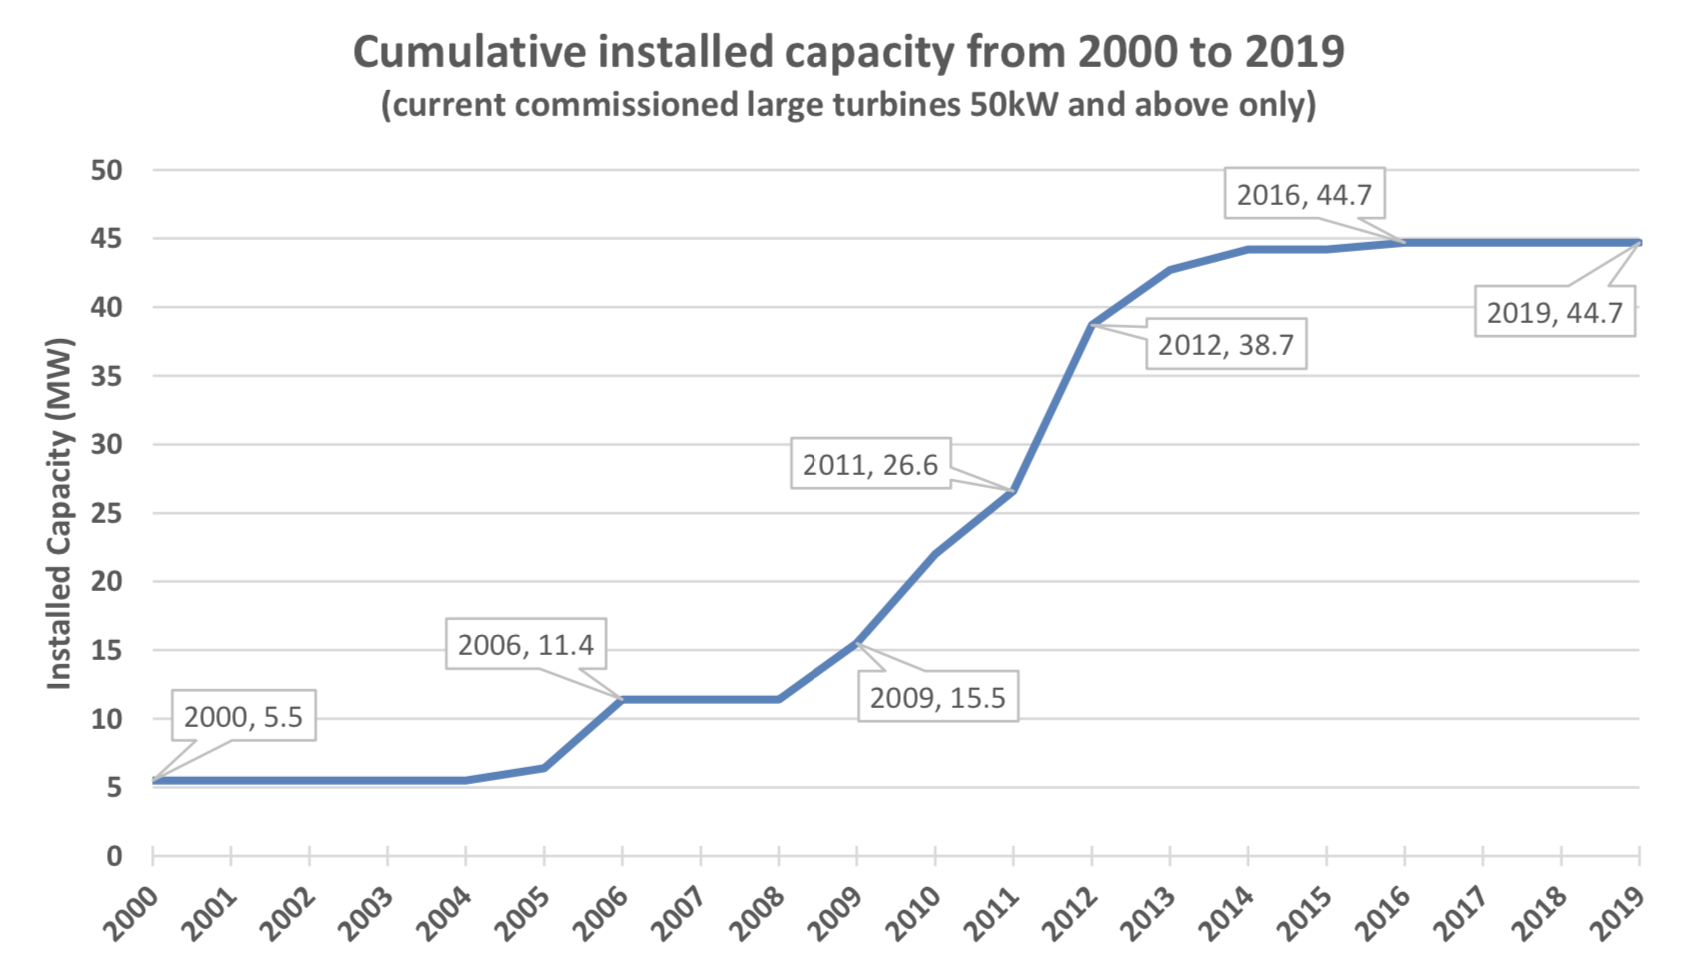
\includegraphics[scale=1]{cummulativewindcapacity}}
            \caption{The cumulative wind power generation capacity between 2000 and 2019}
            \label{fig_cummulative_wind_capacity}
        \end{figure}

        To increase hydropower capacity, a project called \emph{Surf`N'Turf} was launched to build hydrogen storage in Eday, 
        which includes three tube trailers each capable of storing 250kg of hydrogen and one 500kg static hydrogen storage \cite{website:surfturf}. 

        In the past few years, some transitions of electrification have been posed; 
        like increasing the number of electrical vehicles (EVs) and ferries (EFs) to switch 
        from fossil demand to electricity demand, improving the gas heating types of 
        equipment to the electrical heating ones, and installing wind turbines with local 
        storage for households to achieve energy trades among customers. 
        Additionally, the number of EVs has been increasing drastically from a relatively small group to 234 in the first quarter of 2019 \cite{report:OrkneyAudit}, as is indicated in \hyperref[fig_EV_number]{Figure \ref*{fig_EV_number}}.
        The rate of growth is 975\% in 5 years. The reason of this high grow speed is that on the one hand distributed wind turbines and local energy reserve storage can be installed in Orkney, which increase the accessibility of electric power with cheaper price, on the other hand, the community of Orkney provides charging stations which can charge EVs without fee (This service was turned to be paid charging scheme in 2019 April \cite{report:OrkneyAudit}).

        \begin{figure}[ht]
            \centerline{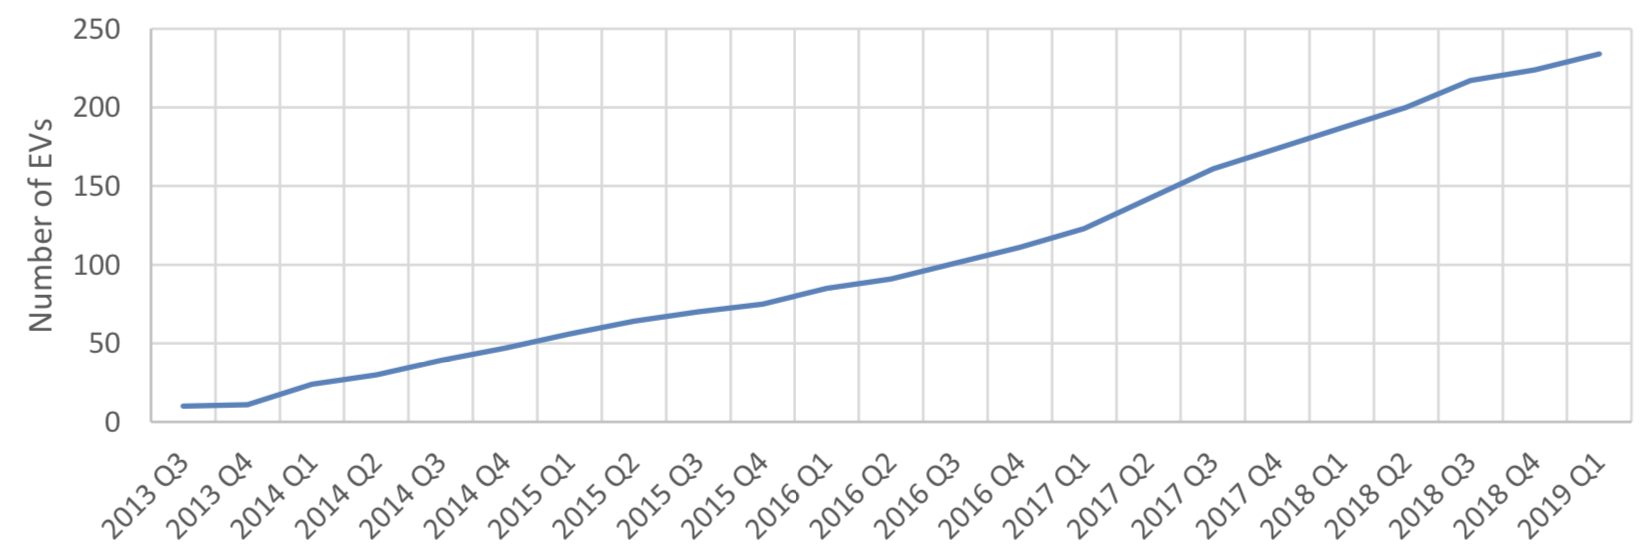
\includegraphics[scale=1]{evnumber}}
            \caption{The EV number evolution from 2013 to 2019}
            \label{fig_EV_number}
        \end{figure}

        To solve this problem, the over generated energy can be exported to the mainland of UK via a 20MW transmission line \cite{book:Orkneypowerexport}. 
        However, there is still 16\% wind power generation having been curtailed in the last year \cite{report:OrkneyAudit}, which implies that the current wind power capacity has been excessive.
        
        Under the analysis of local power demand and generation, it is possible to estimate the amount of local storage in an appropriate range and determine its technique. 
        However, it is estimated that 99\% of the total power generation in Orkney is from the wind \cite{report:OrkneyAudit}, 
        which is intermittent in nature. Its large variance leads to an unstable connection to the grid, 
        which imposes large challenges to the design of the storage.

        The characteristics of typical storage technologies are summarizes in \hyperref[table_storage_characteristics]{Table \ref*{table_storage_characteristics}} \cite{paper:Barton2004} \cite{paper:Vazquez2010}.

        \begin{table}[ht]
            \begin{tabulary}{\linewidth}{c L L L L}
                \hline
                Type & Energy efficiency (\%) & Energy density (Wh/kg) & Life cycle (cycles) & Services \\ \hline
                \hline
                Ni-Cd & 60 - 90 & 40 - 60 & 500 - 2000 & Wind power smoothing, spinning reserve \\ \hline
                Li-Ion & 70 - 85 & 100 - 200 & 500 - 2000 &  Wind power smoothing, spinning reserve, PV, portable devices\\ \hline
                Ni-MH & 50 - 80 & 60 - 80 & $<$ 3000 & Wind power smoothing, spinning reserve, PV, portable devices \\ \hline
                Pumped hydro & 65 - 80 & 0.3 & $>$ 20 years & Daily load cycle, weather variations \\ \hline
                Flywheel & 95 & 5 - 30 & $>$ 20000 &  Wind power smoothing, spinning reserve \\ \hline
                Super-capacitor & 100 & - & - & Voltage and frequency control, governor controlled generation \\ \hline
            \end{tabulary}
            \caption{Storage technologies and characteristics}
            \label{table_storage_characteristics}
        \end{table}

        \section{Establish a data set from available source}
        A data set is constructed to acquire understanding of power generation and demand in Orkney. The data set began to scrape data from 19th October. 
        This section describes the available data source used in this constructing the data set and the details on implementation.

        \subsection{Data sources}
        The data set contains data of three parts: generation and demand in Orkney, curtailment status in Orkney and the weather in Orkney.

            \subsubsection{Generation and demand data source}
            \label{text_generation_and_demand_data_source}
                The ANM website \cite{website:ANM} contains a bar chart to indicate the current power generation and demand of the whole
                island. Figure \ref{fig_anm_barchart} shows this chart. There are 5 records: Live Demand, Winter Peak Demand, Orkney ANM, Non-ANM Renewable Generation, Total renewable capacity.
                Some explanations of them can be found in the left of the web page.
                However, the website itself does not expose APIs to get these data, thus it is necessary to analyze its http request and response and use a 
                server to scrape the data periodically.

                \begin{figure}[ht]
                    \centerline{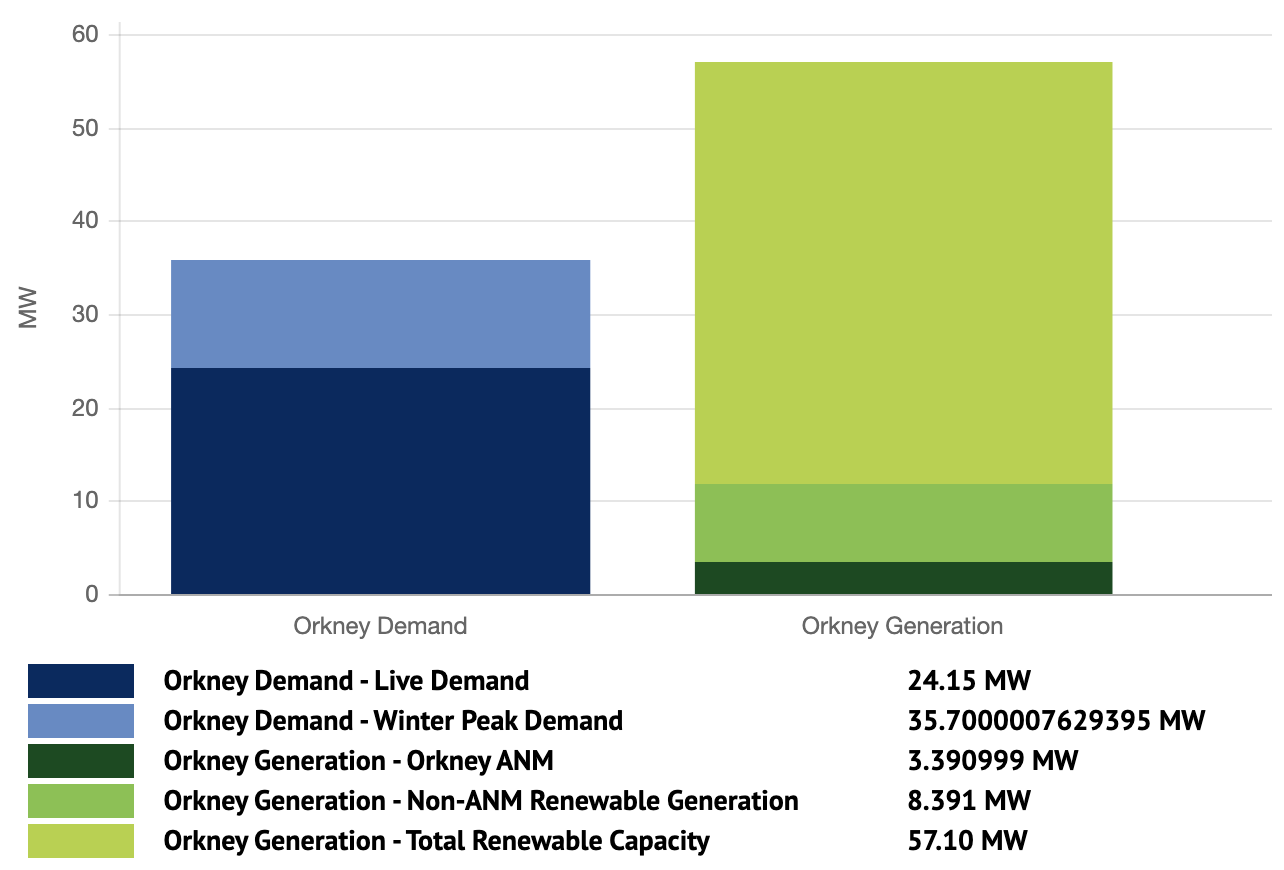
\includegraphics[scale=1]{anm_barchart}}
                    \caption{The Orkney Live bar chart to represent the energy generation and demand of the island}
                    \label{fig_anm_barchart}
                \end{figure}
            
            \subsubsection{Curtailment data source}
                On the ANM status website \cite{website:ANMstatus}, the island is divided into 9 zones as it is indicated in Figure \ref{fig_map}. Then there is a 
                table contains the current status of each zone. Unfortunately, there are neither public APIs to extract these data. The same method should
                be applied to scrape the data from this website.

                \begin{figure}[ht]
                    \centerline{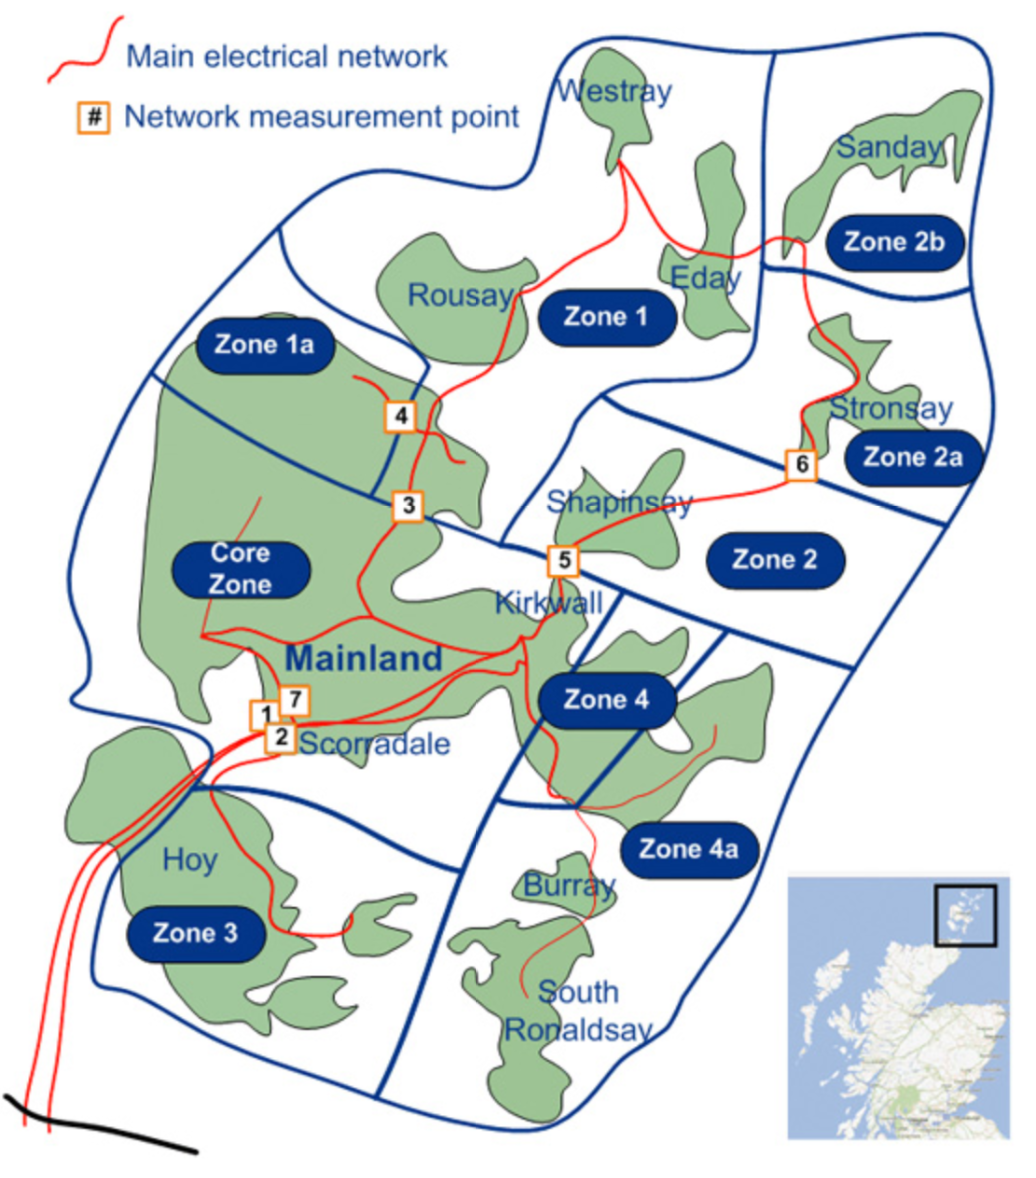
\includegraphics[scale=1]{map}}
                    \caption{ANM zones}
                    \label{fig_map}
                \end{figure}
            
            \subsubsection{Weather data source}
            \label{text_weather_data_source}
                The Open Weather Map website \cite{website:OpenWeatherMap} provides public APIs to clients to get weather information of all over the world.
                Depending on the functions, some APIs which can request for historical data are paid services and the free ones can only acquire data at current time point.
                As the former two sources are both extracted from real time, it is not necessary to get historical data. The free APIs are used to get the weather
                information in Orkney. Various kinds of weather information are available from this API, such as temperature, visibility, wind speed and degree, and clouds.
                As only the wind speed is directly related to wind power generation \cite{paper:Shao2010}, it is selected along with the temperature and humidity to be recorded in the data set.
            
        \subsection{Tools and implementations}
        The data set is established on a cloud server with Cent OS 7 installed. As the data needs to be requested periodically all the time, a cloud server is the most
        efficient method. The scripts used in scrape the data are written in python 3 \cite{website:python3} and bash \cite{website:bash}. Libraries and tools based in these two languages are mentioned below.

                \subsubsection{Fetching Generation and demand data}
                By tracing the http response and request, the from of the generation and demand data are transformed in a JSON format file. Then, it is possible to 
                use the Request python library \cite{website:requestpython} to imitate this http request and receive this file. After parsing the content, current power generation and demand data can
                be extracted and stored in the database built on the server. The store and program launch actions are controlled by crontab \cite{website:crontab} to execute in a 10-minute period.

                \subsubsection{Fetching curtailment data}
                \label{text_fetching_curtailment_data}
                The form of curtailment data is not JSON as it is embedded in the html file fetched from the request. The web page contains some javascript programs which demonstrate information
                on the table. Because this file is a mixture of programming logics and data, it cannot be analyzed using a JSON parser as the generation and demand data did. The method is that, first
                save this html file as a text file to the disk, then use grep \cite{website:grep} to find the clauses which contain the status data. The status data is again saved as a file. Relaunch
                a python script to parse this simplified file and store the data of the table to the local database. The Status of the zone is represented using 1s and 0s, as it is assumed that the state
                of each zone can only be off and on. Actually, there is one more state called partly off which was not noticed when writing the script file, thus only two states are recorded.

                \subsubsection{Fetching weather data}
                As the APIs are provided, the implementation is that to write a python script using a library which wrap the API functions of Open Weather Map in python \cite{website:pyowm}.
                Use the verification code provided after registering a client of the website and find the region code of Orkney, then the weather condition can be fetched in JSON format. Apply
                the same procedure are the power generation and demand data to store the weather data in the database.

                \subsubsection{Synchronizing database to local} 
                The database in the cloud server needs to be synchronized periodically to avoid possible loss due to abrupt. The method is to use github \cite{website:github}. Create a git repository \cite{website:git}
                and add the database file into it. Then, use crontab to execute a push command of git to synchronize the repository on the remote server of github. To access the repository on remote server, it is mandatory
                to enter login id and password of a github user. As it is using crontab to synchronize, the interaction of git push will cause problems. The solution is to use the pexpect library \cite{website:pexpect}, which
                create a shell for each command needs interaction and interact with that command as the user defined. After solving this problem, the database can be updated without manually controlling extra steps. When it is
                needed for the user to get or update the data set, directly pull the repository from github, as it is always synchronized to the cloud server. The frequency of synchronization is set at 12:30 every day.

                \subsubsection{Data analyzing and visualizing}
                Various libraries are used. The Numpy and Scipy libraries \cite{website:numpy} \cite{website:scipy} are used to process statistical and vector-based computing. The Pandas library \cite{website:pandas} is used
                to loading data set into memory and applying complex data set enquiries. The Scikit-Learn library \cite{website:scikit} provides machine learning models and data preprocessing methods. The matplotlib library
                \cite{website:matplotlib} provides plotting and rendering tools to produce plot. These libraries all provide APIs in python. Thus, python programming language \cite{website:python3} is used. Another reason is that
                the task of data analyzing is generally classified to fast development, as the cycle of editing code and fetching the results must be short. The programming language python \cite{website:python3}, which is a
                dynamically typed and script-based language, is satisfying all demands. Further more, the browser based programmable Jupyter notebook under Jupyter Project \cite{website:jupyter} provides a flexible and user-friendly
                UI for programming using python. This makes visualizing data like plots and tables in an easier and more efficient way.
                
        \subsection{Data bias and loss}
        It is definite that the data accuracy is limited under various reasons. No data sources listed above has the guarantees or warranties that the data is accurate, complete and up-to-date. 
        Since they are the only sources for Orkney, there are not other choices.

                \subsubsection{Sample loss}
                As it has been mentioned above, the sample rate is 10 minute. That is to say information between two neighboring sampling slots is out of observation.
                If some fierce disturbances happen at that interval, this information is lost because of low sampling rate. However, the ANM website does not provide
                the definition of the real-time data, nor data of each zones. Additionally, the data of the over-all island has been in aggregation pattern that cannot
                indicate spikes caused by individual household load or power generation. It is assumed that the information in each 10-minute interval is recoverable be
                observing its two neighboring samples.

                \subsubsection{Source stability}
                \label{text_source_stability}
                Under the assumed sample rate, there should be $6*24=144$ samples of each attribute each day. However, there are not always 144 samples in a one-day period.
                For example, the number of samples of the whole November should be $24*6*30=4320$, but the data set only contains $4252$ samples. There are $68$ 10-minute samples
                lost. Additionally, from iterating these samples day by day, there are only two days satisfying the assumption of $144$ samples a day. Most of the days contain
                $141$ or $142$ samples. The reason is that the ANM website always runs into corruption: the website cannot response to the requests and accessing through browser results
                in another page of maintenance. It seems that it will become blocked for a very short period each day from the samples. However, it is recorded that the website
                went to a longer corruption from 13th December to 19th December and 25th January to 29th January.

                The methods of analyzing data of time series in this project are all designed under the presumption that there are no samples lost. The days without enough samples cannot be
                used sequentially. However, if only several days with enough samples are used, there will be only two days in November. There are just one or two samples missing for most of the days.
                Thus, it is possible to recover these lost samples from linear prediction of samples before and after the point. A method of fix these loss points is discussed
                in Data cleaning section. Under the condition that the sample of half or the whole day is lost, there is not possible ways to recover, thus, these days are excluded from
                analysis.
            
                
        
        \section{Statistical analysis}
        To analyze energy scenarios in Orkney, some statistical tools have been used in this project.
        This section summaries concepts and tools used in statistical analysis.
        
        \subsection{\emph{Covariance} and \emph{Correlation}}
        % It is necessary to find the relationship of two attributes in data analysis. For example, the wind speed and the wind power generation, the power demand on timeseries of two days. The properties discussed above can only be used to analyze single variable. To find information about the relation of two variables or their tendency to vary together, the concepts of \emph{covariance} and \emph{correlation} are introduced.

        The \emph{covariance} of two random variables $X$ and $Y$ is define as:
        \begin{equation}
            Cov(X,Y)=E[(X-E(X))(Y-E(Y))]
        \end{equation}

        It gives a measurement of the degree of $X$ and $Y$ vary together. However, this numeric value is influenced by the magnitudes of $X$ and $Y$. For example, $Cov(2X,Y) = 2Cov(X,Y)$. Thus, the definition of \emph{Correlation} is introduced:
        \begin{equation}
            \rho(X,Y) = \frac{Cov(X,Y)}{\sigma_X \sigma_Y}
        \end{equation}

        It can be verified that $ -1 \leq \rho(X,Y) \leq 1 $ \footnote{\emph{Cauchy-Schwarz Inequality}}. It is said that $X$ and $Y$ are \emph{positively correlated} is $\rho(X,Y) > 0$, that $X$ and $Y$ are \emph{negatively correlated} if $\rho(X,Y) < 0$, and $X$ and $Y$ are \emph{uncorrelated} if $\rho(X,Y) = 0$.

        \subsubsection{\emph{Correlation Matrix}}
        In pragmatic analysis, the \emph{Correlation Matrix} is a common method to measure the relationships among at least 2 attributes. Assume the number of attributes is $N$, the \emph{Correlation Matrix} is calculation the \emph{Correlation} between each pair of attributes. The \emph{Correlation} between the $ith$ and $jth$ attributes, $corr(attr[i],attr[j])$, is located in the $a_{ij}$ and $a_{ji} $ entries. For example, \hyperref[table_correlation_matrix_monday_demand]{Table \ref*{table_correlation_matrix_monday_demand}} calculates the \emph{Correlation Matrix} of the demand of Mondays to find their degree of variations. It can be figured out that the diagonal entries are always 1 as it is the \emph{Correlation} is itself.
        
        
        \subsection{Regression models}
        The Regression method is used to quantize the relationship among attributes as the \emph{Correlation matrix} merely provides the degree of relation. Parameters are derived from regression models in order to infer from known attributes to the attributes with strong relation. For example, the wind speed is related to the wind power generation and a regression model constructed to predict the wind power generation from the wind speed is shown in \hyperref[text_wind_regression_model]{Section \ref*{text_wind_regression_model}}.
        The fundamental concepts are introduced in this section.

        \subsubsection{Linear Regression model}
        The linear regression model can be characterized with a set of parameters: $\Theta$, which quantize the relation between the target $y$, and the attributes $x$:
        \begin{equation}
            y = \theta_0 + \theta_1 x_1 + \theta_2 x_2 + \,...\,+\theta_nx_n
        \end{equation}
        In this formula, the target $y$ can be seen as a weight sum of attributes $x$ plus a bias $\theta_0$. 
        
        % If these parameters are carefully selected and trained by regression methods, there is enough confidence to predict $\hat{y}$ which is near the actual value $y$ within an acceptable error tolerance.
        % \begin{equation}
        %     \hat{y} = h_\theta(x) = \bf{\theta}\, \cdot \,x
        % \end{equation}

        % To determine the values of $\theta$, the basic solution is to extract $\hat{theta}$ from the matrix multiplication:
        % \begin{equation}
        %     Y = X\, \bf{\hat{\theta}}
        % \end{equation}
        % where the dimension of $Y$ is $ n*1$, and that of $X$ is $n*m$, with $n$ as the number records of $x$ to $y$, and $m$ as the number of attributes.
        % To isolate $\bf{\hat{\theta}}$, it is easy to merely multiplicate $X^{-1}$ to the left. However, this operation implicitly assumes $X$ is a square matrix. Generally, $n \gg m$, as there should be enough samples to calculate a the $\bf{\theta}$ which is universally applicative.

        % As only a square matrix can have the inverse, $X^T$ is first multiplicated to transform the dimension from $n*m$ to $m*m$. Then, the inverse can be calculated as: $(X^TX)^{-1}$, and the parameters can be derived from:
        % \begin{equation}
        %     \hat{\theta} = (X^TX)^{-1}X^TY
        % \end{equation}

        % Actually, modern linear regression models, such as the implementations in Scikit-Learn \cite{website:scikit}, do not use this formula. There are two reasons. One is that it cannot be guaranteed that $X^TX$ is not singular, which leads to trivial solutions. The other is that the complexity of this formula is $O(n^3)$, which makes the computation slow with large $n$ \footnote{Assume the size of $n$ is 10 times than before, then it results in the time of computing $\hat{\theta}$ 1000 times larger than before.}.

        % The method is to use the \emph{Pseudoinverse matrix} of $X$: $X^+$, which is computed useing \emph{Singular Value Decomposition (SVD)}. This matrix can be computed even $X^TX$ is not invertible, and the complexity is $O(n^2)$. The details of this theory can be found in Gilbert Strang \cite{book:linearalgebra}, and one of its implementation can be found in numpy.linalg.svd() \cite{website:numsvd}.

        \subsubsection{Gradient Descent}
        % Apart from the methods based on matrix, another algorithm has also been widely used as optimization. 
        \emph{Gradient Descent} uses the slop of the cost function to find the parameters of the model. By calculating derivation on the cost function \footnote{Normally, the \emph{Mean Squared Error (MSE)} is used: $$MSE(\theta)=\sum_{i=1}^m\frac{1}{m}(\theta^T x^{(i)} - y^{(i)})^2$$ which is also known as the \emph{norm-2} metric emphasizing the \emph{mean} of distribution of the error.}, the slops of each parameter tell the direction it grows fast. Thus, the negative of the slops can be chosen and added to the parameters to form a set of new parameters. Each projection of $x$ to $y$ can be used to compute a set of new parameters, then this operation can iteratively evaluate the whole set to reach the global minimum of the cost function.

        % Fortunately, the \emph{MSE} is a \emph{convex function} \footnote{The line segment of any two points on the graph of a convex function is above or on the function lines \cite{website:wikiconvexfunction}. It can be expressed as: $$f^{\prime \prime} (x) \geq 0$$}, that is to say, the global minimum can be definitely reached and the optimized parameters can be found. This property is really important for the \emph{Gradient Descent} method, as it may otherwise reach a local minimum, if the function is not convex.

        % Generally, a GD model has two important parameters: \emph{learning rate} and \emph{tolerance}. The learning rate can not be too small or too large \footnote{Too small will lead to reaching the minimum slowly and may take more times on reaching it with a large amount of iterations. Too large makes it hard to stop at the minimum, instead, it oscillates around the minimum.}, and the tolerance applies an acceptable interval to let the calculation stop near the minimum.
        
        % The derivation of \emph{MSE} is:
        % \begin{equation}
        %     \frac{\partial }{\partial \theta_j} \bf{MSE(\bf\theta)} = \sum_{i=1}^m\frac{2}{m}(\theta^T x^{(i)} - y^{(i)})x^{(i)}_j
        % \end{equation}
        % It can be written in vector form as:
        % \begin{equation}
        %     {\nabla}_\theta\bf{MSE(\theta)} = \frac{2}{m}X^T(X\theta - y)
        % \end{equation}

        % Without the calculation on the inverse or SVD \cite{book:linearalgebra} \cite{website:numsvd}, only the product of the matrix is need to be calculated, thus this algorirhm is efficient.
        % But it also has efficacy that the model needs to calculate the whole set during each iteration to make the next step to the minimum, thus it can be slow when the training set is really large. The improved version uses randomly chosen instances to calculate the derivation vector each time. The method is called \emph{Stochastic Gradient Descent (SGD)}. As it only needs to calculate one instance on each iteration, it is efficient on large training set 
        % \footnote{Assume that the training set is $m*n$, then it will be $2mn$ products and $2mn$ sum and $n$ subtracts per iteration for \emph{GD}, compared with that for \emph{SGD}, it is $2n$ products, $2n$ sums and $n$ subtracts. It is obvious that the normal \emph{GD} takes m times time of \emph{SGD} per iteration. When $m$ is large with a generally 1M size, the cost can be significant.} Though, \emph{SGD} needs more iterations to reach the minimum, it is worth the trade-off.

        % Another important improvement on \emph{SGD} is the \emph{Simulated Annealing} learning schedule, which lets the model uses large \emph{learning rate} at the begining, then as the model learns to fit the data set, the rate decays to be more and more smaller to let the model carefully reach the minimum point \footnote{This is a strategy inspired from the process in metallurgy of annealing.}. 

        % \begin{figure}[ht]
        %     \centerline{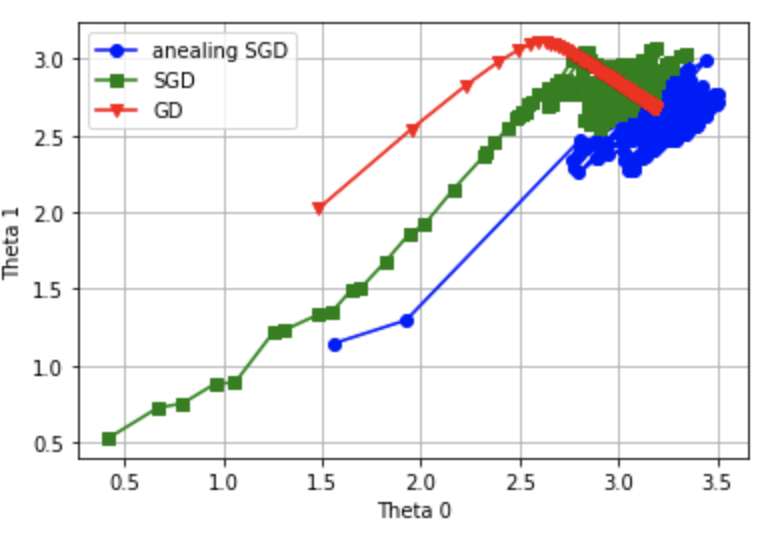
\includegraphics[scale=1.4]{sgd}}
        %     \caption{Visualzation of \emph{GD}, \emph{SGD}, and \emph{Simulated Anealing} characteristics}
        %     \label{fig_sgd}
        % \end{figure}

        % \hyperref[fig_sgd]{Figure \ref*{fig_sgd}} depicts the regression procedure of the three learning methods tested on a model with one attributes \footnote{As it has been discussed, $\theta_0$ is the bias.}. It can be seen that the basic \emph{GD} method becomes unefficient when it reaches near the minimum \footnote{The speed becomes much slower that before after the direction of $\theta_1$ changed at about 3.2.}. The \emph{SGD} has an undeterministic speed and it oscillates near the minimum. The \emph{Simulated Anealing} has a large speed at the beginning, and the speed is decayed as the iteration grows.

        \subsubsection{Polynomial linear regression model}
        When the linear regression can not have better fitness with the power of 1 for the attributes, the polynomial linear regression is introduced, with can extend the power of each feature to n.

        For example, for a vector $x = [a, b, c]$, if it is extended to degree $d = 2$, $x = [a, a^2, b, b^2, c, c^2, ab, ac, bc]$. The number of the attributes (n) will be extended to:
        \begin{equation}
            n_{poly}=\frac{(d+n)!}{d!\;n!}
        \end{equation}

        When the degree of the polynomial linear regression is increased, the cost function is becoming smaller, as the new degree applies more limitation on the model to well fit in the training set.

        There is also a trade-off between the degree and generalization of the model. As high degrees are easy to introduce over-fitting, but that does not mean low degree is good. When the cost function can not decrease to an acceptable range no matter how much data has been fed, it is time to increase the degree. Low degree always introduces under-fitting or high cost function.

        \subsection{Binomial regression}
        The Binomial regression model uses boolean value as the target value. It is used to implement classifier, for example, to judge whether a mail is a junk mail from the information of title, and to identify whether a curtailment has happened based on the wind generation power and demand in this project.
        Because the target attribute is not a numeric value, it is not appropriate to use metrics like \emph{MSE} or \emph{RMSE} to train and evaluate the model. Instead, the \emph{Type I} and \emph{Type II} errors are introduced.

        \subsubsection{\emph{Type I} and \emph{Type II} error}
        \emph{Type I} error is also called false positive, which refers to true hypothesis that is rejected by the decision. \emph{Type II} error is called false negative, which refers to false hypothesis not rejected by the decision. The concepts of these errors can be demonstrated in \hyperref[table_error_types]{Table \ref*{table_error_types}} \cite{website:typeItypeIIerror}.
        \begin{table}[ht]
            \centering
            \begin{tabulary}{\linewidth}{|C |C| C|}
                \hline
                 & True & False \\
                \hline
                Don't reject & Correct inference (true positive) $possibility = 1-\alpha$ & Type II error (false positive) $possibility = \beta$ \\
                \hline
                Reject & Type I error (true negative) $possibility = \alpha$ & Correct inference (false negative) $possibility = 1-\beta$ \\
                \hline
            \end{tabulary}
            \caption{Table of error types}
            \label{table_error_types}
        \end{table}
        
        It is necessary to notice that to eliminate one type error, the other type error must grow, but by selecting a low threshold, an optimal $\alpha$ can be achieved to increase the quality of judgement.

        In the machine learning field, the \emph{Confusion matrix} is implemented based on the error types. It has two rows and two columns which count the predictions under different error types or correct inferences.
        \section{Simulation frameworks}
        To simulate the power grid with high EV penetration and dependence on wind power generation,
        two kinds of simulation frameworks have been considered in this project: \emph{event-driven simulation} and \emph{analytic simulation}.
        Both of them are introduced in this section.

        \subsection{\emph{Event-driven simulation}}
        This simulation framework is mostly used in circuit simulation software design. The basic idea is that the actions will trigger further events happen at a later time. Such events then also act as one action which can cause new events happen at a later time.
        This is a recursive procedure, which starts from an action and ends with all actions processed.

        To elaborate, think of an example from Harold \cite{book:sicp}. 

        \begin{figure}[ht]
            \centerline{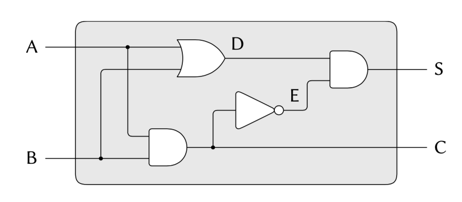
\includegraphics[scale=2.2]{halfadder}}
            \caption{An implementation of Half-adder}
            \label{figure_half_adder}
        \end{figure}

        \hyperref[figure_half_adder]{Figure \ref*{figure_half_adder}} shows a circuit of half adder linked using logical gates. Ports $A$ and $B$ are inputs representing two logical number to be added, $S$ is the sum, and $C$ is the carry. Its bool expression can be written as $S = (A|B)\&\overline{(A\&B)}, C = A\&B$. From both the expression, either a change of $A$ or $B$ will result in the changes on $S$ and $C$.
        Assume $A = 0$ and $B=0$, causing $S = 0$ and $C = 0$. At time $t=0$, $A$ is changed from $0$ to $1$. As $A$ is linked to \emph{OR-gate} D and \emph{AND-gate} F, this will drive the output of D to $1$ at a later time (an interval of \emph{OR-gate delay}). After the delay, the output of D changes to 1, this change becomes an action to the \emph{AND-gate} of $S$ and triggers a change after a \emph{AND-gate delay}.
        The wire $S$ has a new value after the delay, and the simulation system stops as there is no new action triggered by $S$.

        The key to this simulation scheme is a structure called \emph{Schema} \footnote{One implementation is a record of an integer value which represents the current time and a table of which the tuple is a record of an integer value which represents the specified time and a list of actions which are procedures on the wires. The wire can also be a record of a value and a list. The value is its current state: $0$ or $1$. The list is the actions added by each logical gates. So that when the value is changed by a start action or other triggered events, the actions are performed to propagate the effects and trigger further events to the gates `after it'.}, which stores the information of the current time, and the \emph{agenda} which stores the actions that should be processed at a specified time. The simulation processing logic is to compare the current time and the specified time of the first \emph{agenda item} in the \emph{Schema}. If the two values are equal, process the actions in that \emph{agenda item}. If they are not equal, update the current time by an increase. After processing the the actions in one \emph{agenda item}, new actions may be added to be processed at a later time, and the current \emph{agenda item} is deleted. After the deletion, the originally second \emph{agenda item} becomes the first the \emph{agenda item} and the procedure calls itself at the end to perform a tail iteration. The procedure then run to the next \emph{agenda item} with the same logic till there are no \emph{agenda items} in the \emph{agenda table} which denotes the end of the simulation.

        Apart from the trigger propagation strategy, a log system is a necessary part of simulation framework, as it is the interface to the users to check simulation details and results. There are two available strategies: time-based log and event-based log. The differences can be understood from literal meaning that the time-based log records the state of each component on every time slot \footnote{Every time the current time in the \emph{Schema} is updated, the logger will record the states of all components. Thus, the time-based logger structure is a timetable.} and the event-based log records the information of a state change of one component \footnote{It can be embedded with the \emph{Event-driven} strategy as an action of the wire as a possible implementation. The structure is thus a diary.}. Generally, it is reluctantly to tell which is better, as the log can be converted or interpreted to the opposite form. It is the complexity of adding it to the specific simulation framework that causes the priority. For example, the lionized idea of the discussed digital circuit simulation system is based on \emph{Event-driven} strategy. A event-based logger system can be implemented by adding a new action called \emph{probe} which writes information of a state change to a log file whenever it is called. This new action is added to any wire to be logged and the details of log item can be changed by merely editing this action. However, if using the time-based log, the logger cannot be implemented as an action as the action is only called when it is triggered. It should be new structure which records each wire in the circuit. When the current time is updated in the \emph{Schema}, the logger procedure is launched to read this structure and record the state of each wire. Obviously, there are cumbersome codes to write for this logger.

        \begin{figure}[ht]
            \centering
            \begin{tikzpicture}[
                roundnode/.style={circle, draw=gray!80, fill=gray!15, very thick, minimum size=7mm},
                rectanglenode/.style={rectangle, rounded corners, draw=black, fill=gray!20, very thin, minimum size=5mm},
                rectanglenode2/.style={rectangle, rounded corners, draw=black, fill=white, very thin, minimum size=5mm},
                arrow/.style={thick,->,>=stealth}
                ]
                \node[rectanglenode, text width = 2.8cm] (firstnode) {\emph{main simulation process logic}};
                \node[rectanglenode] (secondnode) [below=0.6cm of firstnode.south] {Model components};
                \node[rectanglenode, inner xsep = 2.5cm, inner ysep = 0.7cm] (schema) [right=1cm of firstnode.east] {};
                \node at (schema.center) [above] {\emph{Schema}};
                \node[rectanglenode2] (currentTime)at (schema.base) [below left] {Current time};
                \node[rectanglenode2] (agenda) at (currentTime.east) [right=0.47cm] {\emph{agenda}};
                \node[rectanglenode, inner xsep = 2cm] (logger) [below=0.4cm of schema.south] {logger};
                \draw[arrow] (firstnode) -- (secondnode);
                \draw[arrow] (firstnode) -- (schema);
                \draw[arrow] (logger) -- (secondnode);
                \draw[arrow] (secondnode) -- (schema);
            \end{tikzpicture}
            \caption{Structure of \emph{Event-driven} simulation framework}
            \label{fig_structure_of_event_driven}
        \end{figure}

        \hyperref[fig_structure_of_event_driven]{Figure \ref*{fig_structure_of_event_driven}} shows the basic structure of a \emph{Event-driven} simulation system. Fow a power grid simulation system, the model components could be wind power generator, grid, EV, house, appliance. The state should be the time, because the consumption is assumed to be a function of time, for example, the household demand profile in \cite{report:household} is a function of time of the day, the season, the house type and house owner.

        \subsection{\emph{Analytic simulation}}
        \label{text_nasa_trick}
        Unlike the former strategy, this strategy is more generally applied, as its idea is easy to understand: analyze the model based on a some variables \footnote{Usually take the time as the variable, as most real-world model are based on time, or should be simulated by time.} for a specified amount of cycles. The core of this framework is the \emph{scheduler}, which initialize the model, run analytic functions for instructed number of cycles and terminate the model. It is like the \emph{Schema} in previous framework, but all of the actions have been determined before the simulation begin, and no new actions will be added during simulation. The action in the \emph{Analytic simulation} is called the \emph{Scheduled job} which is provided by the model.
        Take the power grid as an example. Models of grid, wind generation, house, EV and other objects in one grid should be implemented first, so that they can be added to the scheduler to be initialized. These models should contain an analytic function to be called on each simulation cycle by the scheduler, a termination function to be called at the end of the simulation, to summarize the results, such as the average value, the score of special metrics.

        In this project, a simulation environment based on \emph{Analytic Simulation} called \emph{trick} \cite{website:trick} is used for simplicity. The reason is that it provides the interface of implementing model in \emph{C/C++}. Then the jobs can be scheduled using a script which includes the model and functions exposed to be called for initialization, analysis, and termination. Additionally, a versatile logger is provided, for example, it can automatically parse the source code of model and extract possible variables to be recorded. Because of this, the documentation also elaborates a special style of comment which can be understood by the interpreter to make sure the properties are rightly unified \footnote{Because of this function, the data recording function can convert all the variables automatically to the same unit. This release possible work of converting from users.}, such as the unit, i/o, and type. This framework also provides \emph{Monte Carlo} simulation method, which can repeatably run copies of a simulation with different input values. By calculating values from previous \emph{Monte Carlo} runs, optimization can be achieved.
        For the design of \emph{Monte Carlo} simulation, \hyperref[fig_master_controller]{Figure \ref*{fig_master_controller}} depicts the master controller, and \hyperref[fig_slave_controller]{Figure \ref*{fig_slave_controller}} shows the slave controller.

        \begin{figure}[ht]
            \centerline{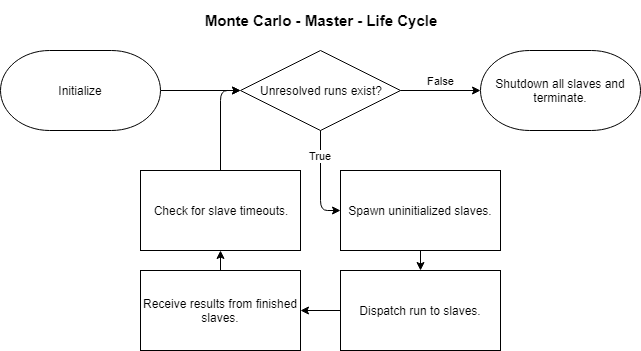
\includegraphics[scale=0.6]{MonteCarlo-Master-LifeCycle}}
            \caption{Master controller of \emph{Monte Carlo} simulation in \emph{Trick}}
            \label{fig_master_controller}
        \end{figure}
        The master controller for any given Monte Carlo simulation delegates run information to distributed slave instances. The master is responsible for spawning and managing the state of all slaves for a given simulation.

        \begin{figure}[ht]
            \centerline{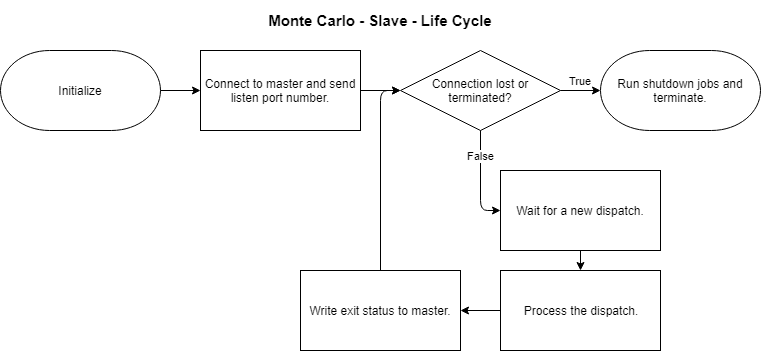
\includegraphics[scale=0.5]{MonteCarlo-Slave-LifeCycle}}
            \caption{Slave controller of \emph{Monte Carlo} simulation in \emph{Trick}}
            \label{fig_slave_controller}
        \end{figure}
        A Monte Carlo slave simulation is responsible for the execution of the runs delegated by the master controller. Should a simulation run fail, the slave will inform the master and continue running until explicitly killed or disconnected. Slaves consume only a single CPU and run only one job at a time. If you want to increases parallelism, you should create multiple slaves. Creating one slave per CPU is a reasonable approach.
        \section{Household loading profile}
        \label{text_household_loading_profile}
        In \hyperref[text_simulatinghouseholdload]{Section \ref*{text_simulatinghouseholdload}}, a daily household loading profile is needed to support simulation. The basic strategy is to first divide all electrical devices to three types based on their behaviors, and apply each appliance with the model of its type and general consumption data. A research has been delivered in \cite{paper:devicestypes}, and the results can be summarized in \hyperref[table_electrical_devices]{Table \ref*{table_electrical_devices}}.

        \begin{table}[ht]
            \centering
            \begin{tabulary}{\linewidth}{|p{1.1cm}|p{3.3cm} | p{3.3cm}| p{3.3cm}|}
                \hline
                 & Even-smooth type & Stochastic behavior type & Fixed-program type \\ \hline
                 Device & Fridge freezer, Wine cabinet & TV-set, Total light, Electrical cooker, Microwave, Dish washer, Washing machine, Clothes dryer & Water heater, Air conditioner \\ \hline
                 Feature & Base load, Continuously working, Smooth load, Low power consumption & Randomly plug in, Randomly working period, Possible peak load, Medium power consumption & Randomly plug in, Fixed working period, High power consumption \\
                \hline
            \end{tabulary}
            \caption{Typical household electrical devices}
            \label{table_electrical_devices}
        \end{table}

        To model the Even-smooth type device, the consumption is generated periodically. To model the Stochastic behavior type and Fixed-program type, statistical algorithms are used to simulate the randomness. Typical consumption data is extracted from the UK household electricity survey \cite{report:household}.

        \section{EV charging profile}
        \label{text_EV_charging_profile}
        Three categories of typical voltage and power levels of EV charging have been derived from \cite{paper:evchargingprofile} and summarized in \hyperref[table_standard_electric_vehicle_charging_level]{Table \ref*{table_standard_electric_vehicle_charging_level}}.
        The Level 1 and Level 2 are mostly used in single-family residential and multifamily residential. Level 3 is for commercial situations. These three charging consumptions are defined by the Society of Automotive Engineers \cite{website:sae}, and all U.S. EV makers must follow this standard.
        \begin{table}[ht]
            \centering
            \begin{tabulary}{\linewidth}{|C | C | C | C | C|}
                \hline
                 & Voltage (VAC) & Current (Amps) & Power (kVA) & Phase \\
                \hline
                Level 1 & 120 & 12 & 1.44 & Single \\ \hline
                Level 2 & 208/240 & 32 & 6.7/7.7 & Single \\ \hline
                Level 3 & 208/480/600 & 100 & 16.8 & Three \\
                \hline
            \end{tabulary}
            \caption{Standard Electric Vehicle Charging Level}
            \label{table_standard_electric_vehicle_charging_level}
        \end{table}

        In addition, \hyperref[table_typical_ev_charging_time]{Table \ref*{table_typical_ev_charging_time}} provides typical charging time for various sizes of EVs.

        \begin{table}[ht]
            \centering
            \begin{tabulary}{\linewidth}{|C | C | C | C | C |}
                \hline
                EV Configuration & Battery Size (kWh) & 120 V and 12 Amps & 240 V and 32 Amps & 480 V and 100 Amps \\
                \hline
                PHEV-10 & 4 & 3h 5m & 35m & n/a \\ \hline
                PHEV-20 & 8 & 6h 10m & 1h 10m & n/a \\ \hline
                PHEV-40 & 16 & 12h 20m & 2h 20m & 63m \\ \hline
                BEV & 24 & 18h 30m & 3h 30m & 1h 34m \\ \hline
                PHEV Bus & 50 & n/a & 5h 50m & 3h 17m \\
                \hline
            \end{tabulary}
            \caption{Typical EV Charging Time}
            \label{table_typical_ev_charging_time}
        \end{table}

        Combine the information of two tables, the Level 1 charging is more suitable for charging overnight, and Level 2 could be the standard method of charging as it support all five types. Level 3 is designed for public charging facilities for large types of EVs.

        However, these profiles only estimate ideal conditions where the charging outlets are fully powered and the EVs have run out of battery capacity. 
        
        
        \begin{figure}[htbp]
            \centerline{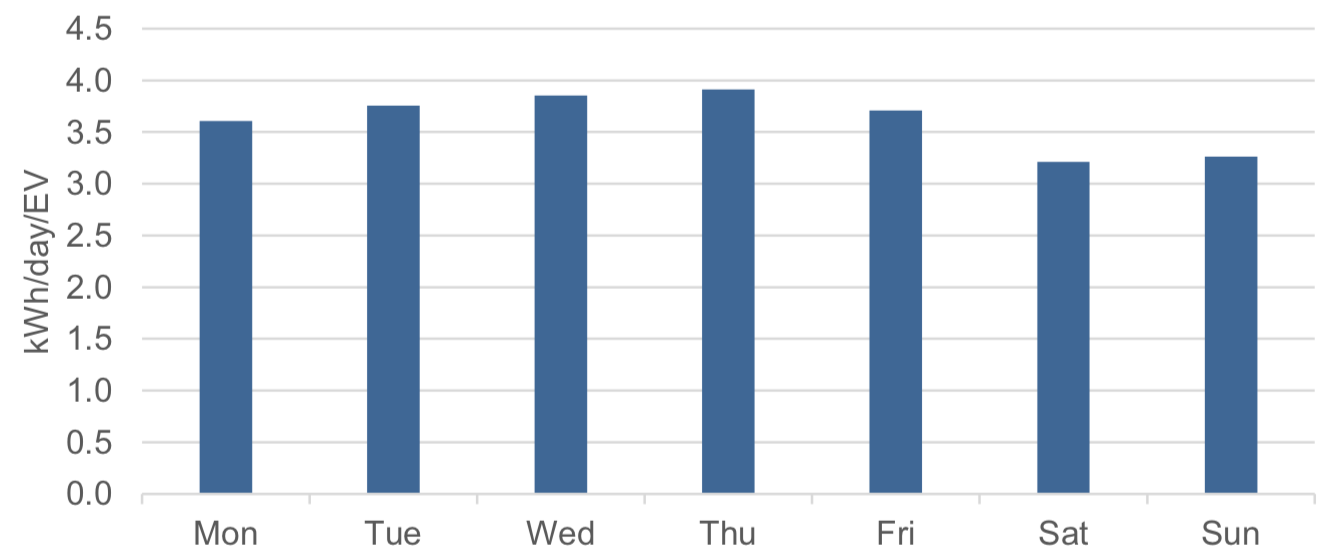
\includegraphics[scale=1]{averageEVchargingamount}}
            \caption{Average kWh/day over course of week for residential charging for an average EV}
            \label{fig_average_ev_charging}
        \end{figure}

        In the Electric Vehicle charging behavior study \cite{report:EVchargingstudy}, the amount of demand of an average EV and the time of charging differs from different week days as it is demonstrated in \hyperref[fig_average_ev_charging]{Figure \ref*{fig_average_ev_charging}}.

        The amount is merely reaching 4.0 kWh for an EV, thus it should be acknowledged that if the EVs are recharging every day, they are not likely to cost as much as the time in the table. A daily trend can also be detected that there is a gradual increase between Monday to Thursday before a slight decrease on Friday and then a lower level on Saturday and Sunday.
        The distribution of charging demand among the period of a day is also studied in \hyperref[fig_weekly_demand_profile]{Figure \ref*{fig_weekly_demand_profile}}. The profile indicates a demand peak on evening time with a maximum between 7-8pm on weekdays and 6-7pm on weekends. The demand profile spread broadly on weekends with a lower maximum.

        \begin{figure}[htbp]
            \centerline{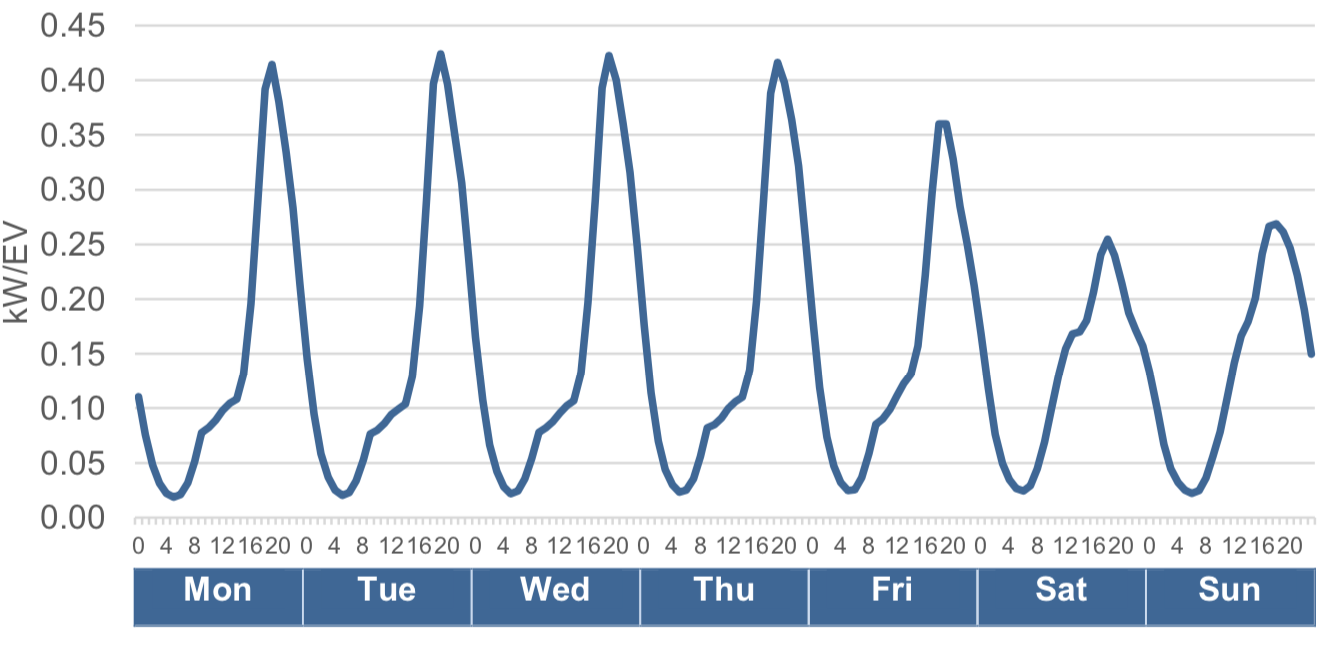
\includegraphics[scale=1]{EVchargingdistribution}}
            \caption{Weekly demand profile of an average EV for residential charging}
            \label{fig_weekly_demand_profile}
        \end{figure}

        Additionally, this demand profile can be combined with the histogram of departure and arrival of a typical household in \hyperref[fig_arrival_vs_departure]{Figure \ref*{fig_arrival_vs_departure}}. The departure behaviors can be projected to the low demand in the morning, and the arrivals in the evening indicates that people are recharging their EVs, thus this results in a peak demand in that morning.

        \begin{figure}[htbp]
            \centerline{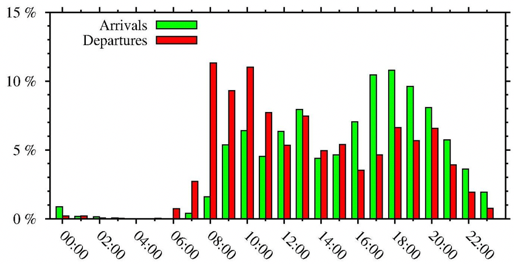
\includegraphics[scale=1.9]{evdepartures}}
            \caption{Arrival and departure study of a day}
            \label{fig_arrival_vs_departure}
        \end{figure}

        The statistics of EVs in Orkney is summarized in \hyperref[table_current_condition_of_EVs]{Table \ref*{table_current_condition_of_EVs}}, which is derived from \cite{report:OrkneyAudit}. The number of EVs in Orkney takes up to 1.4\% of all vehicles on the island. This number is much lower than the predicted penetration of 35\% in 2020 from \cite{paper:PieltainFernandez2011}. It is expected that the number will grow dramatically in the following years, as the electrification of the island has brought large opportunity and merit to transform to EVs. Later, analysis on current EV penetration and higher penetration levels will be performed, and the impacts can be quite obvious under large penetration levels.

        \begin{table}[htbp]
            \centering
            \begin{tabulary}{\linewidth}{|C | C | C | C |}
                \hline
                Average Miles Per Day & Average MWh Per Mile & Number of EVs Registered in Orkney & Estimated Annual Energy COnsumed by Orkney EVs (MWh) \\ \hline
                21.74 & 0.000299 & 234 & 555 \\
                \hline
            \end{tabulary}
            \caption{Current condition of EVs in Orkney}
            \label{table_current_condition_of_EVs}
        \end{table}

        % \section{Methods on exploring impacts of different levels of EV penetration in grid}
        % The instant power consumption of the charging outlets shown in \hyperref[table_standard_electric_vehicle_charging_level]{Table \ref*{table_standard_electric_vehicle_charging_level}} implies that a lot of EVs charging at the same time will increase the peak demand and may cause the instability of the grid. Previously, many papers have focused on this scenario.

        % Three levels of penetration are considered in \cite{paper:PieltainFernandez2011}: 35\% in 2020, 51\% in 2035, and 62\% in 2050, along with two types of charging mode: normal charing, and quick charging according to Level 1 and Level 2 of \hyperref[table_standard_electric_vehicle_charging_level]{Table \ref*{table_standard_electric_vehicle_charging_level}}. The author uses a replica of power grid in two areas and tests impacts of three charging strategies. The model of EV charging is a presumption that 85\% of the EVs are connected in the morning and 40\% are connected in the peak time. The results show that the investment could increase up to 40\% under off-peak charging strategy adn the largest penetration level. However, the power source of the grid is not considered, as it is assumed that the main power source is the wind, an intermittent power resource. Nor the model of grid is too complicated to be recovered.

        % Another research also focues on two charging modes without a replica of the gird \cite{paper:Shao2010}. Instead, the author builds a probability model to simulate the EV arrivals and departures. Three charging strategies are also considered. But the objective is on Time-of-use pricing.

        % A hybird of these two researches is \cite{paper:Qian2011}, where a replica of power grid and probability of arrival and departure model is used. Three penetration levels: 0\%, 10\%, and 20\% are tested in this research. The objective is the demand profile of the grid. This research should be a good start of this project. However, the probability model is not able to implemented from the formulas provided.
        
        % The impact of PHEV charging in residential distribution network is analyzed in \cite{paper:MousaviAgah2012}. Three levels of penetration are test on a replica of grid. A method based on dynamic programming is designed to minimize the cost function on the loss.

        % Various typical systems are tested with the penetration of EVs in \cite{paper:variousimpactofEV}. The loss of life of the distribution transformers is calculated to estimate the upgrades needed for the system. A methodology of simulation is also provided, by defining a base case, the impacts of penetration of EVs can be estimated from energy source consumption and cost.

        % A large-scale PHEV charging infrastructure developed by FREEDM/ATEC is introduced in \cite{paper:EVimpactmonte} to test for optimal power allocation. \emph{Monte Carlo} method is used to simulate various scenarios at a municipal parking deck to analyze the performence of intelligent charging algorithm and find the optimal SoC of EV battery.

    \chapter{Work}
        \section{Analyzing Orkney over-all demand}
        Based on the data of over-all Orkney demand, a demand profile can be analyzed using techniques on aggregation and smoothing. This profile provides a bird view of daily demand pattern in Orkney.
        In this section, the details of analysis of demand data in Orkney is discussed.

                \subsection{Characterizing the attributes of demand}
                \label{text_attributs_of_demand}
                As it has been recorded in section \ref{text_generation_and_demand_data_source}, there are two demand attributes in the data set: Live demand, Winter peak demand. From literal sense, the 
                Live demand could be the demand of current time and the Winter peak demand could be an estimation of current maximum demand based on historical data or learning models. There is no explanation
                on thw website of them.
                
                Actually, the two attributes can be added to one constant, which is demonstrated in Table \ref{table_demands_properties}, where the mean, standard deviation, and various percentiles have been calculated.
                The sum attribute is calculated by adding the two demand attributes and it becomes a constant over all time.

                
                \begin{table}[ht]
                    \centering
                    \begin{tabulary}{\linewidth}{c c c c}
                        \hline
                         & Live Demand & Winter Peak Demand & Sum \\ \hline
                        % \hline
                        mean & 19.04 & 16.66 & 35.7 \\ \hline
                        std & 2.92 & 2.92 & 0 \\ \hline
                        min & 10.57 & 8.05 & 35.7 \\ \hline
                        25\% & 16.91 & 14.52 & 35.7 \\ \hline
                        50\% & 18.9 & 16.8 & 35.7 \\ \hline
                        75\% & 21.18 & 18.79 & 35.7 \\ \hline
                        max & 27.65 & 25.13 & 35.7 \\
                        \hline
                    \end{tabulary}
                    \caption{Statistical properties of two demand attributes and their sum}
                    \label{table_demands_properties}
                \end{table}

                The Winter peak demand attribute is taken out of consideration. One reason is that it can be calculated from the sum $35.7$. The other reason is that
                the peak value is even lower than the Live demand. Curiously, the implication of why ANM chooses to use this attribute is impossible to understand; on the one hand,
                the live demand has been enough to represent the load of the grid on the island, on the other hand, the peak demand is not the peak demand in strict sense.
                The analysis on demand will thus only focus on the Live Demand.

                \subsection{Constructing Weekday profile}
                The first step of analyzing demand is to classify them into weekdays. The reason is that, intuitively, the demand is determined by individuals' behaviors, their behaviors
                have disciplines under the routine plans. For example, a white collar gets up at 7:00 in the morning, he opens the oven to cook food, then this will result in a consumption
                increase in the morning, he goes to company, turns on his computer and prepares coffee, this forms a consumption by computer and pot. At night, he watches TV, then takes a shower, this
                results in audiovisual and heating consumption. This description implies that specific vocation has generate demand under defined pattern. Generally, most of people work in the day and 
                stay at home at night. They take meals and go to sleep at the same intervals so that these consumptions appear significantly in the over-all demand. The possible differences should be
                that the behaviors are different on various weekdays.

                Take the demand of all mondays from the end of October and the whole November as the first group to be analyzed. If all these mondays are workdays or citizens' behaviors are
                enough disciplinary, large degree of correlation should be able to be acquired and the standard cross-correlation should tend to 1 to demonstrate large relation. That is to say, 
                the demands of these days increase and decrease at the same time which appear to be similar patterns. If this is true,
                the assumption to build weekday profile is reasonable, and the aggregated demand trace can be calculated using the average value of these days. Then, profiles of other weekdays can be analyzed using the same method.

                The extracted mondays are 10-22, 10-29, 11-05, 11-12, 11-19, 11-26. Using these six days, first calculate the their correlation matrix \footnote{A correlation matrix is a table showing correlation coefficients between variables. Each cell in the table shows the correlation between two variables.}.
                Table \ref{table_correlation_matrix_monday_demand} records correlation matrix of the six days calculated using `\emph{corrcoef}' method of Numpy. From this matrix, two days are to be specially paid attention to: 10-22, 11-19. The 10-22 demand appears to be negatively correlated to other days except 11-19, and the 11-19 data is positively correlated with all other days under low degrees \footnote{From experience, the standard correlation value larger than 0.7 can be detected with large similarity}. While other days can be characterized as largely similar from their high correlation values.

                \begin{table}[ht]
                    \label{table_correlation_matrix_monday_demand}
                    \centering
                    \begin{tabulary}{\linewidth}{c | c c c c c c}
                        \hline
                         & 10-22& 10-29& 11-05& 11-12& 11-19& 11-26 \\ 
                        \hline
                        10-22 & 1 & -0.48 & -0.59 & -0.49 & -0.35 & -0.34 \\
                        10-29 & -0.48 & 1 & 0.77 & 0.88 & 0.30 & 0.63 \\
                        11-05 & -0.59 & 0.77 & 1 & 0.83 & 0.34 & 0.76 \\
                        11-12 & -0.49 & 0.88 & 0.83 & 1 & 0.22 & 0.61 \\
                        11-19 & -0.35 & 0.30 & 0.34 & 0.22 & 1 & 0.61 \\
                        11-26 & -0.34 & 0.63 & 0.76 & 0.61 & 0.61 & 1 \\
                        \hline
                    \end{tabulary}
                    \caption{The correlation matrix of Monday demand data}
                \end{table}

                The problem should be more obvious if the six days are plotted in one graph in one-day interval. Figure \ref{plot_monday_demand} depicts the data of these six days and also the average of their sum as the aggregated data. The four days characterized as largely similar above have most of the time point coinciding, and the two days defined as outliers have significant differences with the common pattern and are emphasized using red colored rectangle. The 10-22 data has a very low level in the afternoon, and inversely, the 11-19 data has a much higher consumption in the morning. Those are what effect the correlation scores. Though, these two days have shown different patterns of mondays, the aggregated sum is not largely influenced, as it is coinciding with other four days in the graph. Therefore, if most of the days of Monday adhere to the main pattern, then the outliers cannot interfere the aggregation.

                \begin{figure}[ht]
                    \label{plot_monday_demand}
                    \centerline{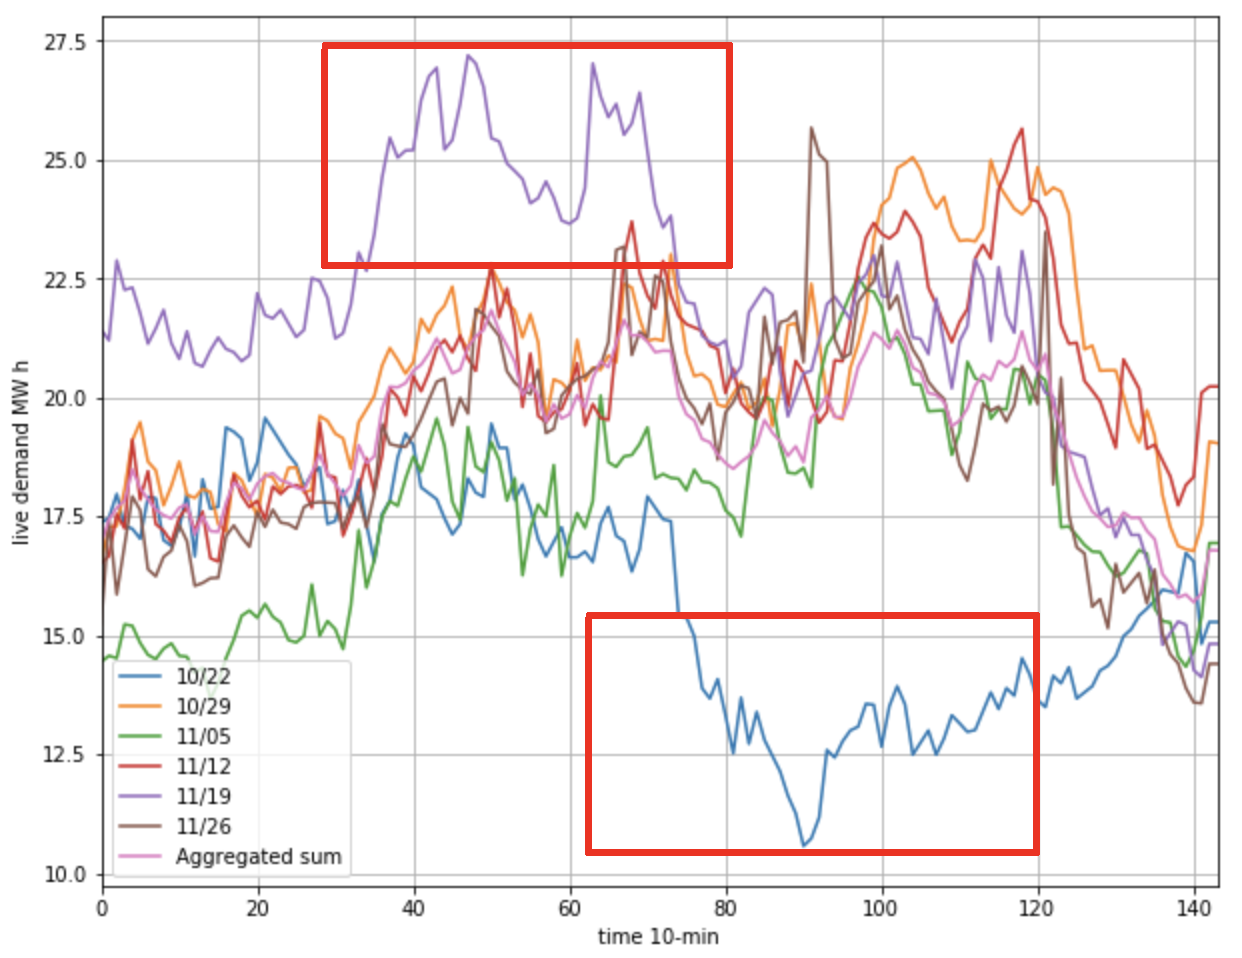
\includegraphics[scale=0.27]{monday_demand}}
                    \caption{The demand of mondays and their aggregated sum in one-day period, the differences of two outliers are specially selected}
                \end{figure}

                There should be reasons to explain the abnormal pattern on 10-22 and 11-19, however, no valid news or information can be found through web on these two days in Orkney. There must be something happen, for example, a maintenance which results in a lot of households turning off the appliances or a festival which increase the demand. Because 10-22 has lower average demand and 11-19 has larger average demand, and both of the days have larger standard deviations. The details of means and standard deviations are shown in Table \ref{table_mean_std_monday}.It should be viable to infer the two special conditions.

                \begin{table}[ht]
                    \label{table_mean_std_monday}
                    \centering
                    \begin{tabulary}{\linewidth}{c |c c c c c c c}
                        \hline
                         & 10-22 & 10-29 & 11-05 & 11-12 & 11-19 & 11-26 & Aggregation\\ \hline
                        % \hline
                        Mean & 15.82 & 20.68 & 17.67 & 20.31 & 21.83 & 19.05 & 19.23\\
                        Standard deviation & 2.31 & 2.18 & 2.18 & 2.09 &2.86 & 2.43 & 1.5\\
                        \hline
                    \end{tabulary}
                    \caption{Mean and standard deviation of six Mondays}
                \end{table}

                From Table \ref{table_demands_properties}, the average demand and the standard deviation in a global scope are 19.04 MW h and 2.92, and the four normal days have their means near to the global value, while the two outliers have larger differences. The aggregation data also has a closer average, the deviation is lower adhere to \emph{Variance} \footnote{For the sample average of i.i.d.:  $S_n = (X_1 + \dots + X_n)/n$, the deviation \\$\sigma_n^2 = \sigma^2/n$}.
                A more clean plot can be viewed in Figure \ref{plot_monday_agg}, where only the aggregated data and the mean is plotted. From the plot, it can be identified that there are four peak demand periods at almost the same level on the Monday, and they demonstrate the people's behaviors in the morning, noon, afternoon and evening.
                If 7:00 am - 8:00 pm (42 - 120 10-minute) is defined as the diurnal interval, most of consumption in this period will be over the mean consumption. Then the compliment of this period, the nocturnal period, has energy consumption lower than the average in most of the time.
                \begin{figure}[ht]
                    \centerline{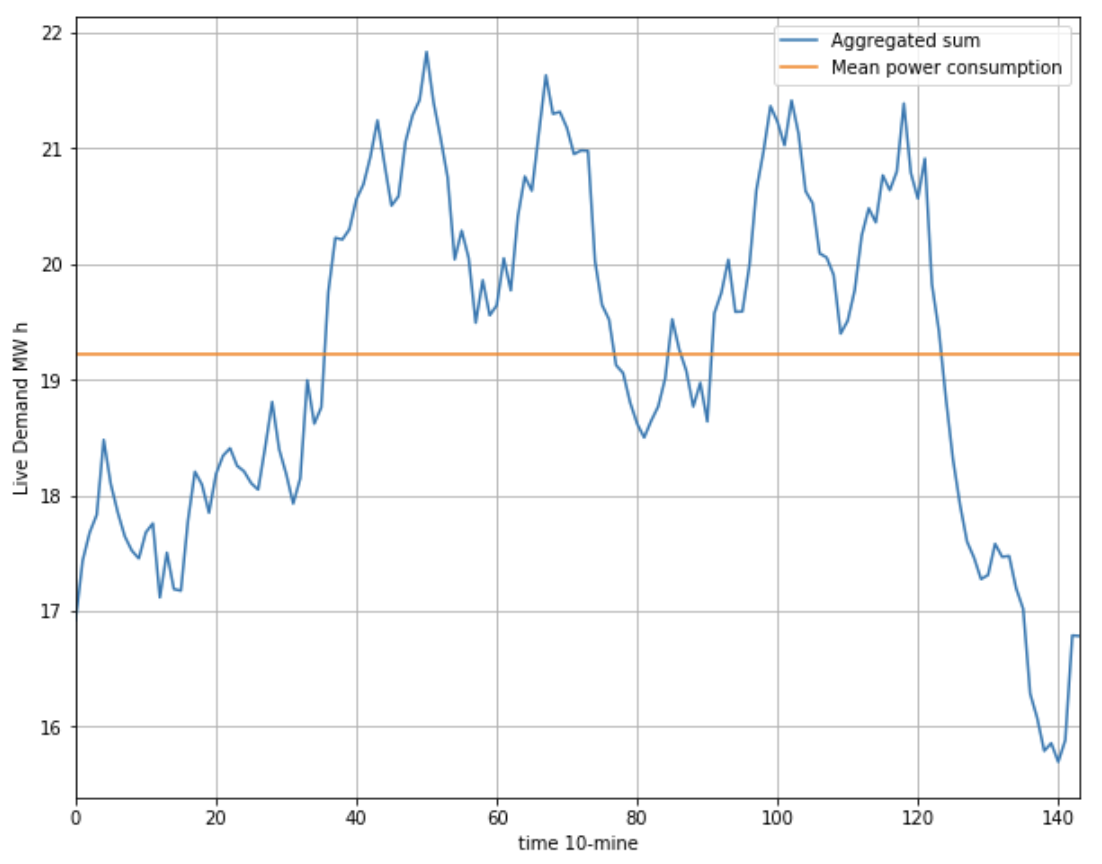
\includegraphics[scale=1.2]{monday_agg}}
                    \caption{The plot of Aggregation sum and its mean of Monday}
                    \label{plot_monday_agg}
                \end{figure}

                The next step is to apply this analysis method to each weekday. From the assumption and the experience of the Monday case, there will be some outliers in each weekday though, most weekdays appear a similar pattern and they are indicating the main tendency of demand. The date range is selected to be the whole November, as the data set was established at 19th October, and there are long term data loss in December and January \ref{text_source_stability}. The data is first classified by seven weekdays, then apply aggregation to each weekday group. Finally, the seven aggregation weekdays are plotted and analyzed to find their similar patterns.

                \begin{table}[ht]
                    \centering
                    \begin{tabulary}{\linewidth}{c |c c c c c c c}
                        \hline
                         & Sunday & Monday & Tuesday & Wednesday & Thursday & Friday & Saturday \\ \hline
                        % \hline
                        Sunday & 1 & 0.96 & 0.93 & 0.93 & 0.98 & 0.94 & 0.84 \\
                        Monday & 0.96 & 1 & 0.97 & 0.94 & 0.94 & 0.90 & 0.80 \\
                        Tuesday & 0.93 & 0.97 & 1 & 0.95 & 0.93 & 0.90 & 0.79 \\
                        Wednesday & 0.93 & 0.94 & 0.95 & 1 & 0.93 & 0.90 & 0.81 \\
                        Thursday & 0.98 & 0.94 & 0.93 & 0.93 & 1 & 0.92 & 0.81 \\
                        Friday & 0.94 & 0.90 & 0.90 & 0.90 & 0.92 & 1 & 0.95 \\
                        Saturday & 0.84 & 0.80 & 0.79 & 0.81 & 0.81 & 0.95 & 1 \\
                        \hline
                    \end{tabulary}
                    \caption{Correlation matrix of weekdays' aggregation on November Live demand}
                    \label{table_corr_weekday_demand}
                \end{table}

                Table \ref{table_corr_weekday_demand} shows the correlation matrix of the seven aggregations. As most of them are over 0.9, the profile of each weekday appears to be similar in large degree and it implies that they can be aggregated for the second time to form a new aggregation of the month. What can be verified is that the demand pattern of a day in Orkney is always following a similar pattern, the value may at a degree though, the peak value and the lowest value can always occur at the same time. This result should be implicitly true before the experiment, as this is the overall demand data, which records the total electricity demand of the island to represents the behavior of most people in common.
                
                \begin{figure}[ht]
                    \centerline{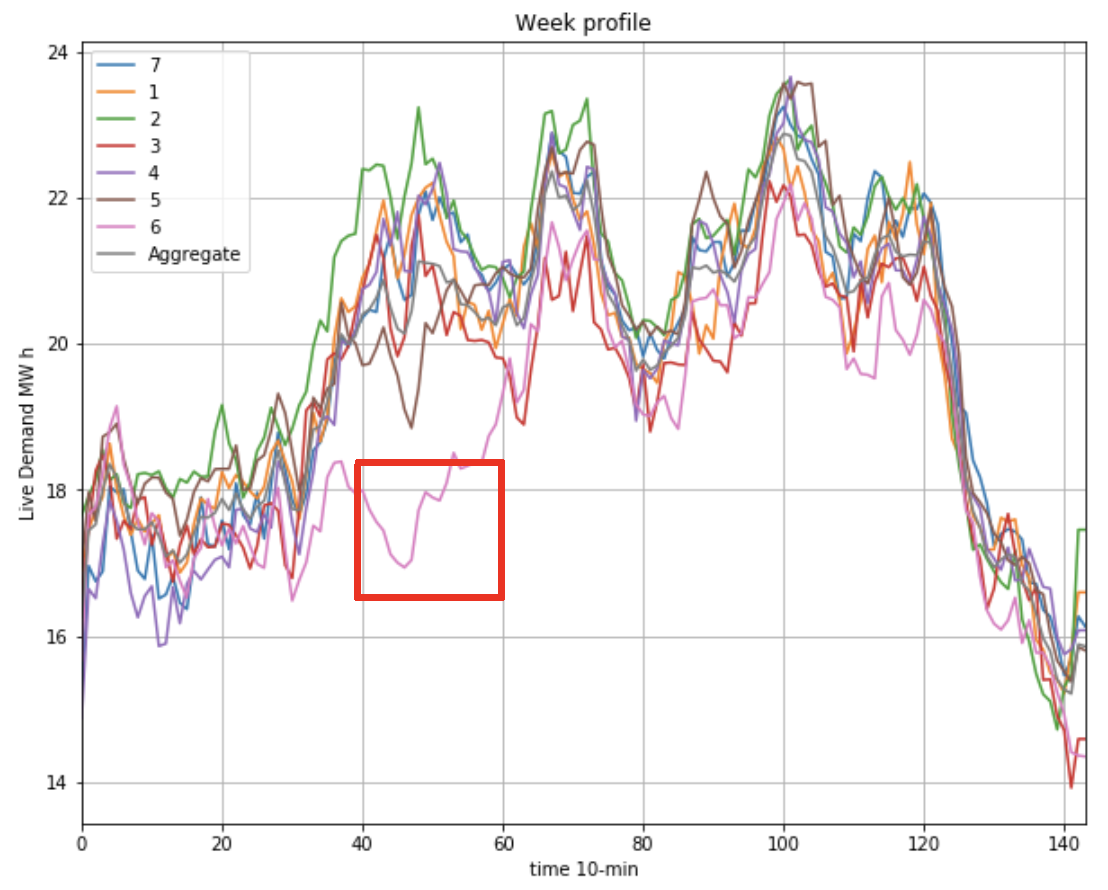
\includegraphics[scale=1.4]{weekday_profile}}
                    \caption{The aggregations of demand in 7 weekdays of November and the aggregation of the month}
                    \label{plot_week_profile}
                \end{figure}
                
                Figure \ref{plot_week_profile} shows a plot of the seven aggregation data to visualize their similarity. A discrepancy of them is at the red colored rectangle, where the demand of Saturday in the morning is lower. it can be verified from the correlation matrix that the scores for Saturday (at the bottom row) is lower about 0.1 than those of other weekdays on average. Except this disagreement, other aggregations appear to be largely similar and seem to follow the same path of growing and decaying during a day period. The aggregation of these seven weekday profiles is thus following the same pattern of the day.

                \subsection{Constructing Month profile}

                As it is mentioned in the last section, a profile of the month can be made using the aggregation of each weekday which is actually the aggregation of each day in the month. The reason is that the results of the aggregations of each weekday appear highly correlated, so that a new aggregation can be calculated based on this result. Apart from the behaviors in a day definition, the behaviors in a season definition can differ in various ways. The most general case is the heat is the heating consumption which is approximately zero in the summer but has a large load profile in the winter. \hyperref[plot_heating_season_effect]{Figure \ref*{plot_heating_season_effect}} shows the seasonal effect on heating appliances which is collected from \cite{report:household}. The factor can reach about 3.0 in January and drop to 0 in summer months, thus causing big variances for month profiles in different seasons.

                \begin{figure}[ht]
                    \centerline{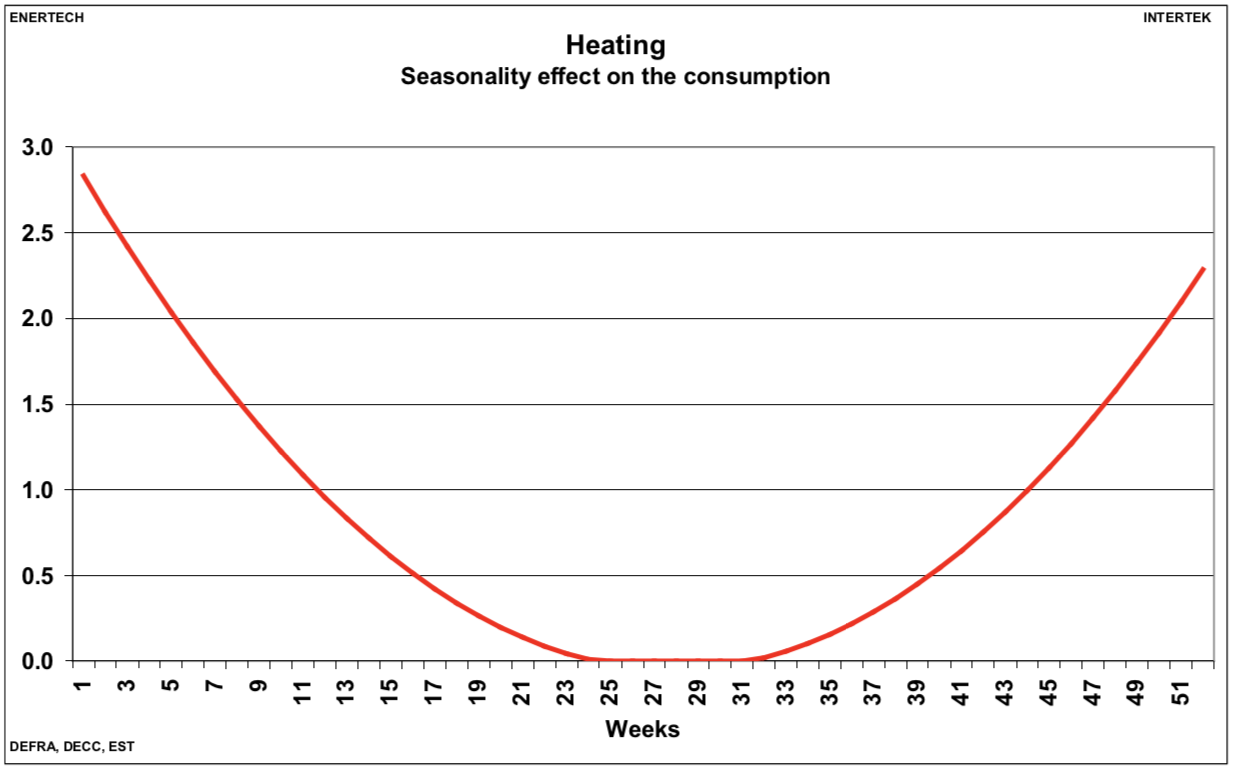
\includegraphics[scale=1]{heating_season_effect}}
                    \caption{Seasonal effect of heating}
                    \label{plot_heating_season_effect}
                \end{figure}

                \subsection{Analyzing the month profile of November}
                    Limited by the coverage of data set that it is collected in late October and huge corruptions happened in December and January (in \hyperref[text_source_stability]{Section \ref*{text_source_stability}}), the current available month profile analysis can only be applied to November. Additionally, the overview of this month has been enough for later analysis on the effects of EVs.
                    \hyperref[plot_november_demand_profile]{Figure \ref*{plot_november_demand_profile}} shows the final aggregation demand profile of November with three constant patterns: 21.9, 20.2, 17.7.

                    \begin{figure}[ht]
                        \centerline{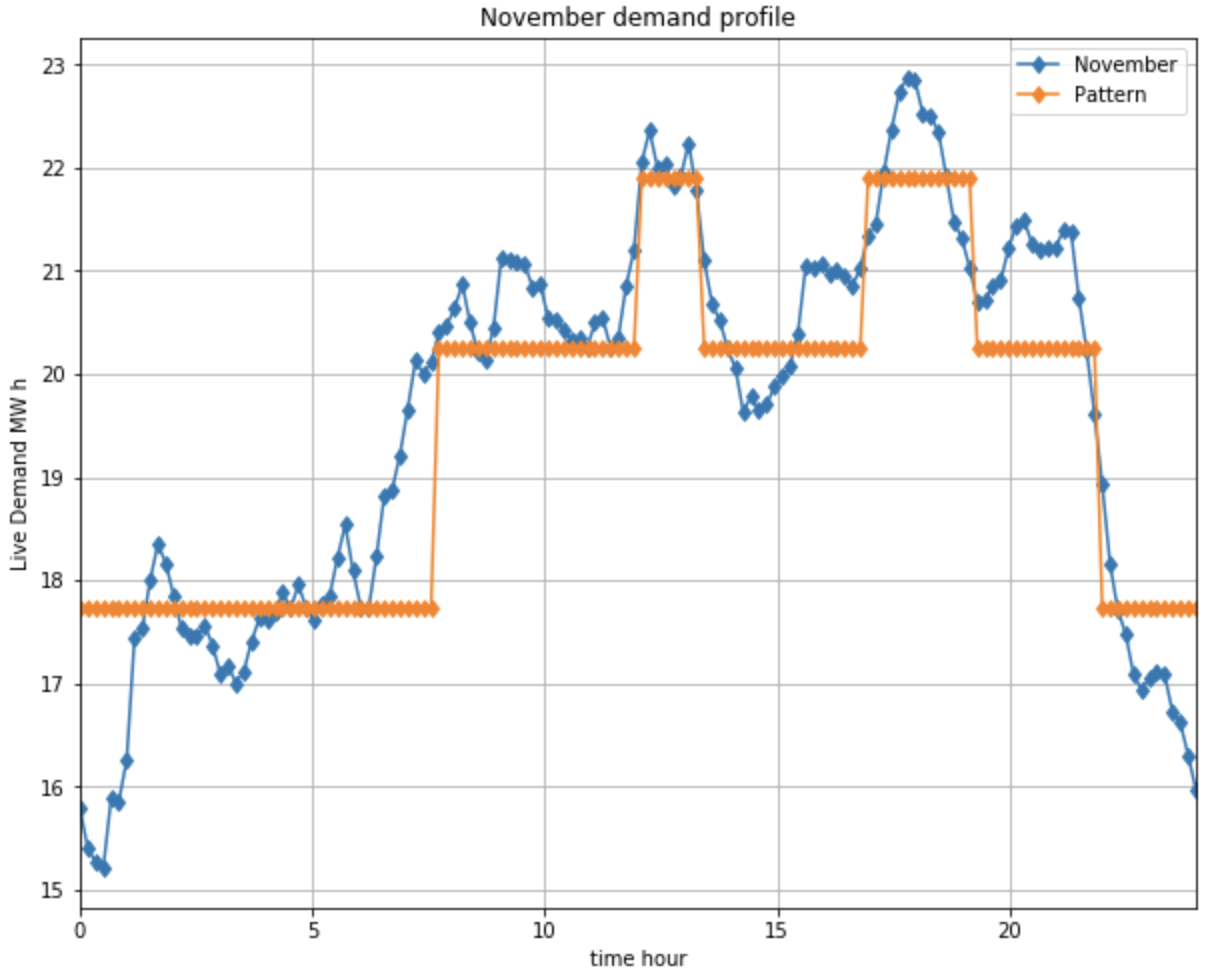
\includegraphics[scale=1]{november_demand_profile}}
                        \caption{The aggregated demand profile of November}
                        \label{plot_november_demand_profile}
                    \end{figure}
                
        \section{Analyzing Orkney Wind generation}
        The wind power generation analysis is fundamental to this project of building a generation-to-demand model. This analysis will provide statistical wind power characteristics and real-time cases for later simulation. In this section, the ANM record of wind power generation is first discussed, then a linear regression model will be created to link wind speed with wind power generation with curtailment introduced.

                \subsection{Analyzing the power generation attributes}
                As it has been mentioned in \hyperref[text_generation_and_demand_data_source]{Section \ref*{text_generation_and_demand_data_source}}, there are three attributes relating to the power generation: Orkney ANM, Non-ANM Renewable Generation, Total renewable capacity. The Orkney ANM is indicating the power generation from ANM system, and the Non-ANM Renewable Generation is the generation which is not controlled by ANM. As it is recorded in \cite{report:OrkneyAudit}, there are three kinds of \\connections of generation to grid. The Total renewable capacity should be the estimated full load generation at current time from its literal meaning. Adding the first two attributes as the Total generation to compare to the capacity by statistical characteristics. \hyperref[table_statistical_characteristics_generation]{Table \ref*{table_statistical_characteristics_generation}} shows their statistical characteristics, where Total \\Generation has the same standard deviation as Total Renewable Capacity, implying that they are vibrating at the same amplitude. This condition is similar to \hyperref[text_attributs_of_demand]{Section \ref*{text_attributs_of_demand}}, where the Peak Winter Demand and Live Demand can be added up to a constant at each point. Thus, the sum and subtraction of Total Generation and Total Renewable Capacity are performed as the Sum and Subtraction attributes in the table. As previously inferred, their sum appears to be a constant again. It is preposterous that the ANM choose to use these two attributes which can always be calculated from others, nor are their names misleading the readers.
                \begin{table}[ht]
                    \centering
                    % using @{\hspace{0.09\linewidth}} to change width of the column
                    % finally choose to use p attributes to coordinate manually
                    \begin{tabulary}{\linewidth}{c p{1.7cm} p{2cm} p{2cm} p{2cm} p{1.1cm} L}
                        \hline
                         & Orkney ANM & Non-ANM Renewable Generation & Total Generation & Total Renewable Capacity & Sum & Sub \\ \hline
                        % \hline
                        mean & 10.09 & 12.43 & 22.52 & 34.58 & 12.07 & 57.1 \\
                        std & 6.92 & 6.99 & 13.54 & 13.54 & 27.08 & 0 \\
                        min & -2.09 & 0.26 & -1.53 & 15.08 & -26.95 & 57.1 \\
                        25\% & 2.89 & 5.40 & 8.32 & 22.25 & -12.61 & 57.1 \\
                        50\% & 11.23 & 14.73 & 27.25 & 29.85 & 2.61 & 57.1 \\
                        75\% & 16.54 & 18.47 & 34.85 & 48.78 & 40.46 & 57.1 \\
                        max & 21.26 & 25.96 & 42.02 & 58.63 & 60.17 & 57.1 \\
                        \hline
                    \end{tabulary}
                    \caption{Statistical characteristics of Generation attributes}
                    \label{table_statistical_characteristics_generation}
                \end{table}

                Originally, another explanation is assumed that the Total Renewable Capacity attribute is the estimation of the available capacity of storage to the grid. There are two reasons to refute this position. One is that the ANM network has been commissioning no battery storage since 2015 and the only available storage is the hydrogen fuel installed by \emph{Surf`n'Turf} \cite{report:OrkneyAudit}. The other reason is that the storage should be represented by energy not power and even if it is represented using power, the mean, which is 15.07 from \hyperref[table_statistical_characteristics_generation]{Table \ref*{table_statistical_characteristics_generation}}, is not reasonable. Because the wind is strong in Orkney and there is 61\% of the time the generation is higher than the demand. This implies that the battery should be at approximately full storage for most of the time. Having proved that Total Renewable Capacity is of nonsense, the two renewable generation attributes are applied to an additive operation on element wise to form a Total Generation attribute, as they are both renewable generations installed by different sponsors.

                \subsection{Analyzing the weather attributes}
                \label{text_wind_speed_analysis}
                As it is discussed in \hyperref[text_weather_data_source]{Section \ref*{text_weather_data_source}} that wind speed, temperature and humidity attributes are recorded in the data set, a first attempt is on the wind speed for its strong relation to wind power generation.
                \hyperref[table_wind_speed_characteristics]{Table \ref*{table_wind_speed_characteristics}} shows the wind speed characteristics. Though the average speed is 6.01 m/s, the max value can reach 19.5 m/s,
                which must be identified as extreme weather. The 50 percentiles reach only 5.7 m/s, indicating that about half of the days have smaller wind speed than the average. However, the 75 percentiles construct
                a strong wind group with larger deviation than other intervals, implying the various conditions of wind, which result in challenges for the wind generation.

                \begin{table}[ht]
                    \centering
                    \begin{tabulary}{\linewidth}{C C C C C C C}
                        \hline
                        Mean & Std & Min & 25\% & 50\% & 75\% & Max \\ \hline
                        % \hline
                        6.01 & 3.42 & 0.5 & 3.1 & 5.7 & 8.2 & 19.5 \\
                        \hline
                    \end{tabulary}
                    \caption{Wind speed statistical characteristics}
                    \label{table_wind_speed_characteristics}
                \end{table}

                Another special scenario of wind speed is its distribution. From the data of Orkney, the mean of is more near to the min than the max. If it is subtracted by two standard deviation, it will be a minus value and it is impossible. While the adding of two standard deviation is possible and it results in at least 75 percentiles, which is adhere to \emph{Chebyshev's Inequality} \footnote{In probability theory, Chebyshev's inequality also called the Bienaymé–Chebyshev inequality) guarantees that, for a wide class of probability distributions, no more than a certain fraction of values can be more than a certain distance from the mean. \\ $\Pr(|X-\mu| \ge k \sigma) \le \frac{1}{k^2}$ \cite{website:chebyshev}} to be smaller than 0.25.
                The distribution is \emph{Weibull distribution} \cite{paper:windstructure}, which is a modified version of the general \emph{Rayleigh distribution}.

                \subsection{Analyzing the curtailment attributes}
                The curtailment data is collected as binary type in \hyperref[text_fetching_curtailment_data]{Section \ref*{text_fetching_curtailment_data}}. There are three kinds of issues in a zone: ANM Operation, SHEPD Equipment, Generator Site Issue. For the sake of simplicity, the curtailment of one zone is the result of any issues in the zone.

                \subsection{Linking wind power generation to wind speed and curtailment}
                The difficulty of this problem is that the influence of the other attribute cannot be removed while analyzing one attribute. For example, the wind power increases along with the growth of wind speed, it then reaches a maximum limited by the largest rotation speed of the wind turbines. Thus, the model of generation should first increase linearly with wind speed, then appears horizontally at higher wind speed. With the addition of curtailment, the model reaches the maximum level earlier and even the generation with lower wind speed is affected, as the curtailments happen whenever the generation exceeds the demand to some degree.
                It is thus possible to make a regression model which is allowed to under-estimate the generation.
                \label{text_wind_regression_model}
                    \subsubsection{Choosing and Analyzing the sample data}
                    It is deeply acknowledged that the data matters more than algorithms in machine learning, which is discussed in \cite{paper:datasize}. However, the data size of this model is just from one day which is specifically selected to demonstrate the main feature of wind speed to generation.
                    As it is depicted in \hyperref[plot_speed_vs_power_1202]{Figure \ref*{plot_speed_vs_power_1202}} that 12-02 is selected as the sample source. The reason is that an apparent linear relation of wind speed to generation and the upper limitation can be detected in the figure.
                    It can be found that the the generation grows linearly reciprocal to the wind speed before the wind speed reaches 8 m/s. Then it stops at about 38 WM h. The red line in the figure depicts the expected generation characteristics.

                    \begin{figure}[ht]
                        \centerline{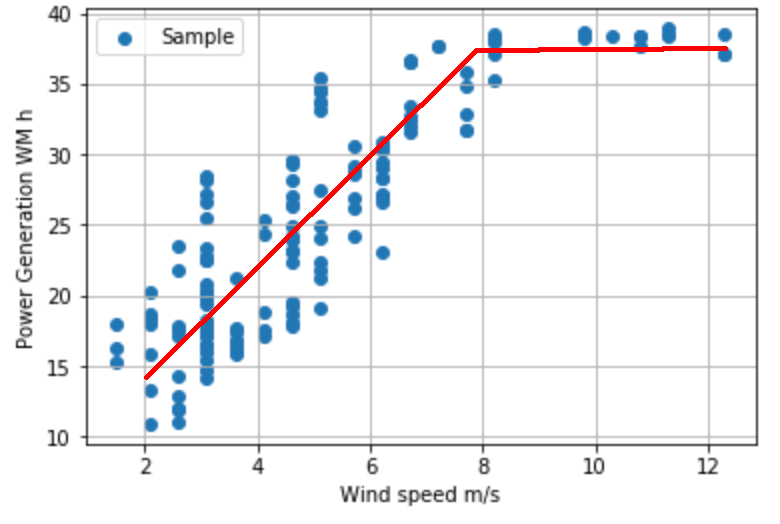
\includegraphics[scale=1.4]{powervsgenerationsample}}
                        \caption{The wind speed versus power generation on 12-02}
                        \label{plot_speed_vs_power_1202}
                    \end{figure}

                    \begin{figure}[ht]
                        \centerline{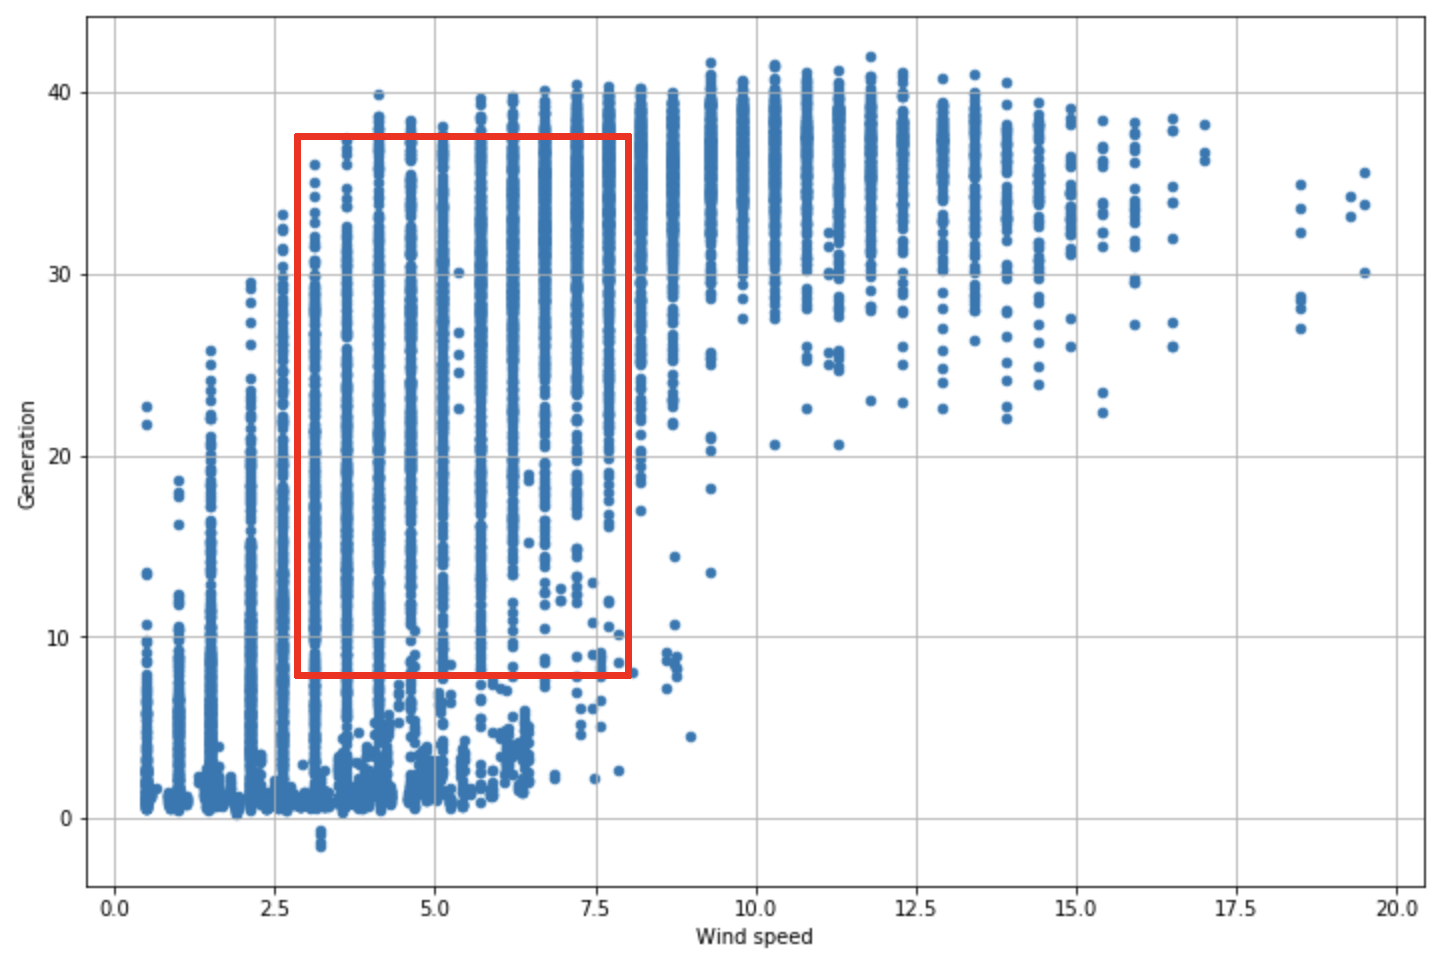
\includegraphics[scale=0.2]{generationvsspeedwholeset}}
                        \caption{The wind speed versus power generation on the whole data set}
                        \label{plot_speed_vs_power_whole}
                    \end{figure}
                
                    If the whole data set is selected, as \hyperref[plot_speed_vs_power_whole]{Figure \ref*{plot_speed_vs_power_whole}} indicated, various curtailment conditions will definitely affect the model. As the red colored rectangle emphasized, the value generation of 2.5 m/s to 7.5 m/s has approximately the same range of value which cannot be appropriately understood by the algorithms.

                    \subsubsection{Modeling the relation of wind speed and power generation}
                    Two linear regression methods are tested on this relation: linear regression, and polynomial linear regression. As the red line shows, the linear regression of the first order should be separated into two regions. The case for the second order linear regression is easy to apply on the whole wind speed interval.

                    
                    The resultant parameters of two regression models along with their Mean squared error are shown in \hyperref[table_two_model]{Table \ref*{table_two_model}}. These two regression strategies both result in an acceptable \textbf{MSE}, thus it is appropriate to use both of them to predict wind power generation from the speed.

                    \begin{table}[ht]
                        \centering
                        \begin{tabulary}{\linewidth}{|C C C C C|}
                            \hline
                            model & intercept & $a_1$ & $a_2$ & MSE\\ \hline
                            linear & $7.5$ & $3.75$ & $0$ & $14.4$ \\ \hline
                            polynomial & $5.1$ & $5.22$ & $-0.19$ &  $15.05$ \\
                            \hline
                        \end{tabulary}
                        \caption{Parameters of two linear regression model on wind speed to power generation on 12-02}
                        \label{table_two_model}
                    \end{table}

                    It should be noted that the reason why the conditions happen in the rectangle region of \hyperref[plot_speed_vs_power_whole]{Figure \ref*{plot_speed_vs_power_whole}} is that the curtailment occurs whenever the demand cannot fully follow the generation capacity to sustain the stability of the grid.
                    
                    \subsubsection{Modeling the relation of curtailment and power generation}
                    Under the condition that the demand is enough large that no curtailment occurs, the wind speed-to-generation model derived in the previous section is approximating the power generation well. However, according to statistics of last few years, the time of curtailment takes up to 31\% of all time periods. Another model modeling the generation under curtailment should be added to include all conditions in the wind power generation model.

                    The assumption is that, when the curtailment happens, some wind turbines are cut out, causing the power generation being limited to a level slightly above the demand.
                    This assumption is expressed as:
                    \begin{equation}
                        Generation \leq Live Demand + k
                        \label{equation_Generation_to_demand_curtailment}
                    \end{equation}
                    The crux is to find the optimal value of $k$. Using the wind speed-to-generation model to predict the power generation of the full capacity, then add $k$ to the current demand. If the generalization is higher than this value, this time slot will be marked as curtailment happen. Comparing the predictions of curtailment with the collected ANM status data using the \emph{Confusion matrix} in \hyperref[table_error_types]{Section \ref*{table_error_types}}.
                    To acquire the value $k$ which fits in a general scenario, the curtailment data of nine regions is transformed into a single boolean value which is true if at least two regions have reported curtailment. The linear speed-to-generation model is the polynomial model, and the values of $k$ range from 1 to 20.

                    \begin{table}[ht]
                        \centering
                        \begin{tabulary}{\linewidth}{C C C C C C C C C C C}
                            \hline
                            k & 1 & 2 & 3 & 4 & 5 & 6 & 7 & 8 & 9 & 10\\ \hline
                            Type I
                            & 0.02 & 0.03 & 0.04 & 0.05 & 0.06 & 0.07 & 0.08 & 0.11 & 0.13 & 0.18\\ \hline
                            Type II
                            & 0.53 & 0.50 & 0.46 & 0.41 & 0.37 & 0.34 & 0.31 & 0.25 & 0.20 & 0.17\\ \hline
                            k & 11 & 12 & 13 & 14 & 15 & 16 & 17 & 18 & 19 & 20\\ \hline
                            Type I
                            & 0.22 & 0.28 & 0.35 & 0.42 & 0.52 & 0.60 & 0.68 & 0.74 & 0.79 & 0.86\\ \hline
                            Type II
                            & 0.14 & 0.11 & 0.09 & 0.07 & 0.05 & 0.05 & 0.04 & 0.02 & 0.02 & 0.01\\ \hline
                        \end{tabulary}
                        \caption{Type errors of parameter $k$}
                        \label{table_type_error_k}
                    \end{table}
                    \hyperref[table_type_error_k]{Table \ref*{table_type_error_k}} shows the scores of this binomial regression model. The performance is relatively high \footnote{By taking the average of the two type error for each k or the weighted sum of them, as the target is to predict the occurrence of curtailment, not the normal mode.} when $k = 8,9,10$. Taking the median of them and the model is constructed as:
                    \begin{equation}
                        Generation \leq Live Demand + 9
                    \end{equation}


            \section{Modeling the over-all EV effects}
            To analyze the demand of EVs, it is necessary to first construct the model of demand, then it can be synthesized with the Live demand model derived in the previous section. 

            As it is elaborated in \hyperref[text_EV_charging_profile]{Section \ref*{text_EV_charging_profile}} that the demand of EVs to the grid is determined by the charging station type and the capacity of batteries. Besides the power approximation, the demand in time-series should be characterized using the charging events model, which is statistically fitting to the histogram of arrivals and departures in \hyperref[fig_arrival_vs_departure]{Figure \ref*{fig_arrival_vs_departure}}.

            In this section, the charging events model is first designed. It is fundamentally necessary to the model of demand of EVs and the implementation of simulating EV charging. Then, the effects of different penetration levels of EVs will be analyzed.

                \subsection{Characterizing EV charging events}
                \label{text_ev_charging_model}
                To characterize the charging events of EVs, several presumptions are first promoted: (1) All of the EVs are charged only one time each day, and they are charged equivalent amount of energy. (2) Only one type of EV is considered to unify the capacity of batteries. (3) Bidirectional power transportation technologies: V2G, V2H, and V2V \cite{paper:v2g}, are not considered to decrease the degree of complexity.

                From \hyperref[fig_arrival_vs_departure]{Figure \ref*{fig_arrival_vs_departure}}, it seems that there are two peak arrival time each day: 12:00 and 18:00, and the latter is larger. The first distribution is extracted from \cite{paper:Shao2010}, which uses a normal distribution with $\mu = 18:00, \sigma = 1$, implying that the peak time is at 18:00, and most EVs arrive in the range $15:00 - 21:00$ \footnote{The interval is 3 standard deviations of the mean, which covers 99.7\% of the data \cite{website:normaldistribution}. Actually, $\sigma$ can be slightly larger as there are still arrivals after 22:00.}.
                Using the random number generation module of \emph{Numpy}, it is possible to produce a set of charging start points with the number of EVs provided. \hyperref[fig_normal_histogram]{Figure \ref*{fig_normal_histogram}} shows a histogram of samples in this distribution.

                \begin{figure}[ht]
                    \centerline{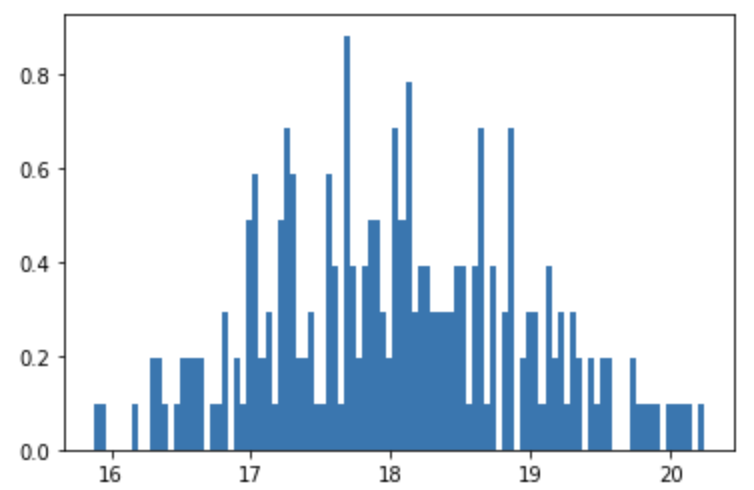
\includegraphics[scale=1.3]{normalHistogram}}
                    \caption{The Histogram of the samples generated by a Normal distribution of $\mu = 18, \sigma = 1$}
                    \label{fig_normal_histogram}
                \end{figure}

                There are 234 EVs in Orkney (\hyperref[table_current_condition_of_EVs]{Table \ref*{table_current_condition_of_EVs}}), and the total daily demand can be calculated: $ W_{perday} = 21.74 * 0.299 = 6.5 kW h$. Two charging modes are considered in this scenario: 110V/15A * 5.5h as the Normal charging, and 240V/30V * 1.5h as the quick charging.
                Under such condition, the demand caused by the charging events can be visualized in \hyperref[fig_charging_demand_234]{Figure \ref*{fig_charging_demand_234}}. The differences on instant charging power and length of charging periods lead to significant demand profiles of the two modes. The peak value of Quick charging is over 2 times higher than that of the normal charging mode and the peak value reaches about 2 hours earlier than the Normal charging mode \footnote{It also implies a possible solution to delay the demand peak time by transform Quick charging to normal charging.}.

                \begin{figure}[ht]
                    \centerline{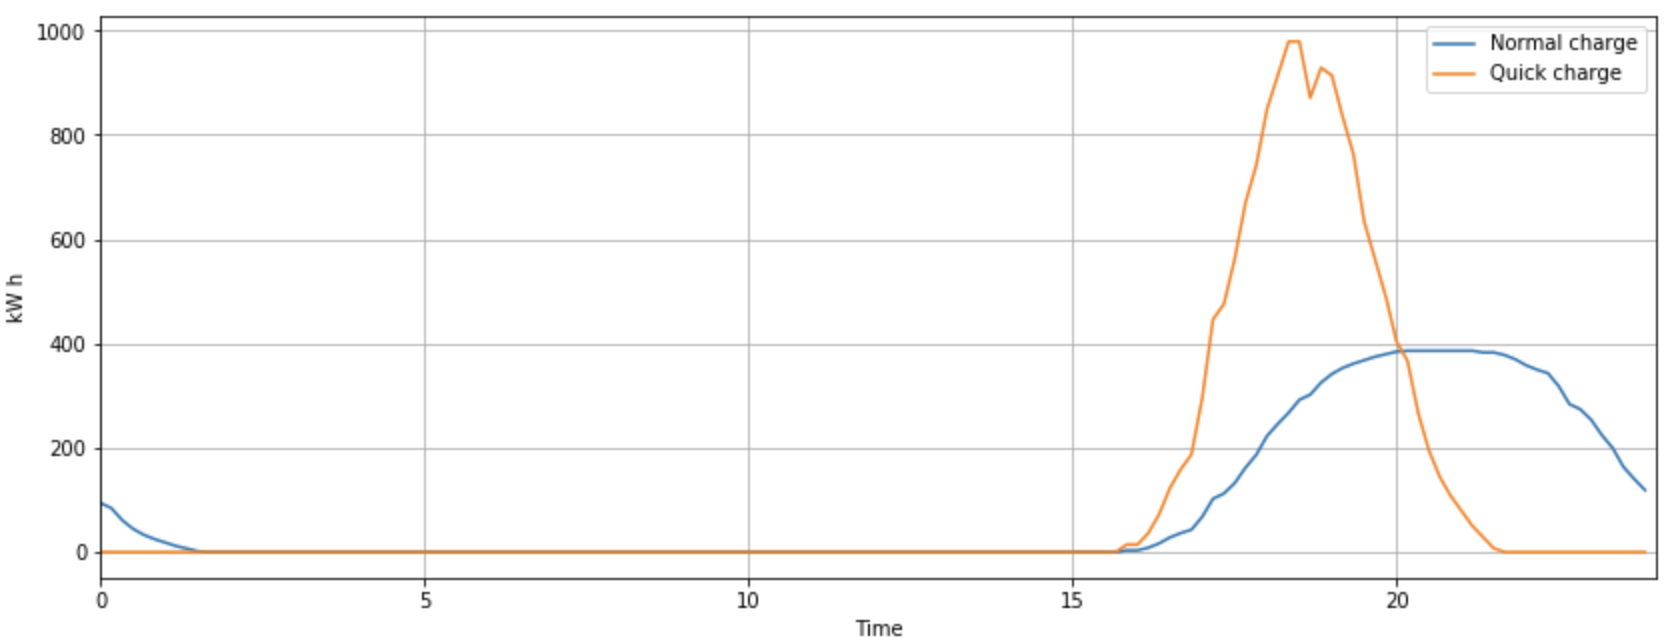
\includegraphics[scale=1]{chargiingEventsOriginPenetration}}
                    \caption{The demand profile of 234 EVs under two charging mode}
                    \label{fig_charging_demand_234}
                \end{figure}

                Despite the demand profile derived from one peak time, a more pragmatic approximation can be constructed by two normal distributions centering at 12:00 and 18:00, respectively. The idea behind the choice of these two center point is to achieve a replica of the Arrivals vs Departure Histogram in \hyperref[fig_arrival_vs_departure]{Figure \ref*{fig_arrival_vs_departure}}.

                The histogram of the charging events and the demand profile of this new approximation are demonstrated in \hyperref[fig_two_peak_histogram]{Figure \ref*{fig_two_peak_histogram}} and \hyperref[fig_charging_demand_234_2]{Figure \ref*{fig_charging_demand_234_2}}.
                \begin{figure}[ht]
                    \centerline{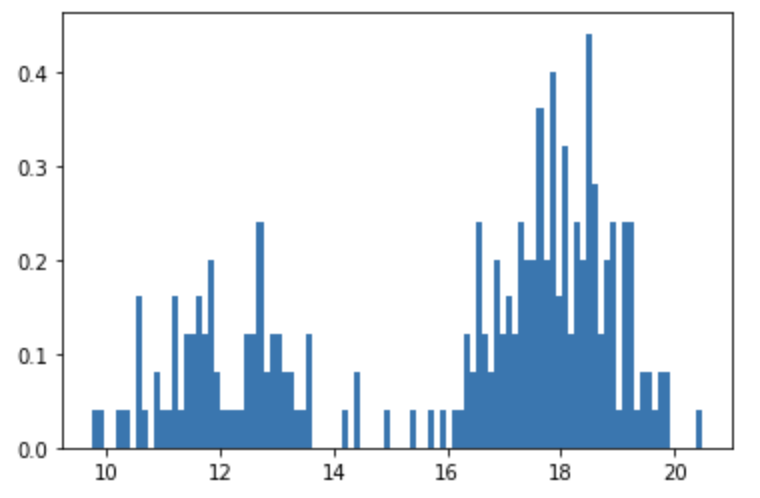
\includegraphics[scale=1.5]{twoPeakHist}}
                    \caption{The Histogram of the samples generated by two normal distributions at 12:00 and 18:00}
                    \label{fig_two_peak_histogram}
                \end{figure}

                \begin{figure}[ht]
                    \centerline{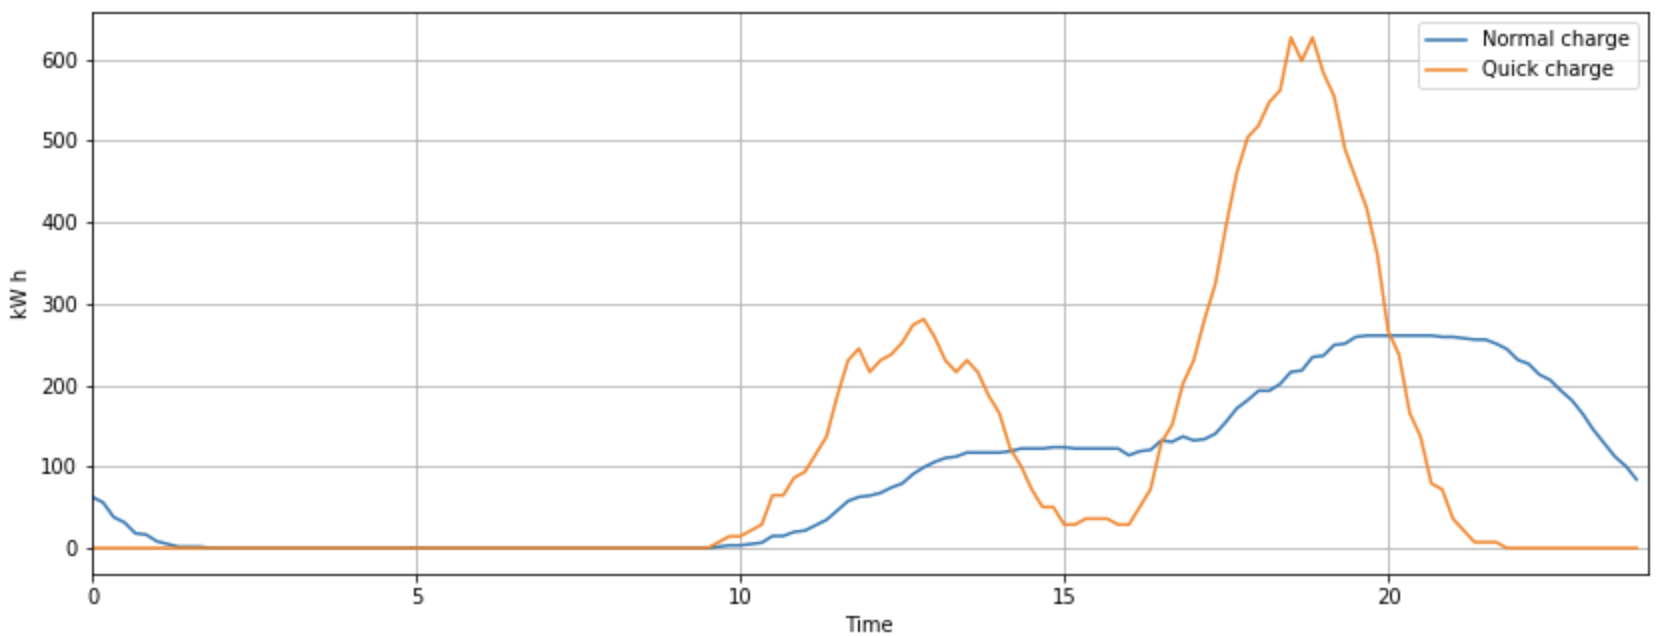
\includegraphics[scale=1]{chargingEventsTwoPeak}}
                    \caption{The demand profile of 234 EVs with two charging peak time}
                    \label{fig_charging_demand_234_2}
                \end{figure}

                \subsection{Analyzing different penetration levels}
                The current penetration level 1.4\% has not attached a threat to the grid. If all EVs are recharged in one day, the total consumption is $6.5 * 234 = 1521 kW h$, while the island total demand on a daily average is $469 MW h$. This little consumption can be visualized in \hyperref[fig_1.4_syn]{Figure \ref*{fig_1.4_syn}}, where merely a slight increase at night can be detected.

                \begin{figure}[ht]
                    \centerline{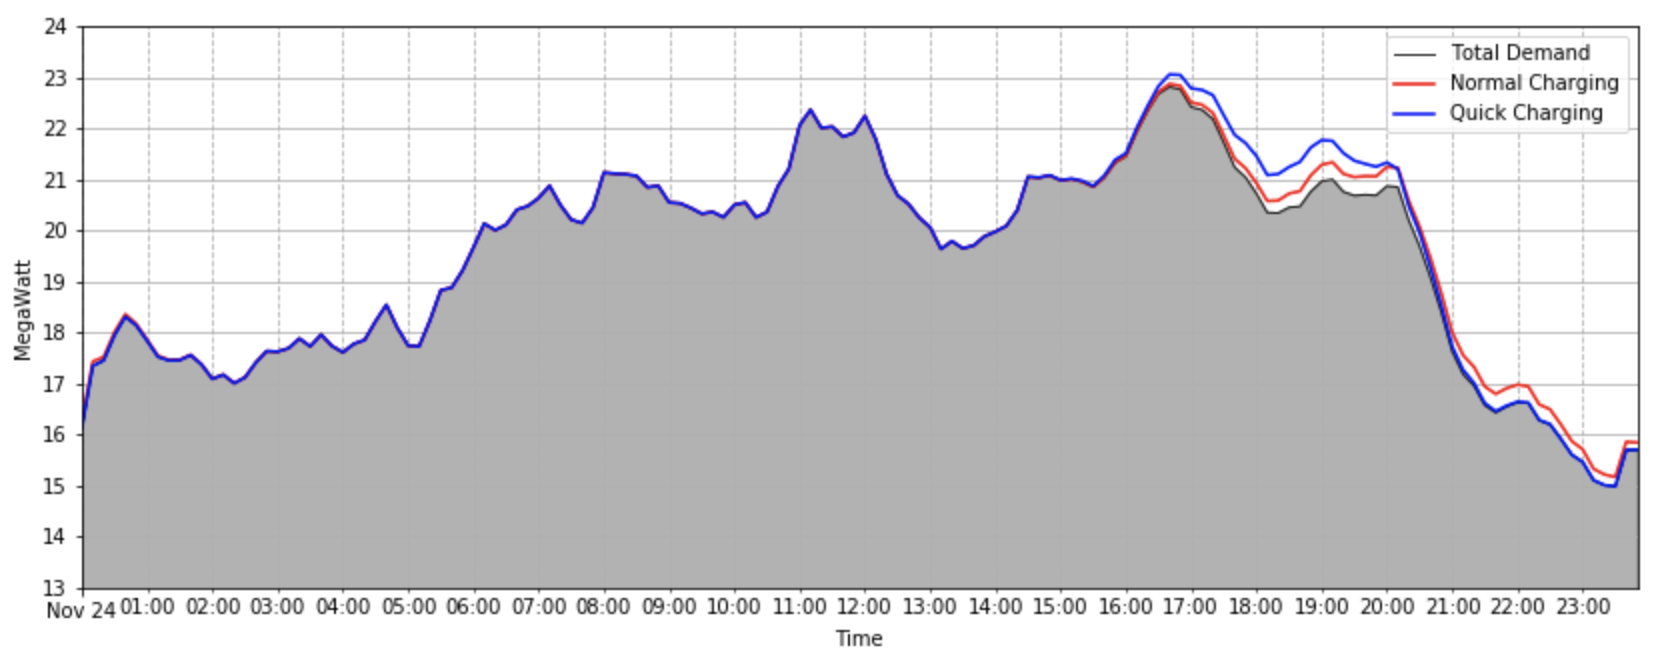
\includegraphics[scale=1]{currentsyn}}
                    \caption{The Synthesized demand profile of 1.4\% EV penetration}
                    \label{fig_1.4_syn}
                \end{figure}

                Comparing to the prediction of EV penetration in \cite{paper:Vazquez2010} that the percentage is 35\% in 2020, this penetration level is over-estimated.
                Three penetration levels: 10\%, 20\%, and 30\% are tested on current demand profile. \hyperref[table_demand_statistics_three_penetration_level]{Table \ref*{table_demand_statistics_three_penetration_level}} shows the results after adding the charging events at centering at 18:00.
                The scenario without EVs is also estimated by subtracting the 1.4\% EV consumption from the demand profile, then new penetrations are tested. During the process of increasing the penetration from 10\% to 30\%, the total energy demand, which can be estimated from the mean values, is increasing over 10\%, the max instant power consumption increases about 30\% for Normal charging and 80\% for Quick charging. The time is delayed to after 8 o'clock in the evening for Normal charging, and 6 o'clock in the evening for Quick charging.

                \begin{table}[ht]
                    \centering
                    \begin{tabulary}{\linewidth}{C C C C}
                        \hline
                         & Mean & Max & Peak Time \\ \hline
                        No EV & 19.6 & 22.88 & 15:40 \\ \hline
                        10\% (Normal) & 20.11 & 24.14 & 18:10 \\ \hline
                        10\% (Quick) & 20.23 & 28.91 & 18:20 \\ \hline
                        20\% (Normal) & 20.74 & 26.44 & 20:10 \\ \hline
                        20\% (Quick) & 20.98 & 34.7 & 18:20 \\ \hline
                        30\% (Normal) & 21.37 & 29.19 & 20:10 \\ \hline
                        30\% (Quick) & 21.73 & 41.36 & 20:10 \\ 
                        \hline
                    \end{tabulary}
                    \caption{The statistics of demand under three penetration levels}
                    \label{table_demand_statistics_three_penetration_level}
                \end{table}

                A more obvious impression is available by plotting the demand profile of the 30\% penetration in \hyperref[fig_penetration_30]{Figure \ref*{fig_penetration_30}}, where a single charging interval is too significant to accept as a rational estimation. The reason may be that the 30\% is impossible for current demand level, and it is also an estimation of maximum with all EVs using Quick charging mode, which implies that the real consumption should lie between the Quick mode and the Normal mode. Additionally, if the distribution of two peak times is considered, the peak value will be alleviated and the peak value will be distributed to two mountains on the graph.

                \begin{figure}[ht]
                    \centerline{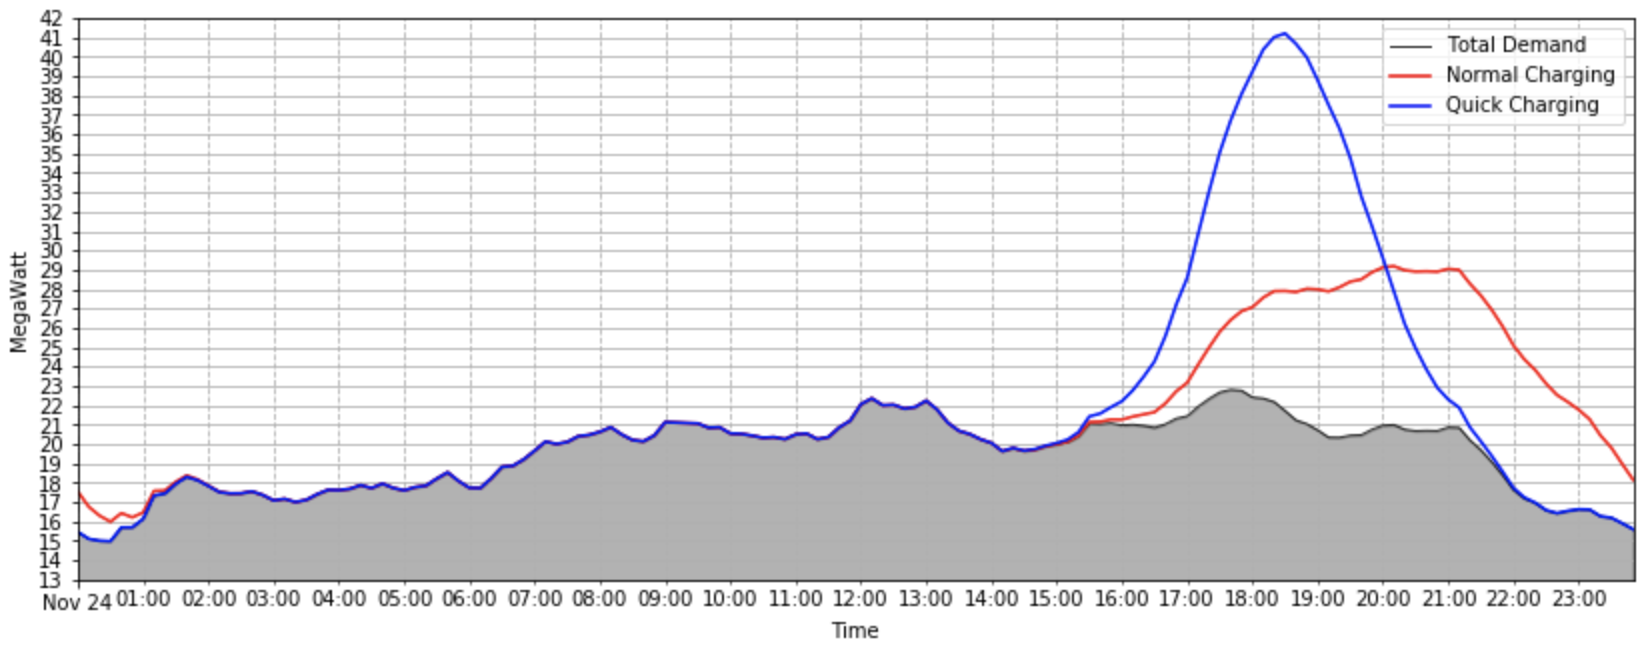
\includegraphics[scale=1]{penetration_30}}
                    \caption{The demand profile under the 30\% penetration of EVs}
                    \label{fig_penetration_30}
                \end{figure}
            
            \section{Implementing the simulation model of the grid}
            
            In this section, the details of the implementation of the simulation model are recorded. This simulation model is designed under the \emph{NASA Trick} simulation environment, which has been introduced in \hyperref[text_nasa_trick]{Section \ref*{text_nasa_trick}}. The whole grid model is separated into several independent models: household loading model, EV charing model, wind model, and storage model. The deliberate design of these parts makes it possible to simulate each single part without the couple of other elements, and it is better for unit test. Later these models are integrated into the whole grid model.
            
            Each model has four common methods: default, init, analytic, and terminate. The `default' method is called before `init' method to assign parameters to default value, the `init' method is called to initialize the state of some variables and manage memory blocks. These two methods are both called once at the start up of the simulation. The `analytic' method is called on every time slot to process the simulation, which means the number of times of calling this methods is equivalent to the number of time slots. The `terminate' method is called at the end of the simulation to summarize the result and clear applied memories.
            
            To exemplify, the household model identifies all appliances in the house, reads in the data of profiles of appliances, and creates variables for them in `default' method. Then, the `init' method is called to synchronize all appliances to the state of the same time and prepare other miscellaneous parameters for later analysis. The simulation control logic create the \emph{schema}, which stores the procedures on each time slots, and starts the timer. The `analytic' method updates the state of each appliance on each calling. If some data record processes are register, for example, the total energy consumption is recorded on every 10 minutes, and the consumption of light is recorded on every minute.
            When the \emph{schema} runs to the end, the `terminate' method is called, the mean and sum of the total consumption can be recorded in this method, and scores based on objective functions can be calculated, then the applied memory blocks are cleared to avoid memory leak.

                \subsection{Simulating Household load}
                \label{text_simulatinghouseholdload}
                The house contains various appliances which have specific characteristics, which have been summarized in \hyperref[table_electrical_devices]{Table \ref*{table_electrical_devices}}. There are 8 types of appliances considered in this model: refrigerator, cleaning, heating, cooking, lighting, audiovisual, computer, unknown. Among them, the cleaning, lighting, audiovisual, computer, and unknown are characterized using stochastic model, and others are based on periodic constants from their consumption profile.
                Because these appliances have different demand profiles, they are independently designed small models.
                The data of the consumption of appliances is based on \cite{report:household}, and the details are included in \hyperref[fig_all_app]{Figure \ref*{fig_all_app}}. The consumption profiles of specific appliance are also provided in the \hyperref[text_appendices]{Appendices}.

                \subsubsection{Simulating periodical appliances}
                The simulation of appliances which consume energy with predefined period is implemented by storing the data of a period in the model. As the time updates, the consumption of the appliance is adhere to the data at that time \footnote{Thus, a simple is implementation is to store the time-series data in to an array, each time the consumption is updated by reading the corresponding data by calculating the index}. 
                \subsubsection{Simulating stochastic appliances}
                It is known in \hyperref[text_household_loading_profile]{Section \ref*{text_household_loading_profile}} that the stochastic appliances can be classified into two group: randomly plug in with randomly working period, randomly plug in with fixed working period. For the former type, the time of plug in should be random and the working period should also be random, the later one is only random on the time of plug. 

                \begin{figure}[ht]
                    \centerline{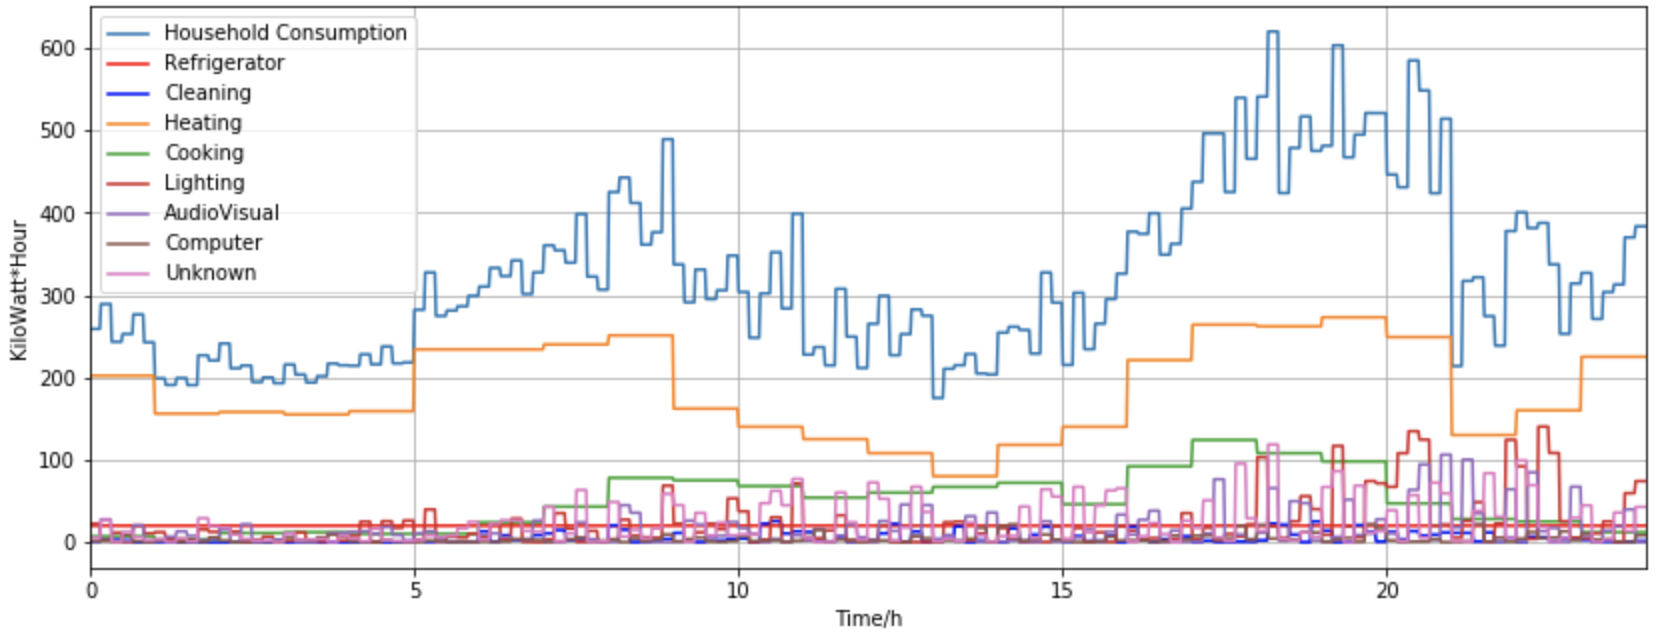
\includegraphics[scale=1]{simu_household}}
                    \caption{A one-day-interval simulation result of the household}
                    \label{fig_simu_household}
                \end{figure}

                \hyperref[fig_simu_household]{Figure \ref*{fig_simu_household}} shows the simulation result. Comparing to the source of data in \hyperref[fig_all_app]{Figure \ref*{fig_all_app}}, the simulation successfully recover the scenario of household consumption.
                \subsection{Simulating EV charging load}
                To simulate the charging process of electrical vehicles, two models are designed: EV, and charging station. The model of EV has attributes indicating the SoC, the time of arrival and departure, which use the statistical model derived in \hyperref[text_ev_charging_model]{Section \ref*{text_ev_charging_model}}. Each time the EV arrives at home, it is connected to the charging station, which controls the charging rate \footnote{As the strategies on charging should be tested later, it is necessary to abstract a layer between the grid and EV, the charging station, which communicates to the network and determines whether to charge the EV at the current time}.

                Three charging strategies are implemented in this charging station. The first is to charge the EV whenever it is connected to the charging station. The charging power is the normal mode: 110V/15A. The reason is that the charging station generally ignores the current state of the grid to complete the charging and the normal mode causes less instant power consumption to the grid. The second one is to delay the charging time to the late night, generally after 24:00, as it is the time interval that the demand of other appliances is at the lowest level. It is also using the normal mode charging power as this is a period of time that most EVs are charging together and the night gets enough time for them to be fully charged. The third strategy is based on a bi-directional communication channel, which makes it possible to let the charging station determine the charging power dynamically. In this strategy, the charging station predicts the expected departure time of the EV and determine whether to charge the car based on the current load of grid. Charing power is the quick mode as the smart strategy has the feedback from the grid.

                \begin{figure}[ht]
                    \centerline{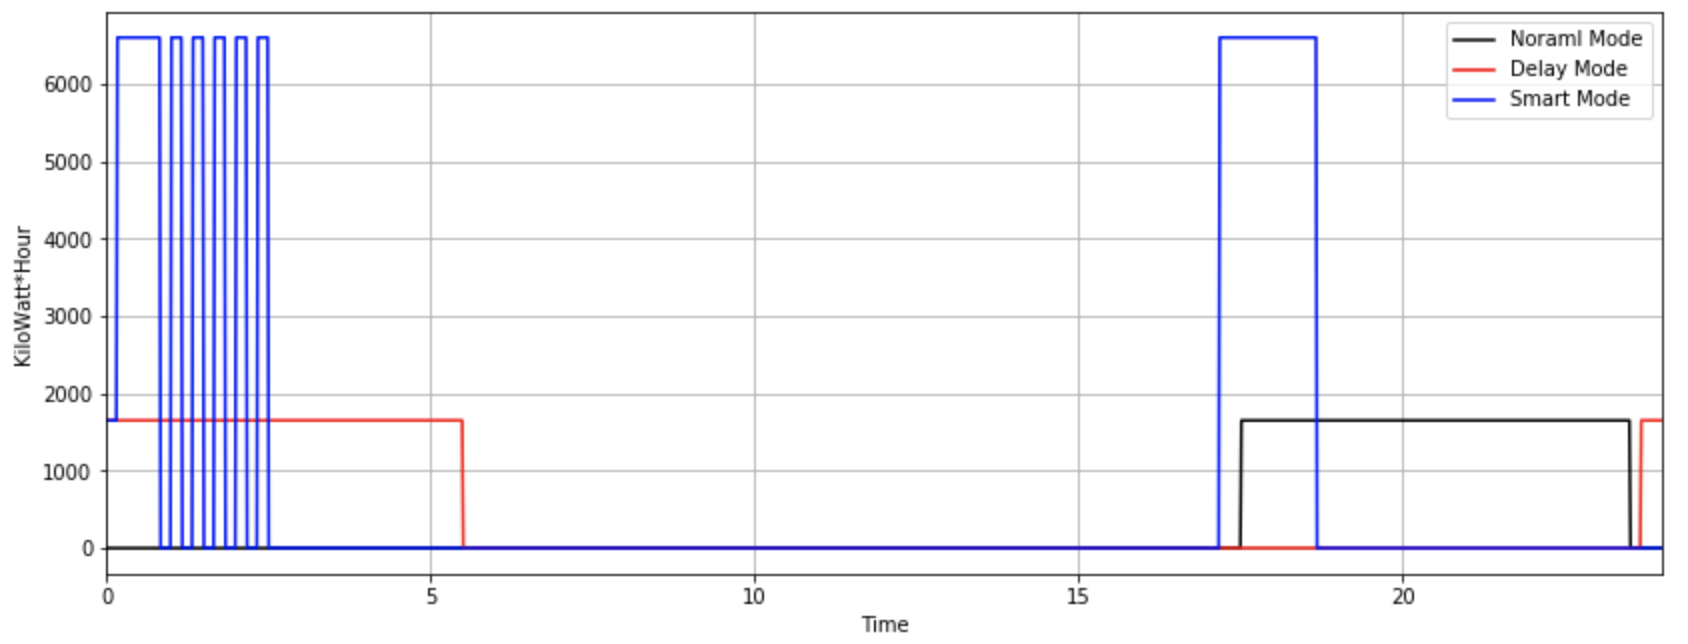
\includegraphics[scale=0.23]{simu_three_mode}}
                    \caption{Simulation results of three charging strategies}
                    \label{fig_simu_three_mode}
                \end{figure}

                An illustration of the three strategies is depicted in \hyperref[fig_simu_three_mode]{Figure \ref*{fig_simu_three_mode}}, where the real-time consumption of three strategies are separated obviously: the normal strategy has a continuous distribution starting from about 18:00, the delay strategy has a continuous distribution located at around 24:00, and the smart strategy results in a non-deterministic consumption as it is based on current state of the grid.
                \subsection{Simulating wind power generation}
                As it has been discussed that the wind power generation is directly related to the wind speed, and two linear regression models have been established in \hyperref[text_wind_regression_model]{Section \ref*{text_wind_regression_model}} to predict the power generation based on wind speed. Therefore, the concentration is attached on building a model for the wind speed. The statistics of wind speed has been analyzed in \hyperref[text_wind_speed_analysis]{Section \ref*{text_wind_speed_analysis}}. 
                
                It is the easiest idea to use a normal distribution, which is feeded by the analyzed mean and variance. The generated wind speed must be the same to the assumed statistics. However, the data should be located on the time series, which means that each generated random sample should be related to the previous ones. Assume all the wind speed of the whole day is $a_{day} = a_1a_2a_3\dots a_n$, where each $a_x$ is a random variable following the same normal distribution. From the \emph{Weak Law of Large Numbers} \footnote{In probability theory, the Law of large numbers states that the sample average of the sequences of i.i.d rvs: $A_{Y}^n = \frac{Y_1 + Y_2 + \dots + Y_n}{n}$ has the mean: $\mu_A = \mu_Y$, and the variance: $sigma_A^2 = \frac{\sigma_Y^2}{n}$.}, it is these i.i.d rvs make $a_n$ the same distribution as the sampled data. If the samples are related to the previous outputs, this generation should be a \emph{Markov Chain}, which models dependent rvs best. For \emph{Markov Chain}, the states and the transition matrix should be predefined to reflect the distribution of wind speeds. Therefore, the problem actually changes to the determination of the transition matrix. If the whole project is to find a better model of simulation wind speed, this should be a good question. However, there is neither enough content, nor time to discuss this problem in this project.

                The implementation of a normal distribution cannot be used because the generated data should be continuous. The Markov model is neither able to be implemented in a short term. One compromised solution in this project is to select the wind data in real world. To let the data fully reflects all the scenarios of wind speed, various days should be chosen carefully. 
                Finally, there are 5 days selected in this project. \hyperref[fig_1202]{Figure \ref*{fig_1202}} depicts a typical increasing tendency, it has an average wind speed of 5 m/s. \hyperref[fig_1203]{Figure \ref*{fig_1203}} is a typical decreasing tendency, it has an average wind speed of 7.5 m/s. \hyperref[fig_1204]{Figure \ref*{fig_1204}} is a day with high wind speed all day, the average wind speed is 7.6 m/s. \hyperref[fig_1130]{Figure \ref*{fig_1130}} is a day with low wind speed all the time, the average wind speed is 2.3 m/s. The last one is in \hyperref[fig_1107]{Figure \ref*{fig_1107}}, which has an average of 5.7 m/s and is close to the mean from the global view. It is assumed that these five scenarios can reflect all weather conditions, and thus support reasonable analysis.

                The actual implementation of the weather condition is based on an nonuniform random distribution. The reason is that the first four selected cases have the means not near the global the mean, and the 5th weather condition should be the normal one. The problem can be expressed as: $ 5.0 a_1 + 7.5 a_2 + 7.6 a_3 + 2.3 a_4 + 5.7 a_5 = 6.01 $, where $a_1 a_2 \dots a_5 $ are the coefficients of the probability function of random variable $X$ as the weather condition.
                A solution used in the simulation system is indicated in \hyperref[table_pf_coeff]{Table \ref*{table_pf_coeff}}.
                
                \begin{table}[ht]
                    \centering
                    \begin{tabulary}{\linewidth}{c c c c c}
                        \hline
                        $a_1$ & $a_2$ & $a_3$ & $a_4$ & $a_5$ \\ \hline
                        0.12 & 0.23 & 0.08 & 0.12 & 0.45 \\
                        \hline
                    \end{tabulary}
                    \caption{The implementation of the 5 coefficients of the p.f.}
                    \label{table_pf_coeff}
                \end{table}

                It can be found that the 5th weather condition has the most significant weight. The reason is the it is the most common weather. The weight of the extreme weather, the 3rd and the 4th conditions, have a sum of 0.2. The synthesized mean of this implementation is 5.8. Now the wind speed simulation satisfies both the requirements on the statistical characteristics and the real world nature of wind.

                \begin{figure}[ht]
                    \centerline{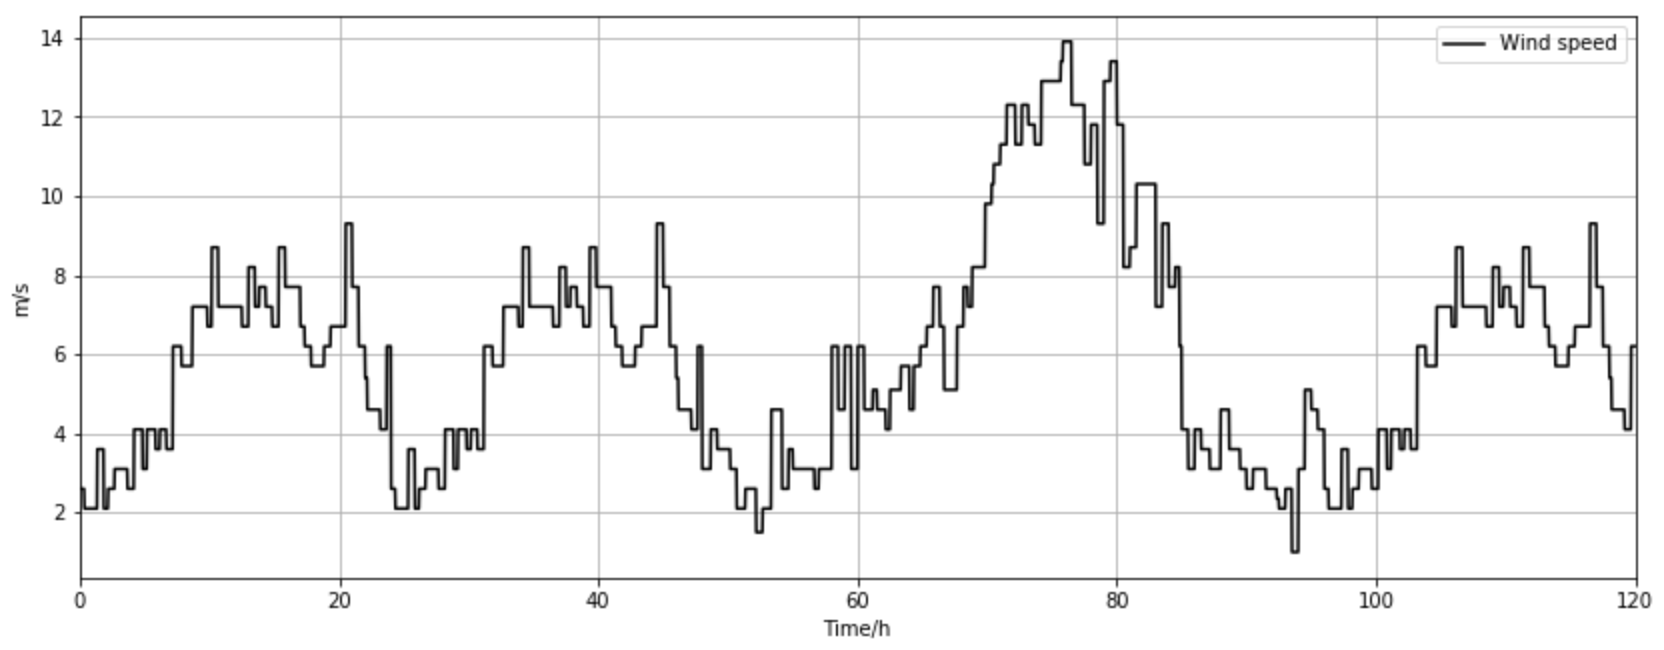
\includegraphics[scale=1]{simu_wind_speed}}
                    \caption{An illustration of the results of wind speed during a 5-day-interval (5*24=140h)}
                    \label{fig_simu_wind_speed}
                \end{figure}

                \hyperref[fig_simu_wind_speed]{Figure \ref*{fig_simu_wind_speed}} shows one result of the simulation system with a 5-day-interval. Though 5 days are simulated, three weather conditions are happened, as the 5th weather condition has a larger weight. The average wind speed of these five days is 5.9 m/s, and the standard deviation is 2.76 compared to that of data set at 3.42. This result is accepted.

                \subsection{Simulating grid storage}
                The storage is simply a battery, which is recharged when the demand is lower than the generation, and is discharged when the generation cannot satisfy current demand. When SoC is empty and the demand is higher than the generation, the imported energy is used. When SoC is full and the generation is higher than the demand, the curtailment is set to cut down some wind turbines and export energy.

            \section{Determining the storage}
            The implementation of the simulation has been elaborated, while two important parameters have not been determined: the scale factor of the wind farm and the storage of the grid. 

            \subsection{Determining the scale of the wind farm}
            Because it is a small grid with only 10 to 20 households, the scale of the wind farm should be at an appropriate range to reflect the condition in Orkney. If the scale is too low, the generation will fail to satisfy the demand most of the time. If the scale is too high, there is no need to use storage to compensate the shortcut. A practical understanding of the generation to the demand is extracted from the collected data set that by measuring the $Generation to Demand (G2D) = Generation\, Power - Demand\, Power $, 39\% of the time, the generation cannot satisfy the demand. From the perspective of the overall generation to overall demand, the average generation is $22.52 MWh$ from \hyperref[table_statistical_characteristics_generation]{Table \ref*{table_statistical_characteristics_generation}}, and the average of demand is $19.04 MWh$ from \hyperref[table_demands_properties]{Table \ref*{table_demands_properties}}. Thus, the simulated total generation to demand value should be positive and the line in the figure should have many downward parts to indicate the 39\% unsatisfied time.

            To determine the scale factor, a metric based on assumed performance is established. The overall generation to demand on the plot is used. The line of the appropriate scale should often above $ y = 0$ to satisfy the feature of average, and the line should many downward parts to satisfy the statistics of generation to demand. \emph{Monte Carlo simulation} is used to find the optimized scale factor. The time interval is 4 days, as there are four typical weathers in this simulation, and the scale factor is tested from 50 to 1100.

            \begin{figure}[ht]
                \centerline{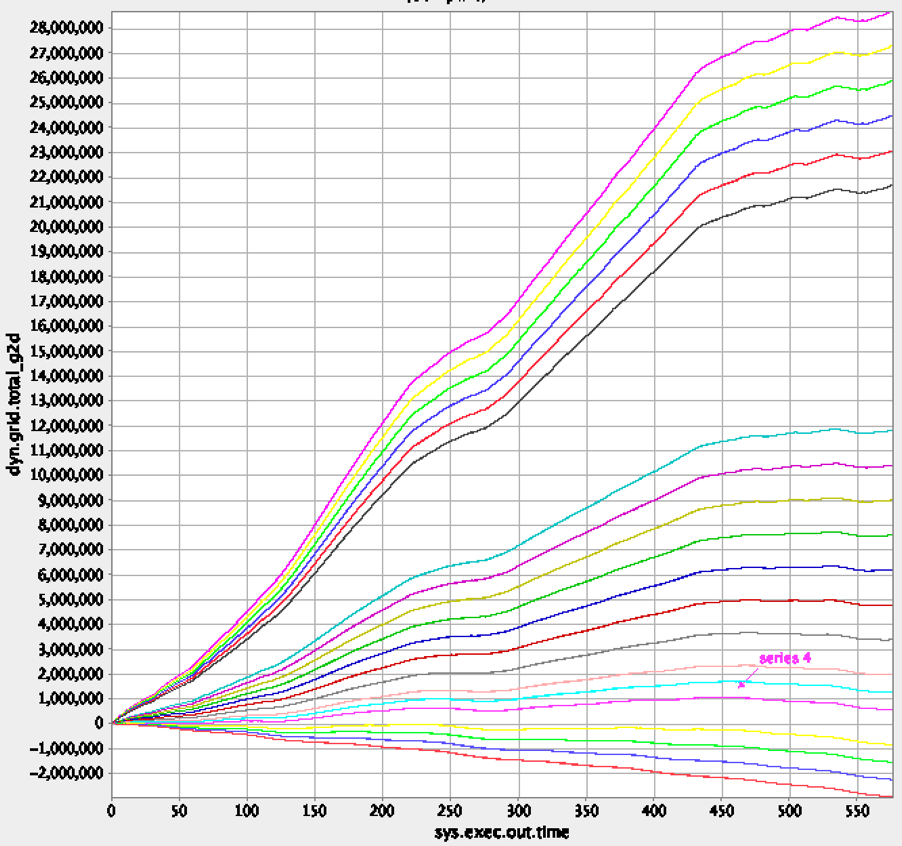
\includegraphics[scale=1.7]{scale_factor}}
                \caption{The plot of the simulated total generation to demand under various scale factors. (Generated by \emph{trick-dp})}
                \label{fig_scale_factor_monte}
            \end{figure}

            \hyperref[fig_scale_factor_monte]{Figure \ref*{fig_scale_factor_monte}} shows the results of testing different scale factors. Apparently, the fifth and sixth lines are the scale factors that mostly satisfy the requirements of the model. The value is 300 on the \emph{series 4} arrow, and this value is selected as the scale of the wind farm. On the other hand, this value should estimate the lower bound of the wind farm, as there are more wind turbines added later.

            \subsection{Determining the storage}
            \label{text_determine_storage}
            The determination of storage is based on all previous work, as only until the demand and generation have been simulated, will it is possible to estimate the storage of the grid. A proper storage can not always be empty, as it should provide energy to compensate the unstable feature of wind generation, nor this storage be always full, as the curtailment will happen frequently, causing more waste on potential generation. 
            
            Therefore, a metric is defined to estimate the quality of the current storage: the portion of time the SoC of the grid storage is in the range 15\% to 80\%. 
            \begin{equation}
                Quality\, Of\, Storage = \frac{Total \, time\, of \, (15\% \leq SoC \leq 80\%)}{Total \, time}
            \end{equation}

            It is the percentage of health condition, and it is quantified as a score between 0 and 1. From the definition provided, the closer it is approaching to 1, the better the storage is satisfying the requirements.

            However, this single numeric value also has some limitations. Assume the storage is so large that any power generation or demand in the grid cannot attach any apparent change to the SoC. If the initialized SoC is at 90\%, the score will be nearly 0. A similar result can be acquired from a initial SoC at 10\%. The storage of the battery definitely satisfies the requirement, but the metric fails to detect it \footnote{Although the two assumed initial SoCs result in the battery always in a condition not beneficial to the battery life, the large storage makes it possible to accommodate the need to store enough energy to compensate for the less windy days.}.

            On the other hand, the task is to find a storage that appropriately satisfies the need. That is to say, too large storage introduces waste as most of the storage will not be efficiently used, too small storage is not adequate for providing energy in peak hours.

            To have more information on how the current storage of battery behaves, the average SoC and the portion of time that the SoC is at 0 are also estimated.

            Then, the initialize SoC of the grid storage should be determined. Two kinds of initialization are considered: the initial SoC is at a constant value for all value of capacities, and the initialize SoC is at a constant percent of the capacity. The reason why these two initializations differ is that if the constant SoC is chosen, the constant can be too small for larger capacities so that it will possibly be out of the health range at the beginning, and it will take longer time to reach the health range with the scale of the wind farm not changed. The initial state definitely affects the score, and this is what should be avoided. A compromising method is to set initial SoC to 0 for all tests, then the constant and percent initial states are both satisfied.

            Additionally, a longer simulation interval is also necessary to minimize the effects of initial SoC. Theoretically, as the simulation introduces randomness, the longer the simulation period is, the more the results adhere to the predefined statistical characteristics \footnote{This can be elaborated by \emph{Weak Law of Large Numbers} \cite{paper:wlln}.}.

            The length of simulation is set to 30 days. The number of houses is 20. And there are no EVs in the grid. It is necessary to first find an appropriate storage for the grid without penetration of EVs, then the impact can be quantized by discrepancies of scores.

            A new problem is that range of the test data should be determined first. \hyperref[fig_extreme_case]{Figure \ref*{fig_extreme_case}} in the Appendices shows an extreme case, where there is no higher wind speed all day long that the generation cannot support the demand. If the battery is to assume this case as the worst case, it should be able to support the demand for the whole day without outer generation. From simulation, this value for 20 houses is 152728 kW h. In practical cases, there must be some generation from the wind farm, thus, the storage should be smaller than this value. The simulation tests the range of storage from 15,000 kW h to 100,000 kW h.

            \begin{figure}[ht]
                \centerline{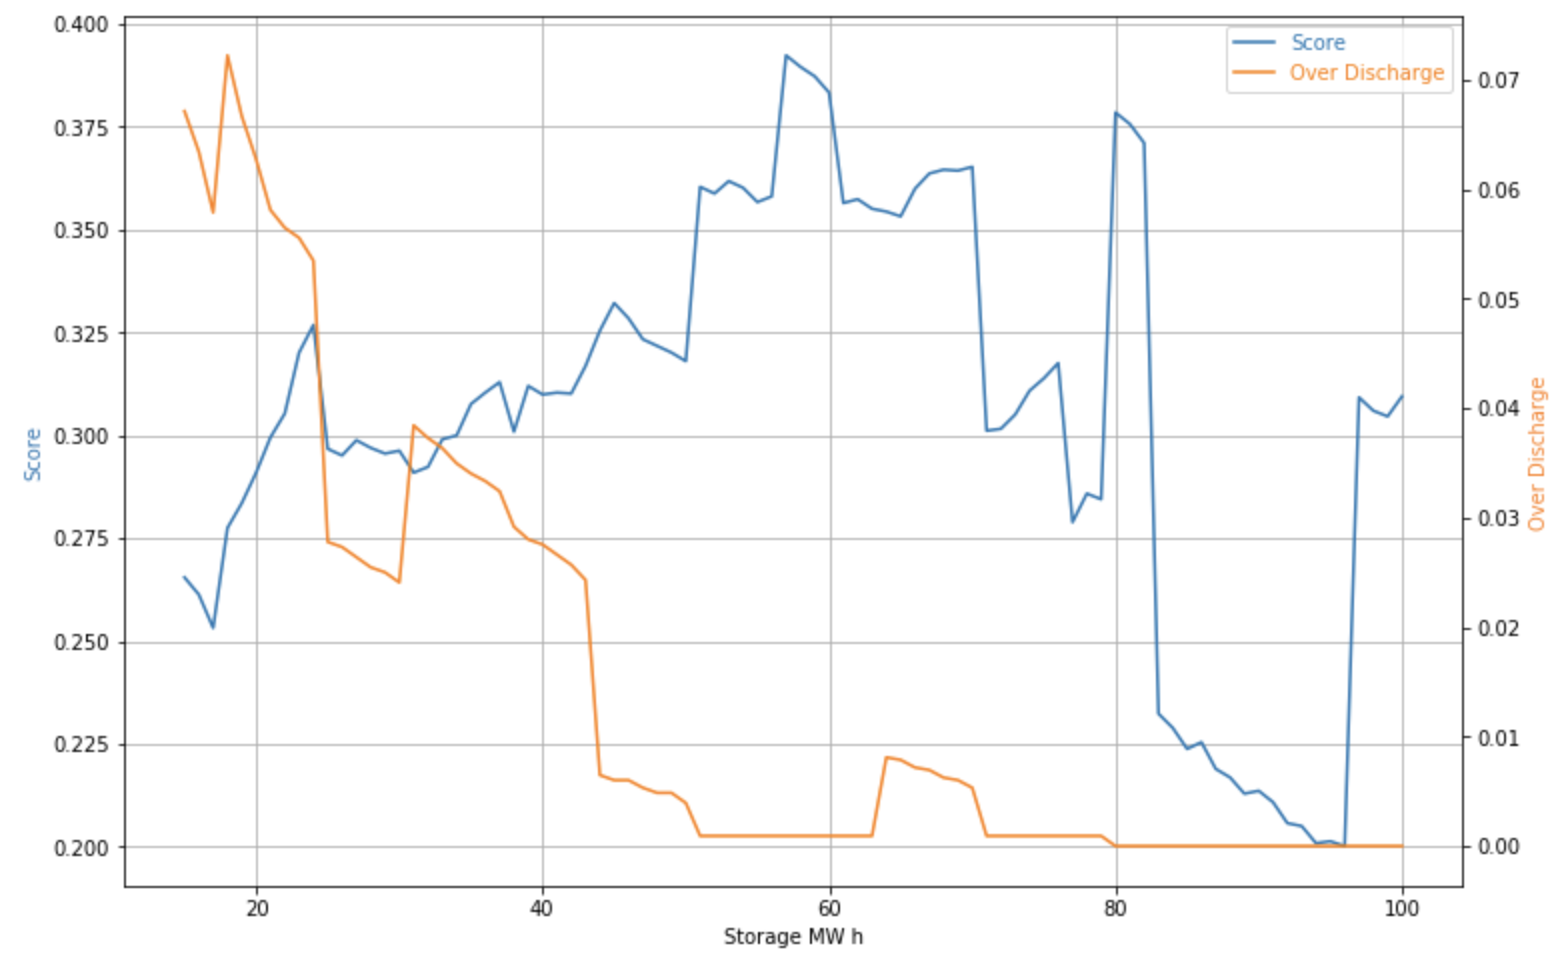
\includegraphics[scale=0.85]{simu_score}}
                \caption{The scores and over-discharges in the range of storage from 15 MW h to 100 MW h}
                \label{fig_simu_score}
            \end{figure}

            \hyperref[fig_simu_score]{Figure \ref*{fig_simu_score}} illustrates the results. It can be found the percent of over-discharge has a decreasing tendency with the increasing storage. It can be explained intuitively that larger storage is unlikely to be fully discharged. However, the score is not increasing with the storage grows. The highest score is at when the storage is 57 MW h, and the storage larger than 80 MW h perform badly. This can be explained by the average SoC \footnote{Remember that three metrics are recorded to fully evaluate the current storage: Quality factor, average SoC, percent of over-discharge.}, as the rate of over-discharge is decreasing, the grid storage can only be fully charged which cannot satisfy the range of health. 

            \begin{table}[ht]
                \centering
                \begin{tabulary}{\linewidth}{C C C C C}
                    \hline
                    Capacity (MW h) & 81 & 85 & 90 & 100 \\ \hline
                    Average SoC (MW h) & 65.7 (81\%) & 73.9 (87\%) & 78.7 (87\%) & 83.6 (83\%) \\ \hline
                    Score & 0.38 & 0.22 & 0.21 & 0.31 \\
                    \hline
                \end{tabulary}
                \caption{The average SoC of some high storage simulations}
                \label{table_high_storage}
            \end{table}

            \hyperref[table_high_storage]{Table \ref*{table_high_storage}} records the average SoC of some of the high storage simulation along with their ratio to the capacity. An average at over 80\% definitely introduces most of the time the battery being over charged.

            From the perspective of battery health, the storage does not have a good performance. On the other hand, it reflects the fact that the wind power generation has the potential to support the demand and provide more energy to be stored and exported. Though the high capacities have low score, but they are never over-discharged, this can make them much safer if the penetration of EV is increased.

            \section{Simulating the impacts of EV penetrations}
            The previous work makes it possible to quantize the impacts of EVs and the efficiency of charging strategies to fully use the wind power generation. The results in previous section indicate that the generation is often so large that the grid storage is fully charged. It is reasonable that the penetration of EVs will somehow make the score higher than before, as it increases the demand, however, introduces more chances to let the battery fully discharged.

            There are three charging strategies, and penetration from 0 to 100\%. It is exhausting to test every penetration level on each strategy, thus, 10\%, 20\%, and 40\% are selected, and the impacts are compared. To be more accurate, the length of simulations increased to 60 days.

             
            As the strategies have been implemented in previous sections. This section only shows the results. The results are plotted on the parasite figure by each penetration and each charging mode. Thus, there are 9 figures in all.

            \subsection{Impacts of normal charging strategy}
            The normal strategy is to charge the EV whenever it is connected to the grid. This section shows the performance of normal charging strategy.

            \begin{figure}[htp]
                \begin{center}
                  \subfigure[The performance of the storage under 10\% penetration]
                  {\label{fig_simu_score_normal_10}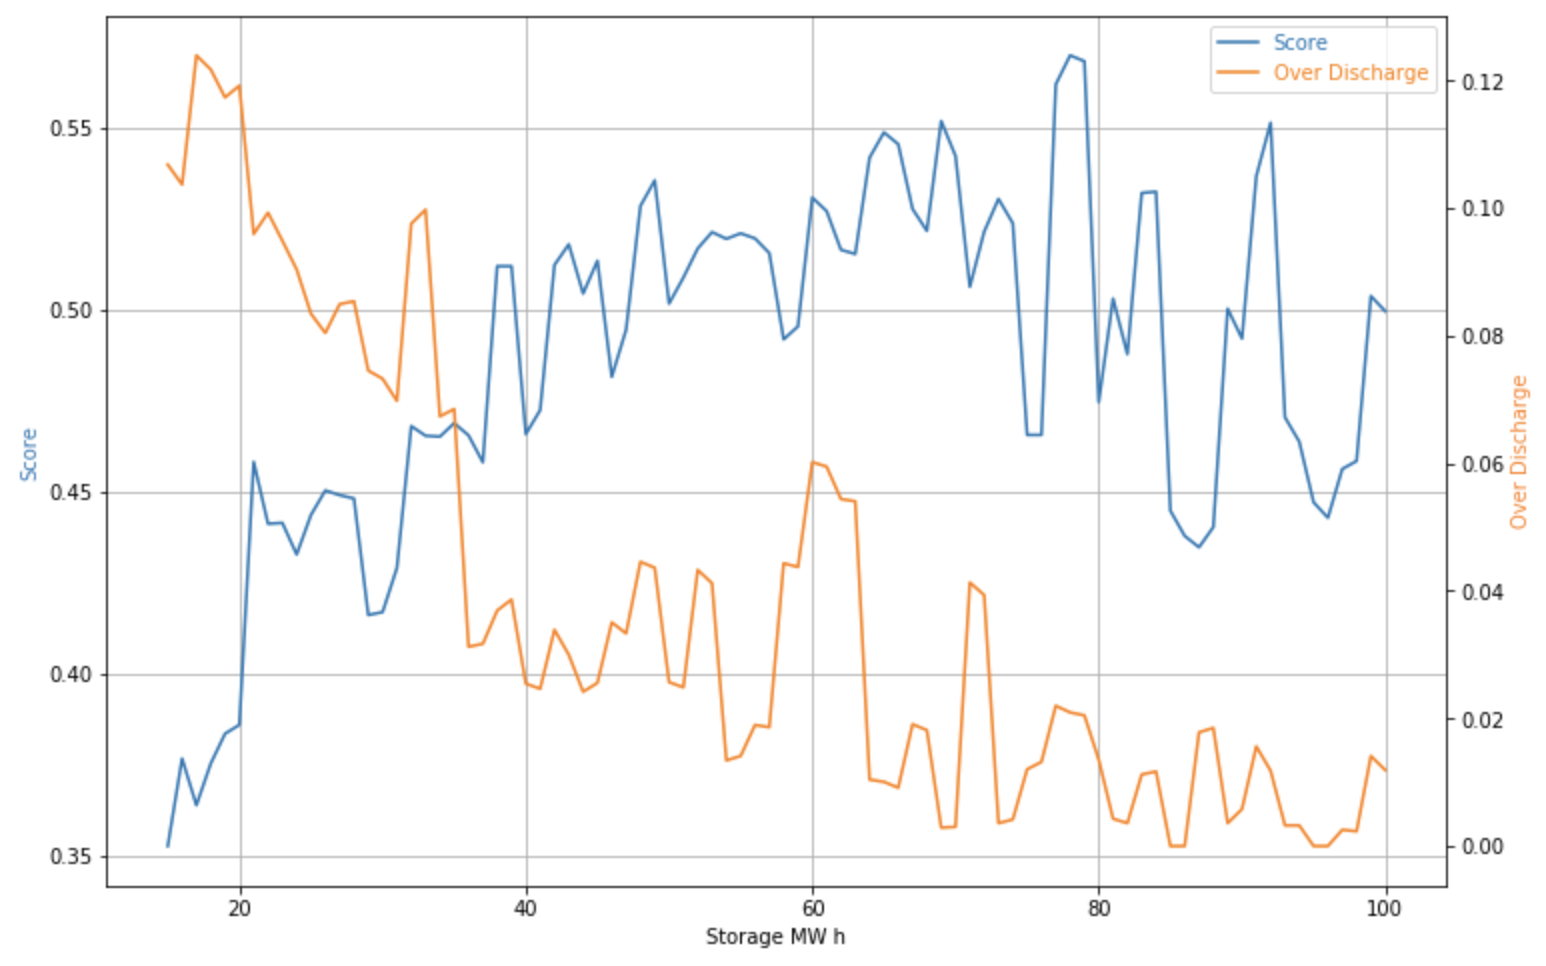
\includegraphics[width=.49\linewidth]{simu_score_normal_10}}
                  \subfigure[The performance of the storage under 20\% penetration]
                  {\label{fig_simu_score_normal_20}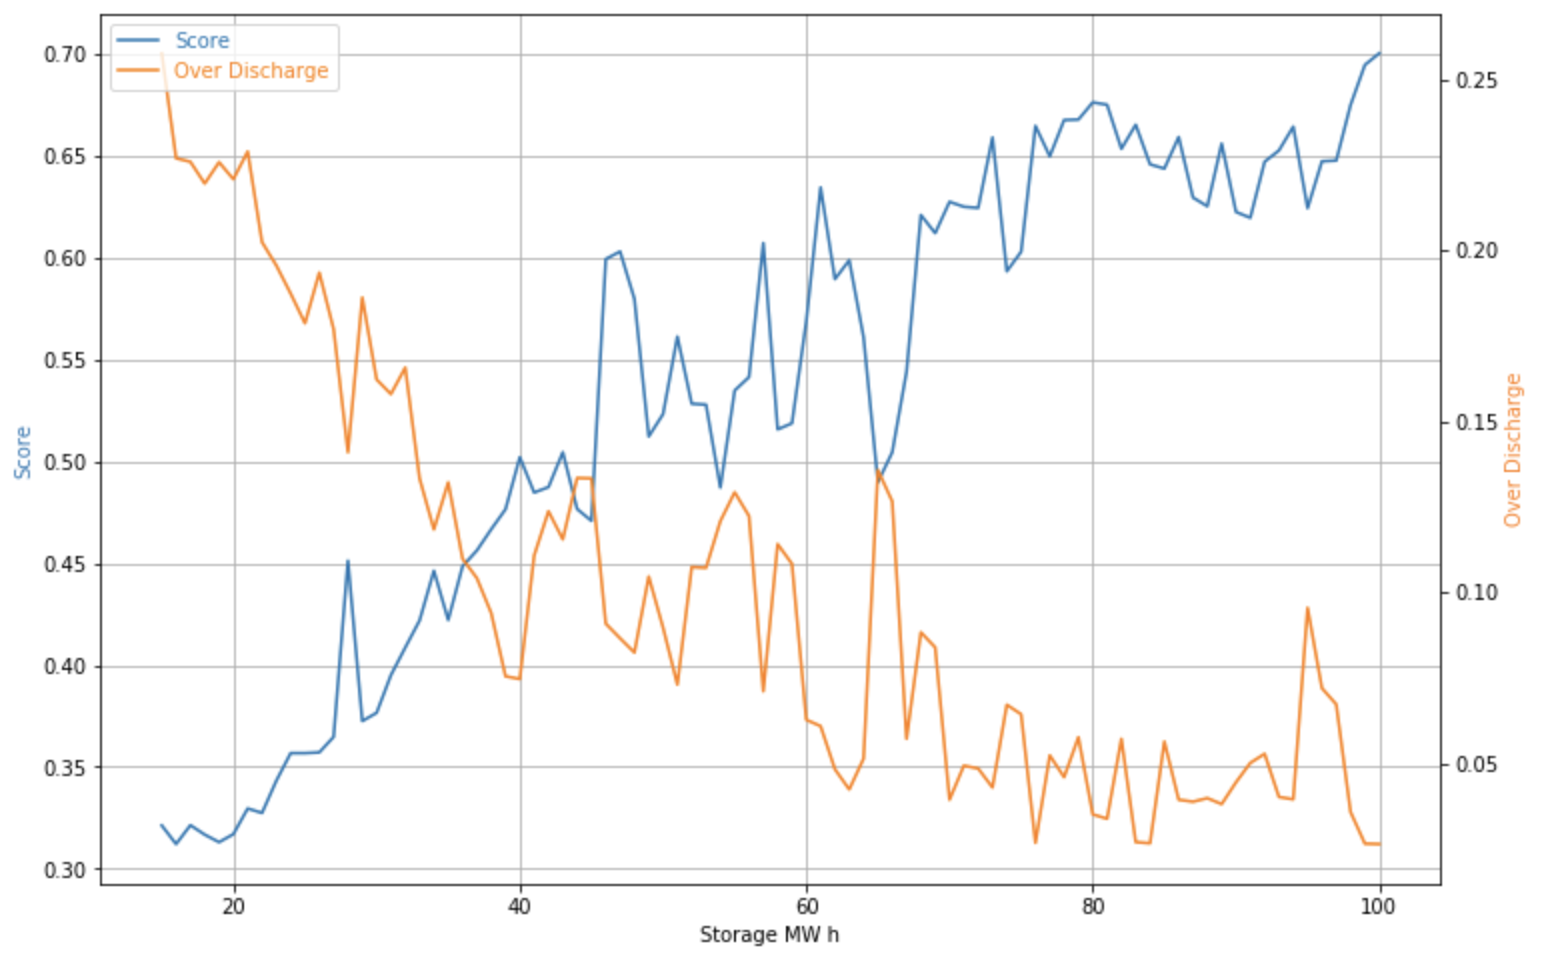
\includegraphics[width=.49\linewidth]{simu_score_normal_20}} \\
                  \subfigure[The performance of the storage under 40\% penetration]
                  {\label{fig_simu_score_normal_40}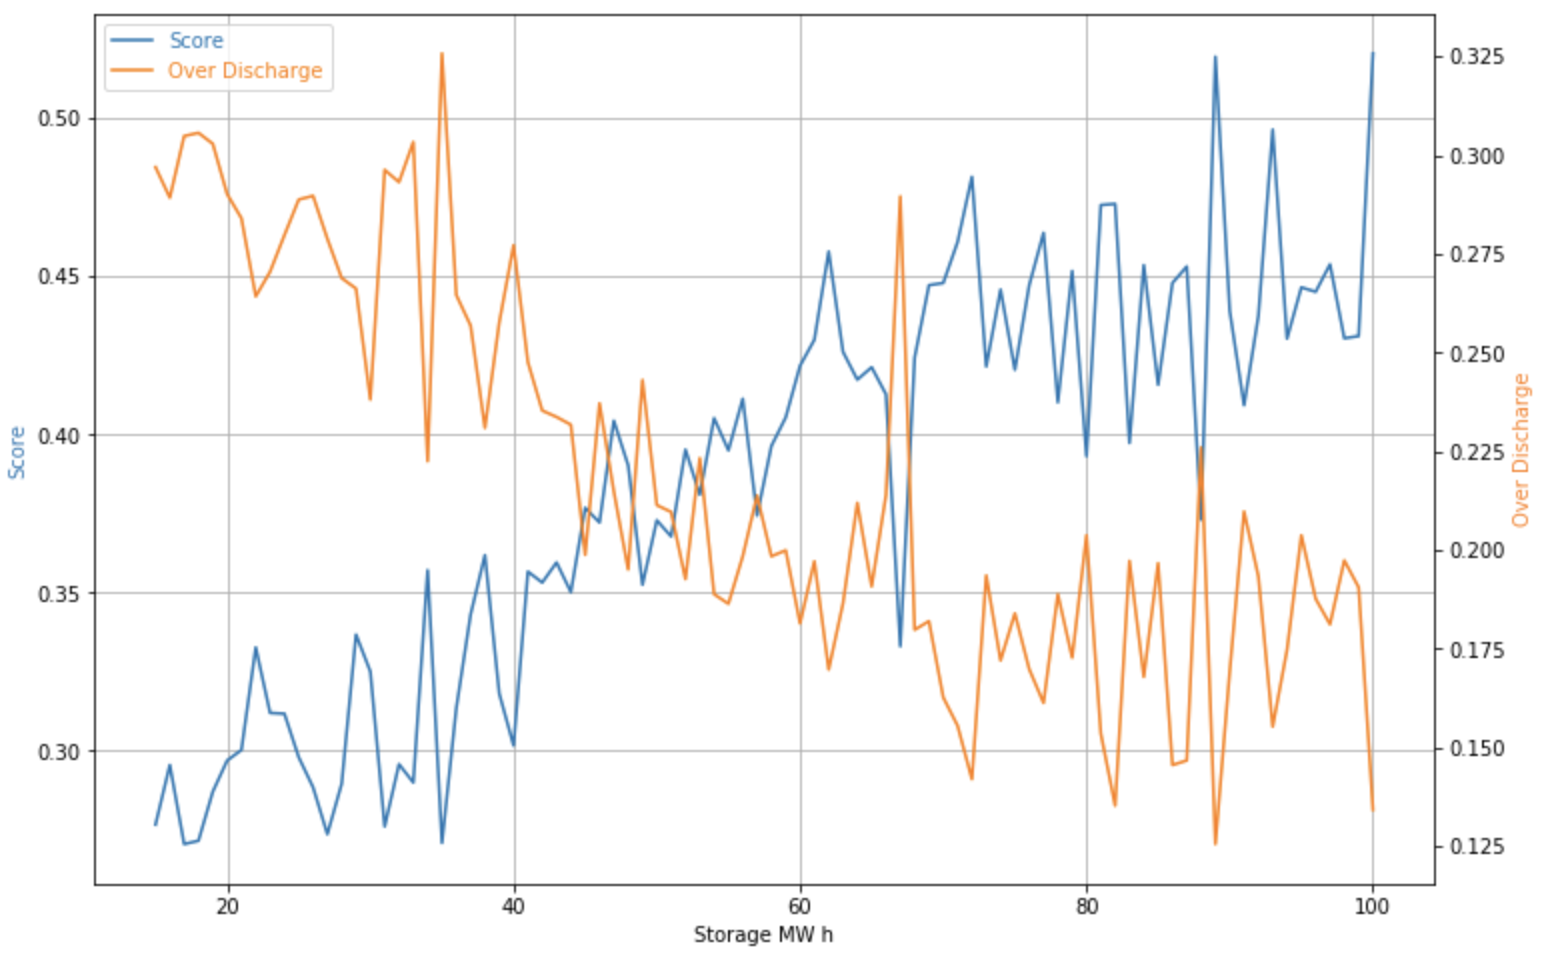
\includegraphics[width=.5\linewidth]{simu_score_normal_40}}
                \end{center}
                \caption{The performance of the storage under the normal charging strategy}
                \label{fig_normal_charging}
            \end{figure}
            
            \begin{table}[ht]
                \centering
                \begin{tabulary}{\linewidth}{C C C C C}
                    \hline
                    Capacity (MW h) & 81 & 85 & 90 & 100 \\ \hline
                    Average SoC (MW h) & 25.9 (31\%) & 21.4 (25\%) & 22.2 (25\%) & 25.6 (25\%) \\ \hline
                    Score & 0.47 & 0.42 & 0.44 & 0.52 \\
                    \hline
                \end{tabulary}
                \caption{The average SoC of some high storage simulations under 40\% penetration}
                \label{table_high_storage_40}
            \end{table}

            \newpage
            \subsection{Impacts of delay charging strategy}
            This section shows the results of delay charging strategy based on the same simulation schema in testing normal charging strategy.

            \begin{figure}[htp]
                \begin{center}
                  \subfigure[The performance of the storage under 10\% penetration]
                  {\label{fig_simu_score_delay_10}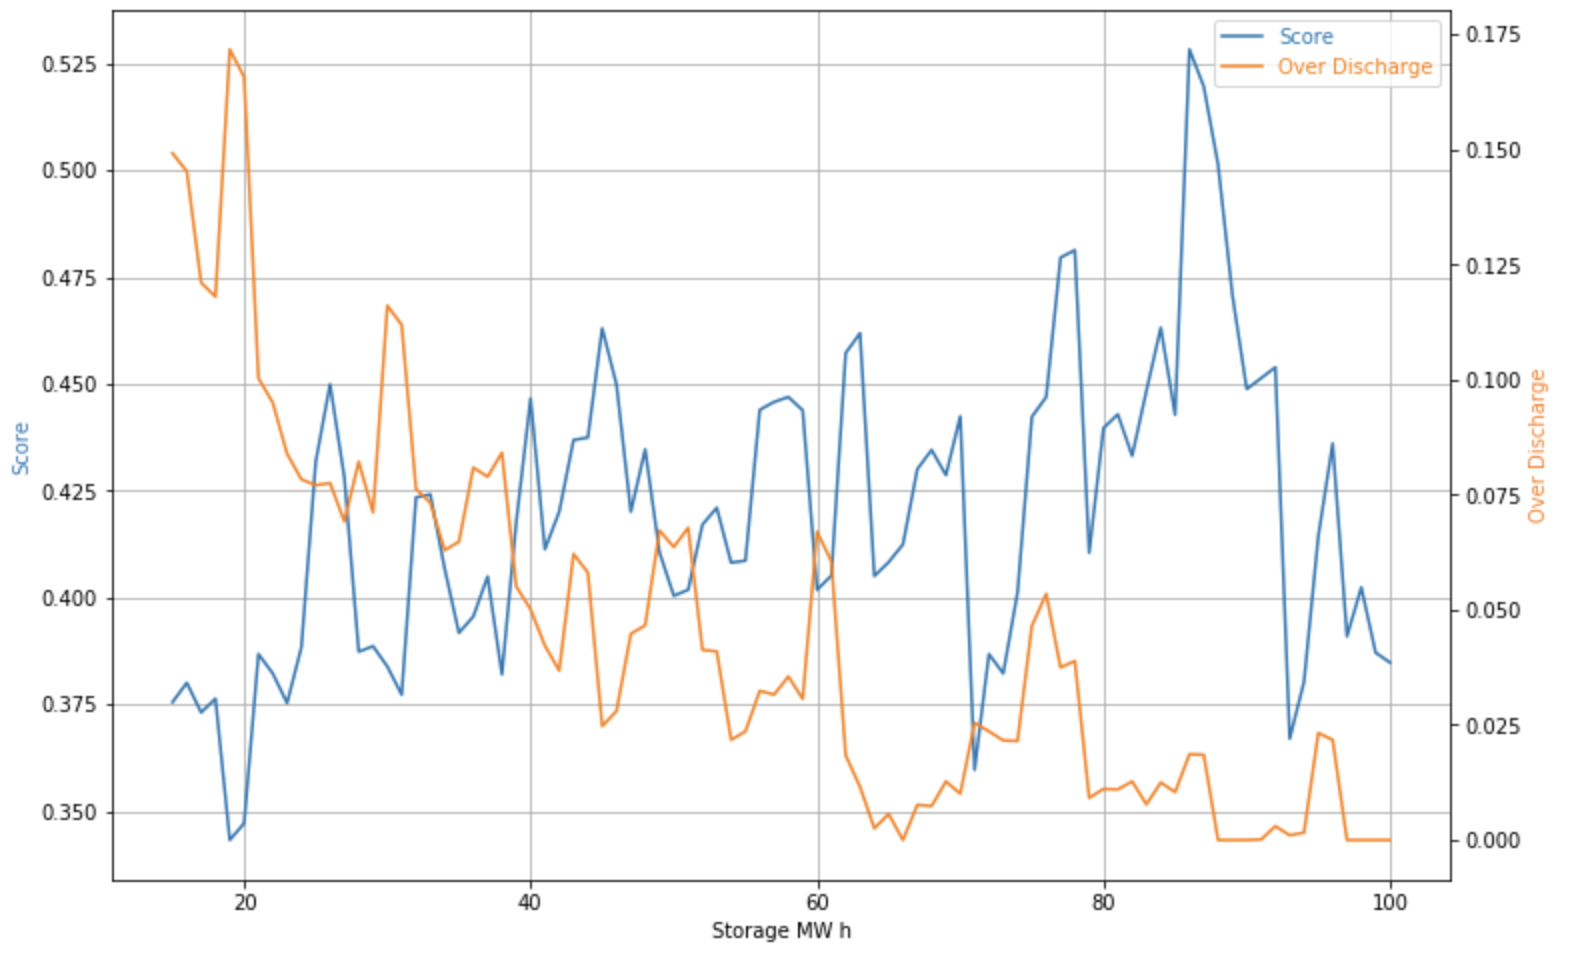
\includegraphics[width=.49\linewidth]{simu_score_delay_10}}
                  \subfigure[The performance of the storage under 20\% penetration]
                  {\label{fig_simu_score_delay_20}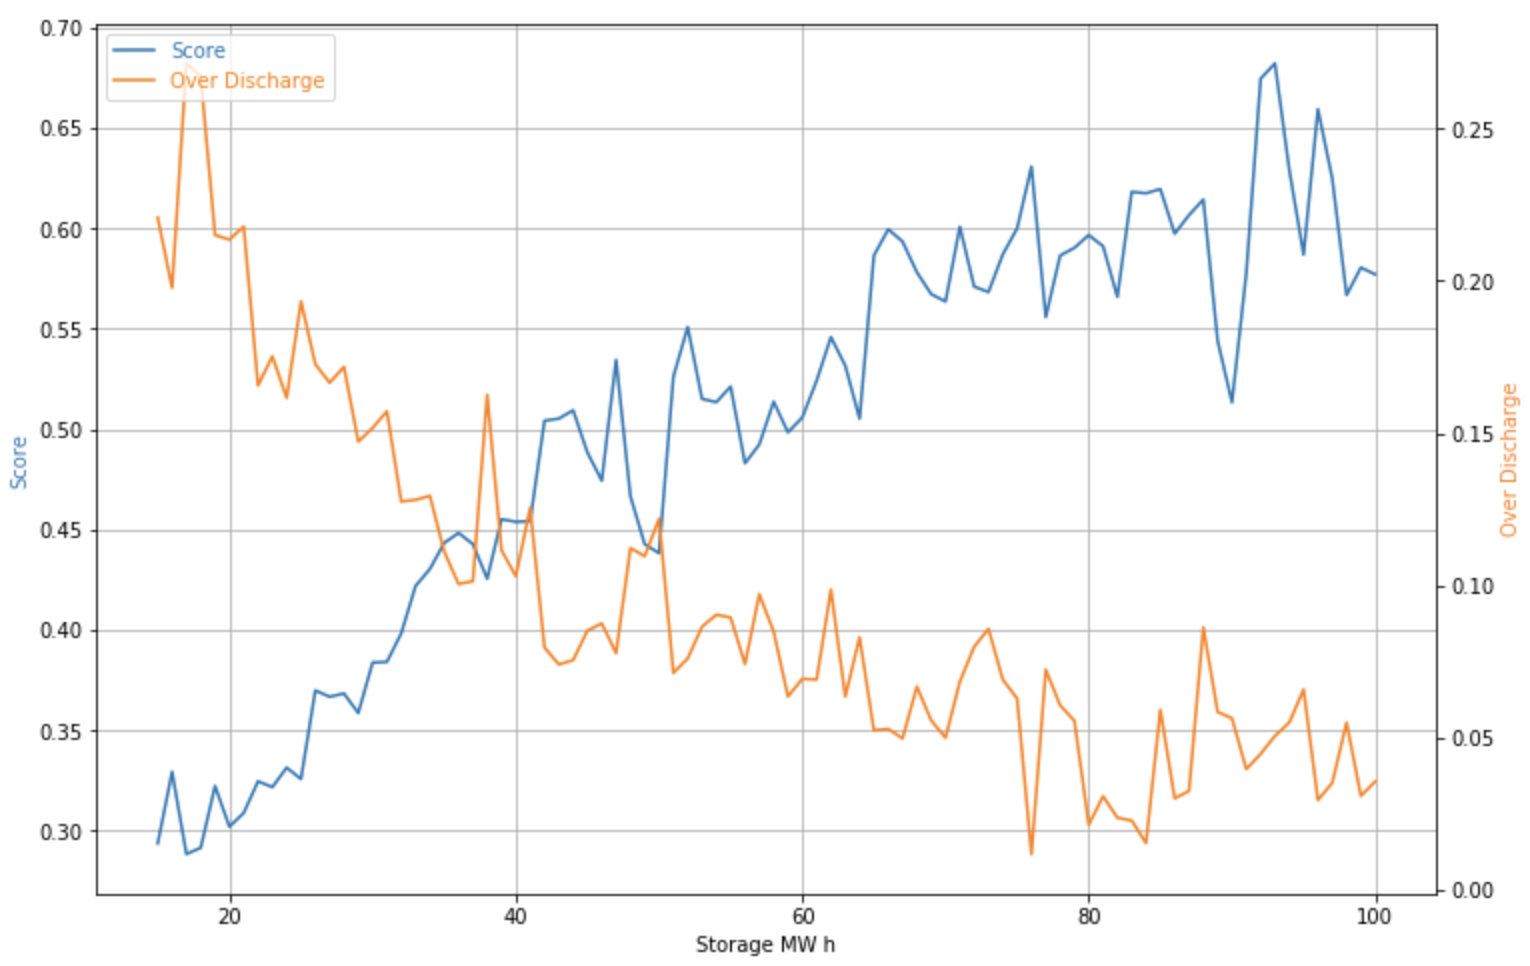
\includegraphics[width=.49\linewidth]{simu_score_delay_20}} \\
                  \subfigure[The performance of the storage under 40\% penetration]
                  {\label{fig_simu_score_delay_40}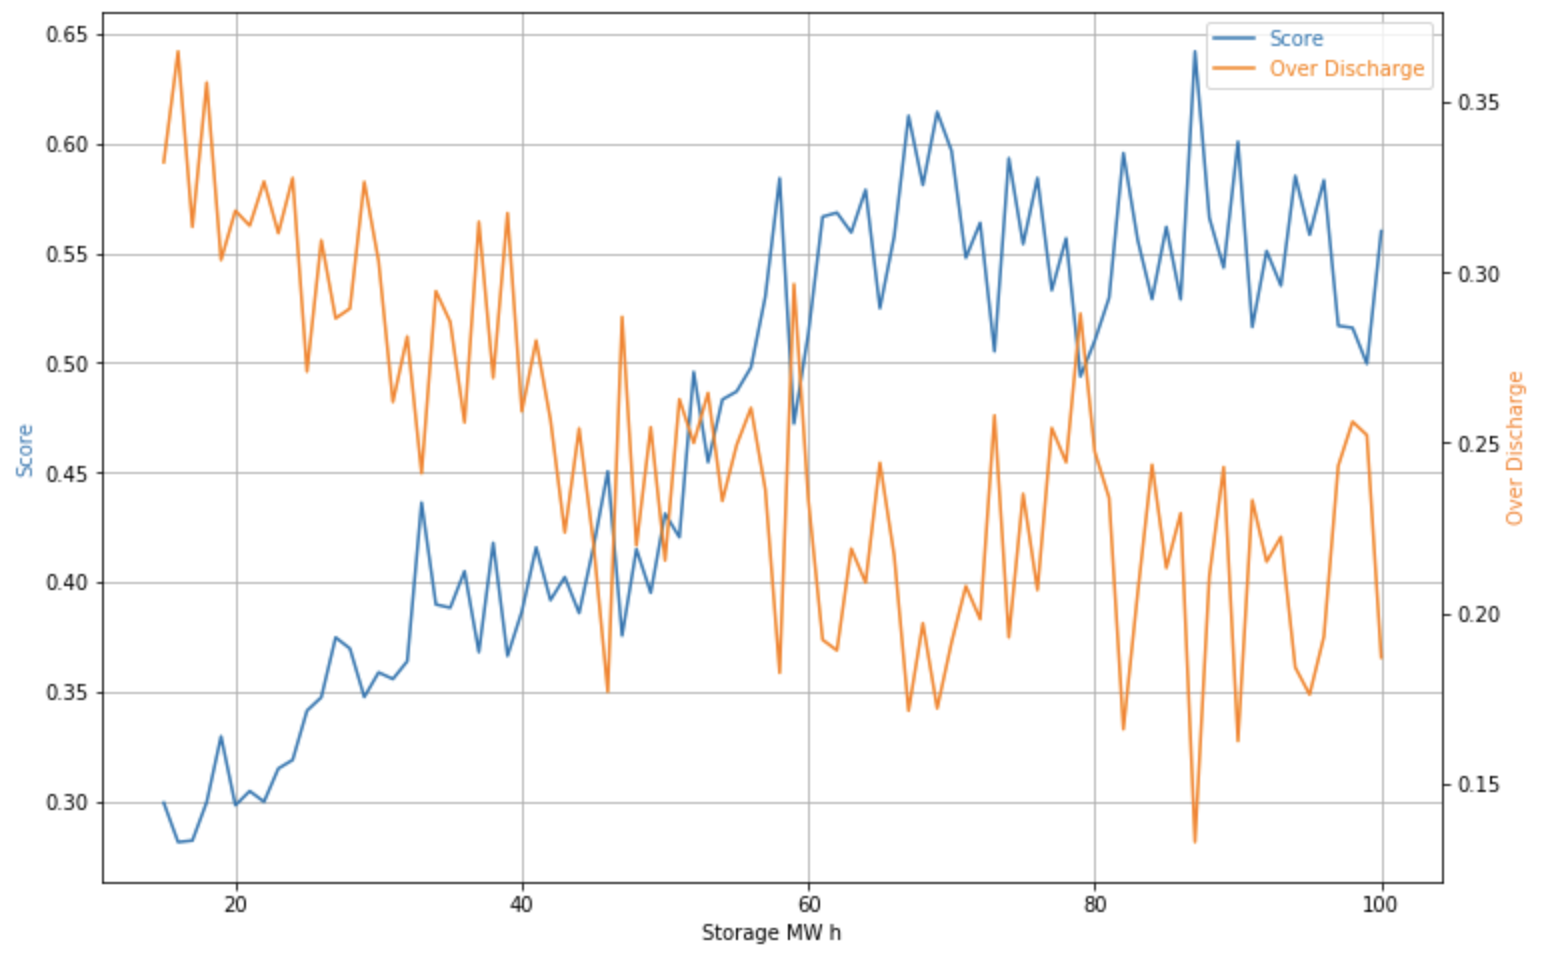
\includegraphics[width=.5\linewidth]{simu_score_delay_40}}
                \end{center}
                \caption{The performance of the storage under the delay charging strategy}
                \label{fig_delay_charging}
            \end{figure}
            
            \newpage
            \subsection{Impacts of smart charging strategy}
            This section shows the results of smart charging strategy based on the same simulation schema in testing normal charging strategy.

            \begin{figure}[htp]
                \begin{center}
                  \subfigure[The performance of the storage under 10\% penetration]
                  {\label{fig_simu_score_smart_10}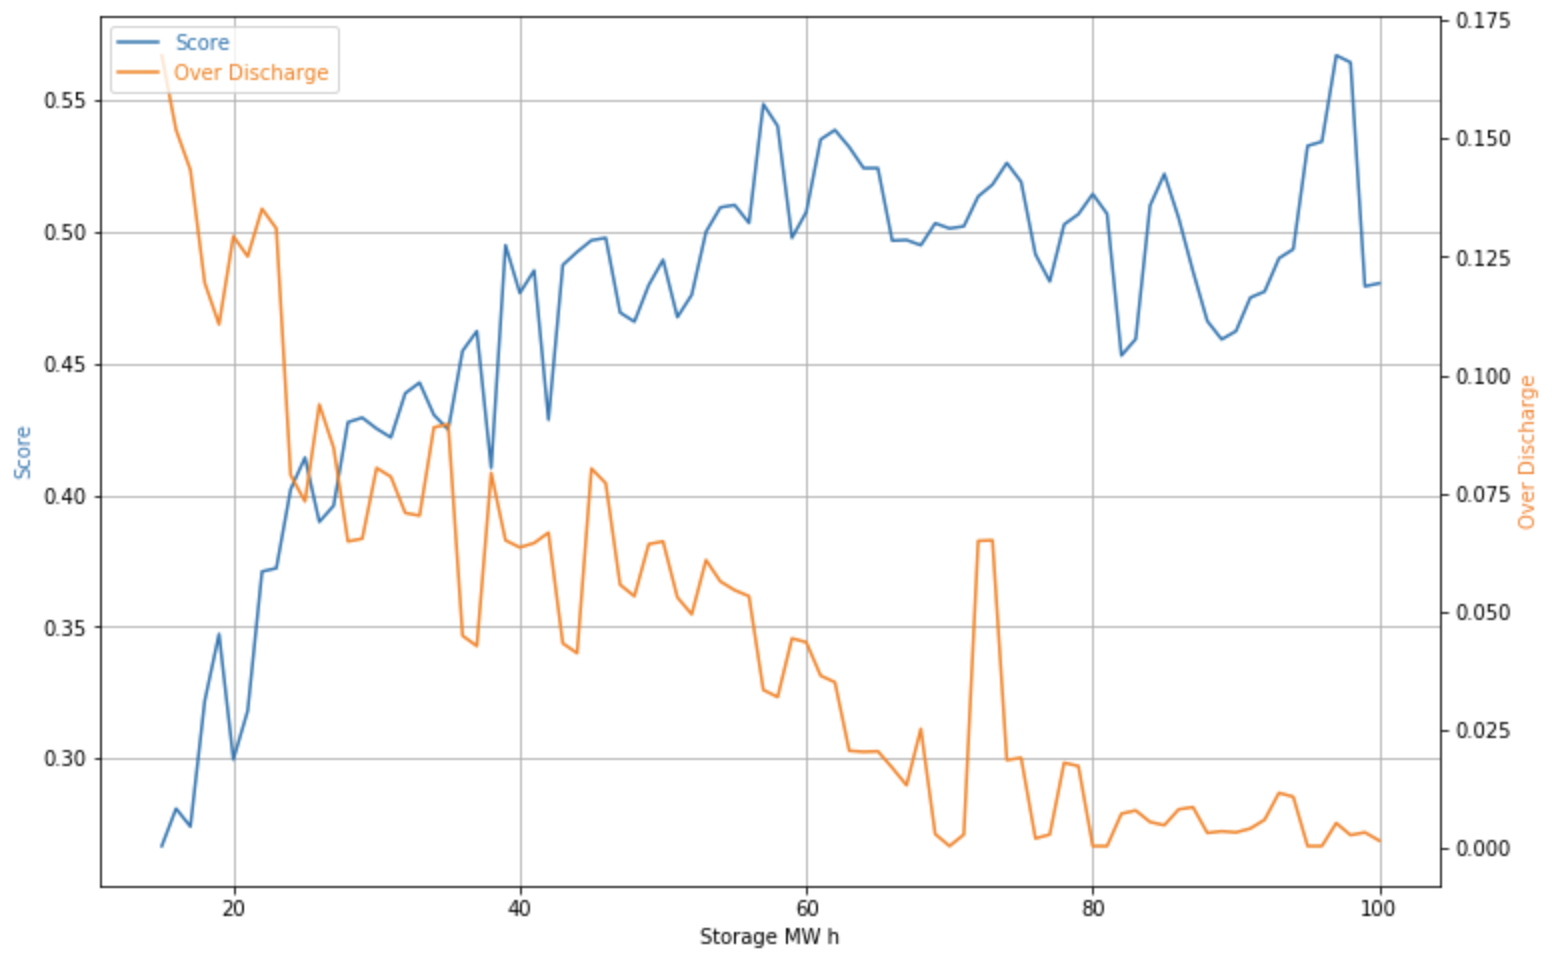
\includegraphics[width=.49\linewidth]{simu_score_smart_10}}
                  \subfigure[The performance of the storage under 20\% penetration]
                  {\label{fig_simu_score_smart_20}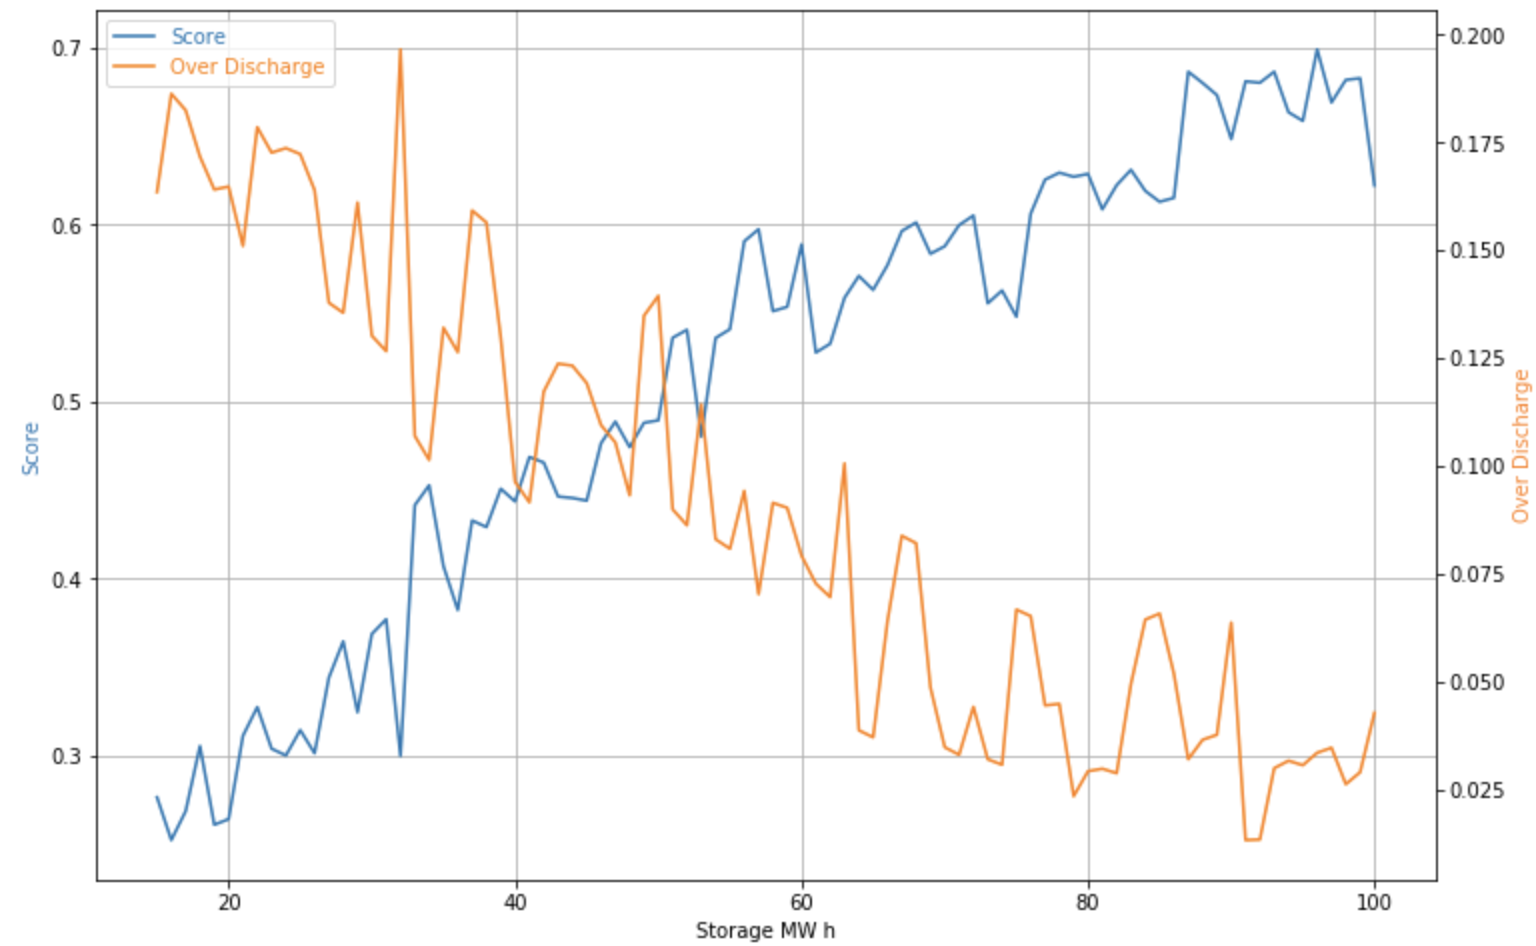
\includegraphics[width=.49\linewidth]{simu_score_smart_20}} \\
                  \subfigure[The performance of the storage under 40\% penetration]
                  {\label{fig_simu_score_smart_40}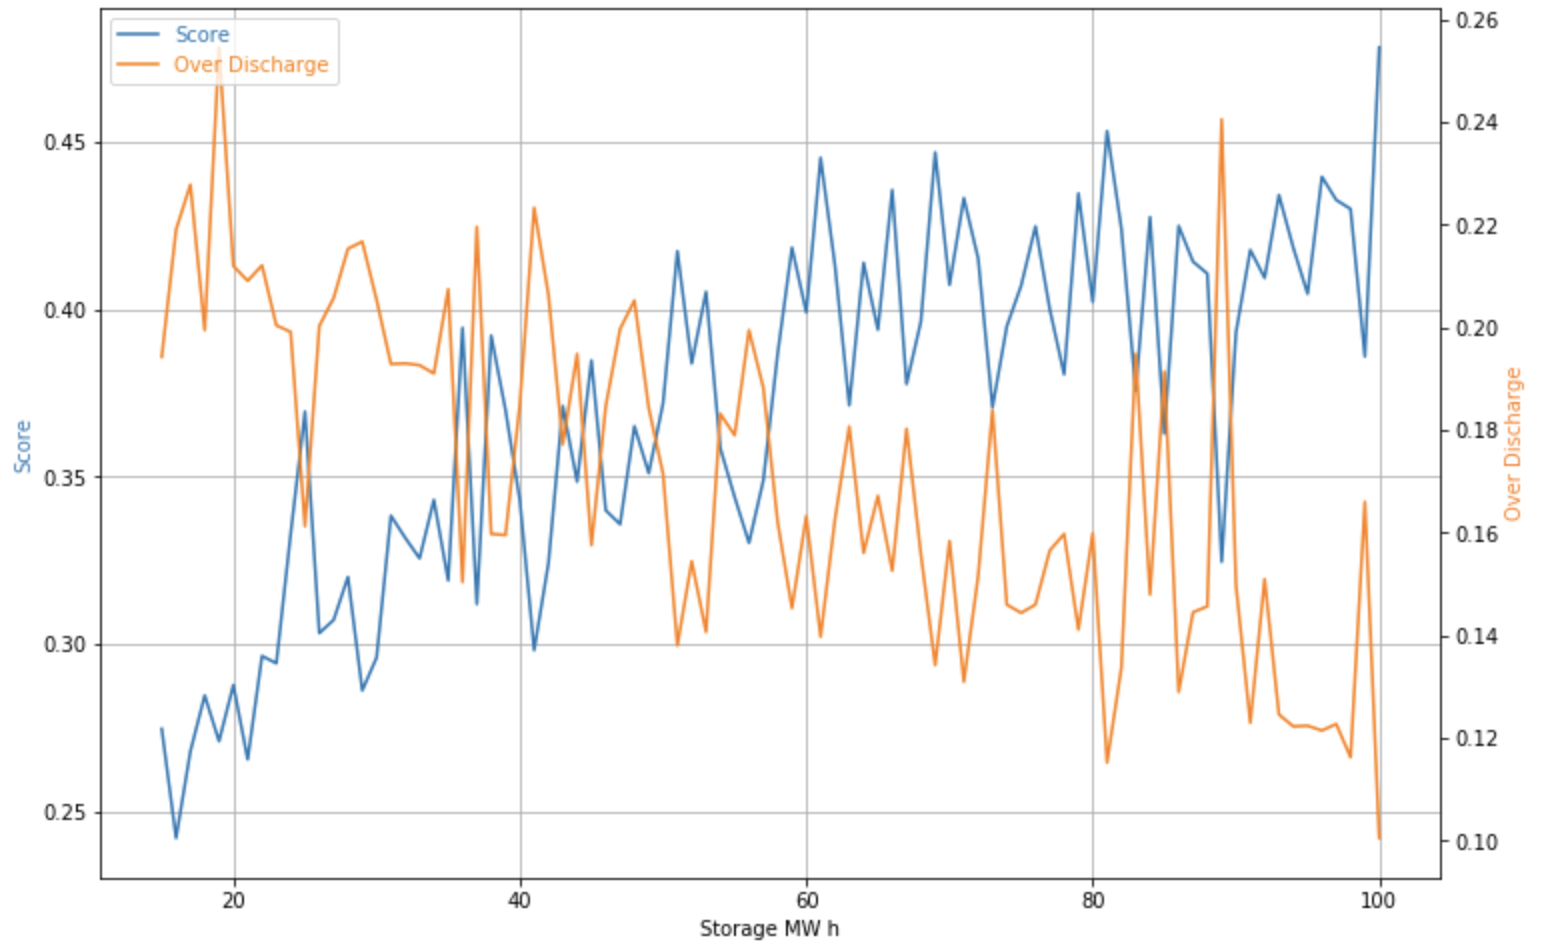
\includegraphics[width=.5\linewidth]{simu_score_smart_40}}
                \end{center}
                \caption{The performance of the storage under the smart charging strategy}
                \label{fig_smart_charging}
            \end{figure}

    \chapter{Conclusion}
    %The last chapter of your report must cover the conclusions. You discuss (briefly) the problems that arose which you had not anticipated, and how, as a result of this knowledge you would change the project. You discuss the projects limitations and discuss how these may be overcome. In short, you are clarifying the situation for the person who shall follow you and continue the project by pointing out where he needs to direct most of his efforts. As the project is only intended to create a prototype (except in certain special circumstances) there should be many useful modifications which you can suggest, and much from what you have experienced in your project work that you can impart to others. Consequently, of all the chapters in your report, the conclusions are probably the ones which best portrays your ability as an engineer.
    It is the non-determinism of both the wind and charging events of EVs that causes the instability of the grid. The extent of this non-determinism has been analyzed both by statistical methods and illustrating methods. 
        \section{Impact of wind}
        It has been explained in Introduction that the impacts of using wind as the resource of power generation introduces the need of storage to storage energy when generation is higher than demand, and the compensate the shortage when generation is lower than the demand. In Orkney, wind power generation can satisfy the demand 69\% of the time. The wind resource still has large potentials, as the curtailments, which indicate the wind speed is too strong, are frequently happening that it is reported that region A has over 20\% of the total time in a year under curtailment \cite{report:OrkneyAudit}.

        The simulation results in \hyperref[text_determine_storage]{Section \ref*{text_determine_storage}} also shows that the wind power can fully satisfy the daily demand if EV is not introduced. A capacity of 57 MW h, which is about $\frac{1}{3}$ of the total daily power demand, has the best performance in the grid.
        The grid storage is largely likely to be fully charged, though, the extra power can be exported or cut off. 
        
        When the EVs are added to the grid, over generated power can be absorbed and the score of the storage increases. The increasing trend meets the turning point before 40\% penetration level. This is the point that the wind farm generation can fully support. However, one limitation is that the wind power generation model is extracted from the Orkney data set, which has already introduced curtailment. If the curtailment level is alleviated to a higher value, the grid will be able to accommodate more EVs.

        \section{Impact of EVs}

        \hyperref[fig_simu_score_normal_10]{Figure \ref*{fig_simu_score_normal_10}} shows the score of normal under 10\% penetration. It can be found that most scores increases to 0.5, and the maximum score moves to higher capacity. The higher capacities behave better with lower over-discharge scores, while the performance is still not significant enough.
        For the score of delay strategy under this penetration in \hyperref[fig_simu_score_delay_10]{Figure \ref*{fig_simu_score_delay_10}}, the performance does not change too much. However, it is difficult to understand why the score on the map oscillates drastically. The pre-assumed results should be an increasing arc. A possible explanation is that the generation from the wind is still too large for the penetration of 10\%. In the end, the delay strategy does not result in progress on performance and the best score is also over 80 MW h.
        The smart strategy in \hyperref[fig_simu_score_smart_10]{Figure \ref*{fig_simu_score_smart_10}} shows an apparent tendency of performance progress, where the score grows significantly from 20 MW h to 40 MW h. It also shows that for storage larger thn 50 MW h, the performance converges to score 0.5. The advantage of this strategy is obvious, as the score is much more stable, and the rate of over-discharge is at an extremely low level.

        \hyperref[fig_simu_score_normal_20]{Figure \ref*{fig_simu_score_normal_20}} illustrates the results of 20\% penetration. As more EVs drive the demand to a higher value, lower capacities tend to show the lack of storage. Though most of the capacities in the middle region still have a score over 0.5, the over-discharge ratio is increasing. The higher capacities behave much better than before, and 100 MW h reaches 0.7 with a small over-discharge ratio.
        The result of delay strategy in \hyperref[fig_simu_score_delay_20]{Figure \ref*{fig_simu_score_delay_20}} shows the same tendency: the score increases with the capacity of the storage, and the rate of over-discharge decreases. Though the score over 80 MW h is not stable enough, the apparent increasing tendency makes it the better choice of storage under such penetration level.
        The result appears much more significant for the case of smart strategy in \hyperref[fig_simu_score_normal_20]{Figure \ref*{fig_simu_score_normal_20}} that the score of the storage over 80 MWh has a stable range over 0.6.
            
        \hyperref[fig_simu_score_normal_40]{Figure \ref*{fig_simu_score_normal_40}} plots the scores under 40\% penetration. With a high penetration, the score drops and the over-discharge rate increases significantly. At this penetration level, only several capacities over 80 MW h can reach the score of 0.5. The result of this penetration level is implying that the generation cannot fully satisfy the demand anymore, as the average SoC in \hyperref[table_high_storage_40]{Table \ref*{table_high_storage_40}} indicates that all capacities have a low average SoC near the low boundary of battery health. The reason why the averages are all at 20s is that the power generation cannot fully charging the battery at this penetration level.
        The case for delay strategy in \hyperref[fig_simu_score_delay_40]{Figure \ref*{fig_simu_score_delay_40}} also shows some decrease in performance, while the storage over 60 MW h has an average score around 0.55 with the rate of over-discharge grows higher. This result indicates that the delay strategy has the ability to manage the performance when the penetration is higher, but the rate of over-discharge which introduces instability to the grid is relatively higher.
        The smart strategy under 40\% penetration in \hyperref[fig_simu_score_smart_40]{Figure \ref*{fig_simu_score_smart_40}} has a lower average score than that of the delay strategy. It is only at about 0.4. However, the rate of over-discharge is lower than other two strategies.

        To sum up, appropriate penetration of EVs can help to increase the performance of the grid storage and fully uses the power generation from the wind. The delay strategy shows progress on performance when the penetration is at a higher value over 20\%, but it is not stable enough. It can be explained from theory that this strategy is simply delaying the charging to a later time different from the peak hours. The smart strategy performs well under the condition that the total wind power generation is large enough to satisfy the demand. It is stable because of its dynamic nature, the strategy has always made the best effort to decrease the danger to the grid.
        
        \begin{table}[ht]
            \centering
            \begin{tabulary}{\linewidth}{C C C C C C C}
                \hline
                 & Normal & Score & Delay & Score & Smart & Score \\ \hline
                10\% & 78 (0.51) & 0.58 & 85 (0.56) & 0.53 & 97 (0.64) & 0.58 \\ \hline
                20\% & 100 (0.66) & 0.7 & 95 (0.625) & 0.68 & 97 (0.64) & 0.7 \\ \hline
                40\% & 100 (0.66) & 0.53 & 86 (0.56) & 0.64 & 100 (0.66) & 0.48 \\
                \hline
            \end{tabulary}
            \caption{The capacity of storage (MW h) at the highest score among simulations. The percent following the capacity is the ratio to the total daily consumption of one day without EV}
            \label{table_res_sum}
        \end{table}

        \hyperref[table_res_sum]{Table \ref*{table_res_sum}} shows the best score on each mode under each penetration level. Except the delay mode, other modes meet an increase on the storage capacity to accommodate more EVs. The main tendency is that the grid storage needs more than $\frac{2}{3}$ of the daily consumption as the penetration increases.

        The test results of capacities larger than 100 MW h are not plotted. The reason is that there is no progress on the performance. It has been mentioned while analyzing the performance of 40\% penetration and in \hyperref[table_high_storage_40]{Table \ref*{table_high_storage_40}}. It is the wind power generation that first reaches saturation point, that no matter how the capacity increases the performance can not further grow. Therefore, another conclusion is that the scale of the wind farm or the curtailment limitations should increase with the growth of storage capacity.

        \newpage
        \section{Limitations and problems}
        Originally, the objective of this project is not to model and simulate the impacts of EVs and the charging strategies. It was assumed that enough data can support the model of the energy use of a house and its appliances. Then, methodologies in machine learning and deep learning can be used to make predictions. However, searching for a data set with so many details is difficult and the existing researches on this topic have been enough many. Based on the understanding that the electrification in Orkney must introduce problems on EVs and clean power resources. The topic of modeling the impacts is selected.

        For the limitations, the lack of data source has been mentioned in \hyperref[text_source_stability]{Section \ref*{text_source_stability}}, and the only available data set has some attributes not able to be used. The overall analysis of the EV impact is not useful as it is simply adding charing events to possible time points.

        The simulation should have used more specific data for the appliances to characterize the randomness and instant power consumption. The lack of knowledge on power grid makes it impossible to analyze some specific attributes like loss, voltage transformation. This is also the reason why the metric is fully dependent on the current SoC, the only property that can be used.

        For the wind power modeling and simulation, the \emph{Markov Model} is a good solution. However, constrained by both time and knowledge, it is not used. It is believed that this probabilistic model can produce data with higher quality in simulation.

        Additionally, the simulation framework did not take power grid specialized characters into consideration. For example, the loss of voltage conversion and the overall voltage level. If the accuracy or the degree of performance need to be improved, these details should be considered. Further more, the type of the batteries in the grid storage is not specialized. \hyperref[table_storage_characteristics]{Table \ref*{table_storage_characteristics}} has summarized prevailing battery technologies. Various types of batteries should be included to compose a multilayered grid storage to support short and long term services.

        However, to support these considerations, data is the most important reason. The readers can acquire an impression from this project that most of the data used in the final simulation framework is not from what was collected from the official website. Instead, only the statistics were used, and the data of the grid was generated from probabilistic methods. The statistical features can be guaranteed, while shape of the data can vary drastically from that of the reality. Therefore, most of the time, the probabilistic methods can only be used to approximate the real scenario, but nothing can be better than using carefully collected real-world data. This principle is more effective in machine learning. In a famous paper published by \emph{Microsoft} researchers Michele Banko and Eric Brill, very different Machine Learning algorithms were tested on a very large data set \cite{paper:largedatasize}. Even a fairly simple algorithm performed almost identically well on a complex problem of natural language disambiguation once they were given enough data.
            
    \chapter*{Appendices}
    \addcontentsline{toc}{chapter}{Appendices}
    \label{text_appendices}
    \pagestyle{plain}
    \begin{figure}[ht]
        \centerline{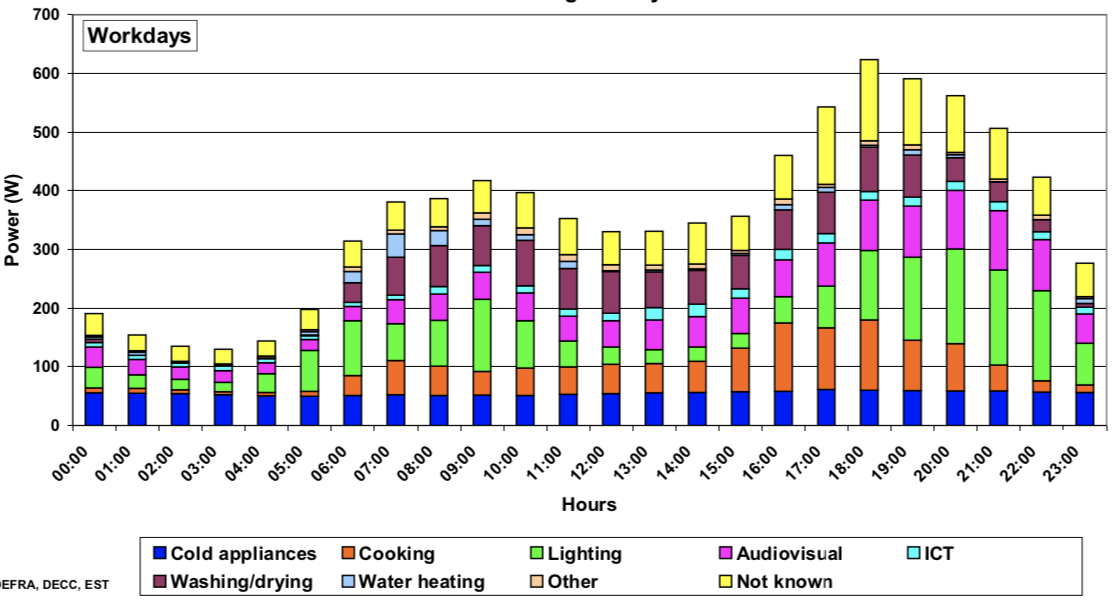
\includegraphics[scale=1.4]{allapp}}
        \caption{Daily average curve of all appliances}
        \label{fig_all_app}
    \end{figure}
    \begin{figure}[ht]
        \centerline{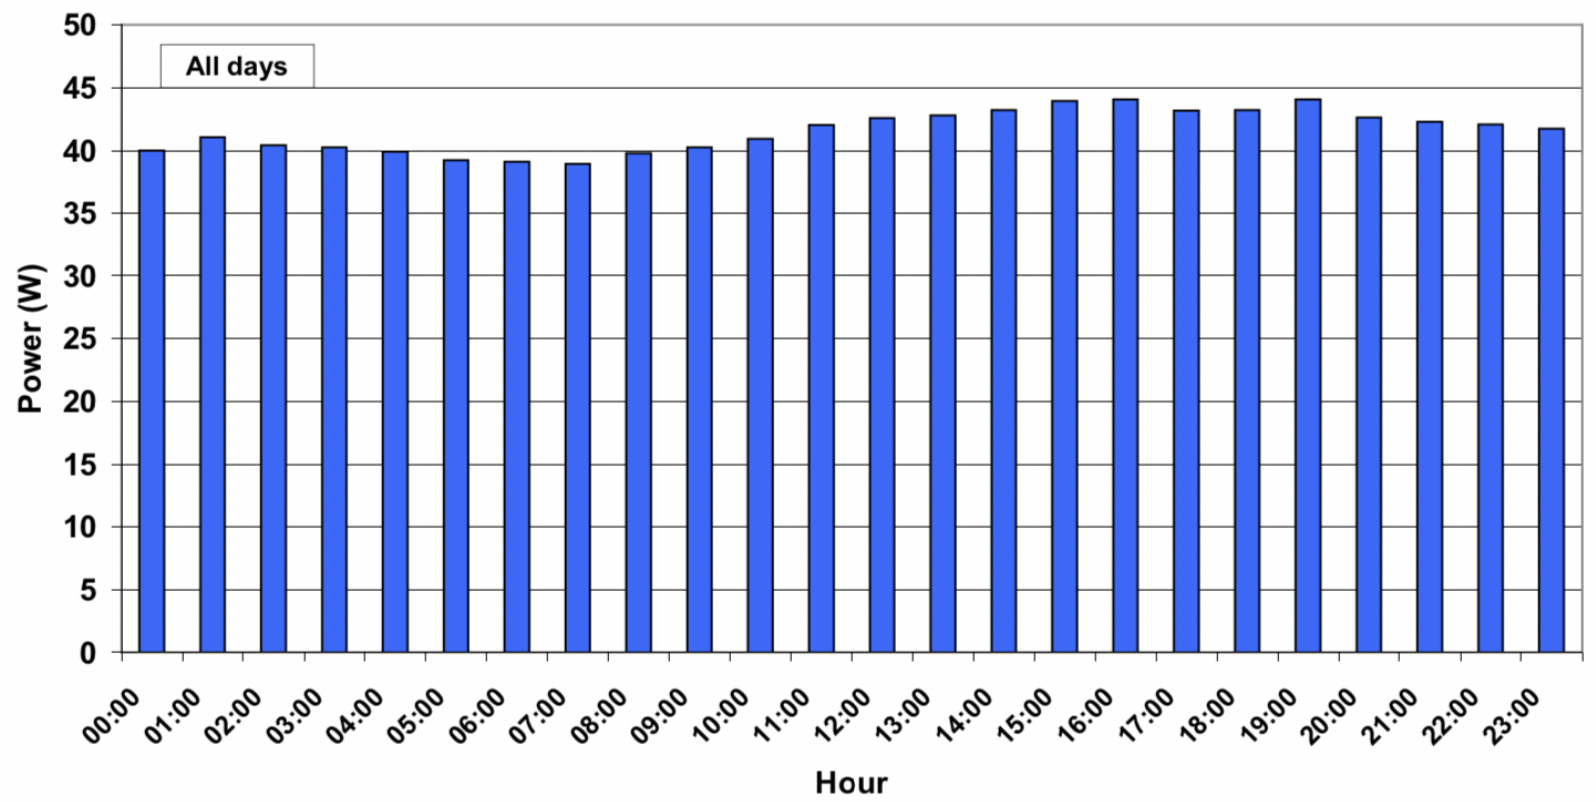
\includegraphics[scale=1]{chestfreezer}}
        \caption{Daily average curve of refrigerator}
        \label{fig_refrigerator}
    \end{figure}
    \begin{figure}[ht]
        \centerline{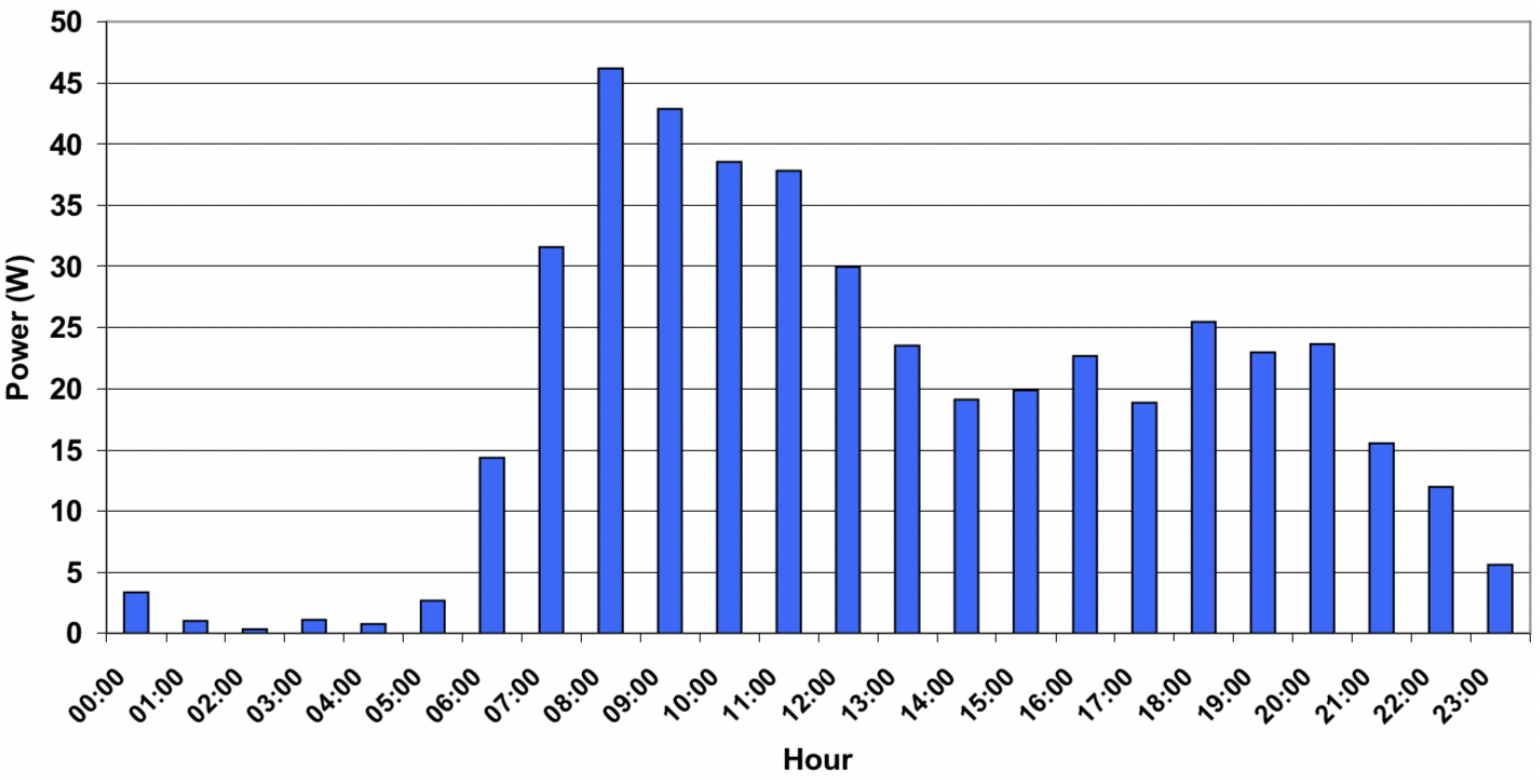
\includegraphics[scale=1]{washingmachine}}
        \caption{Daily average curve of washing machine}
        \label{fig_washing_machine}
    \end{figure}
    \begin{figure}[ht]
        \centerline{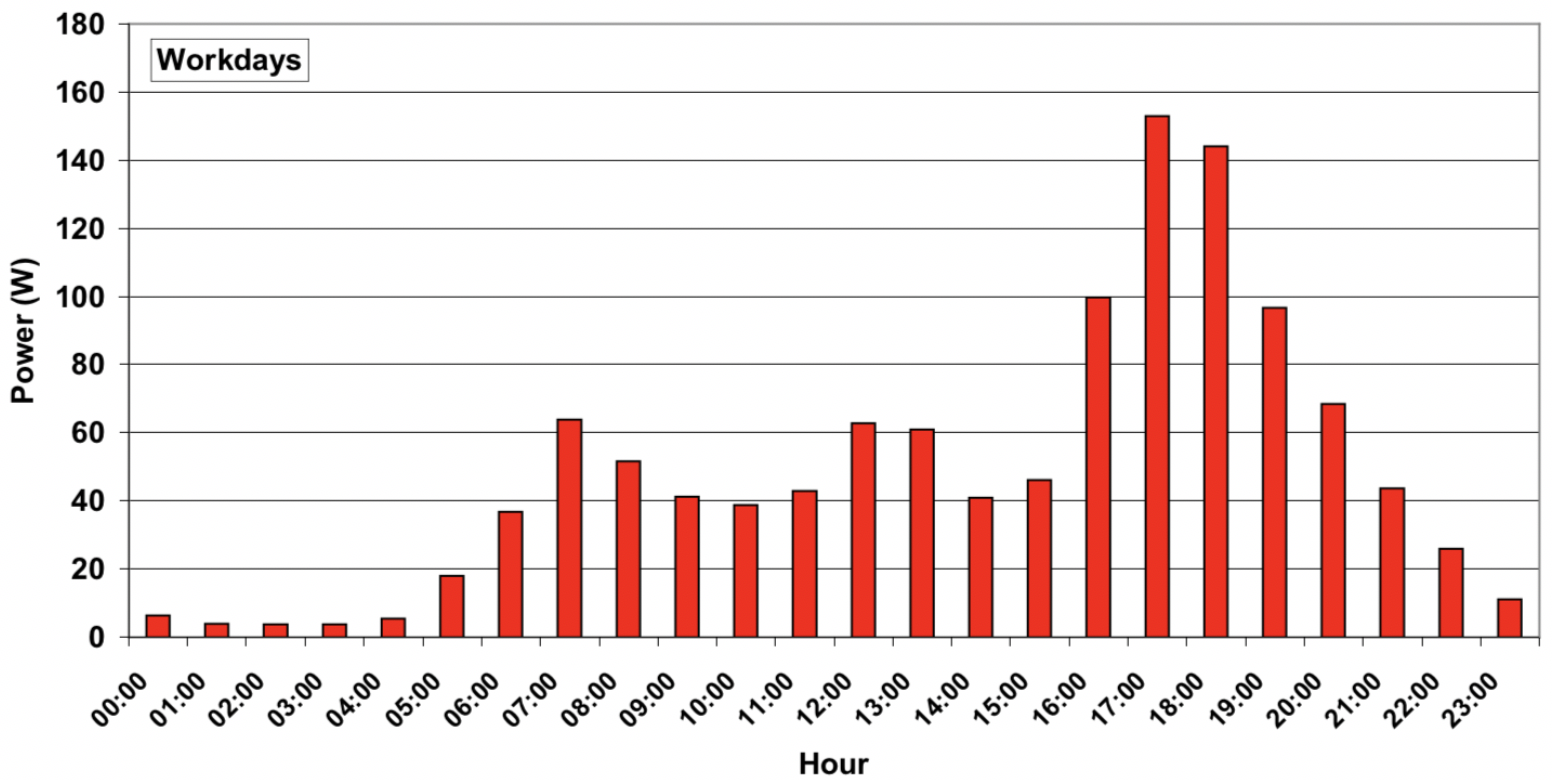
\includegraphics[scale=1]{cooking}}
        \caption{Daily average curve of cooking}
        \label{fig_cooking}
    \end{figure}
    \begin{figure}[ht]
        \centerline{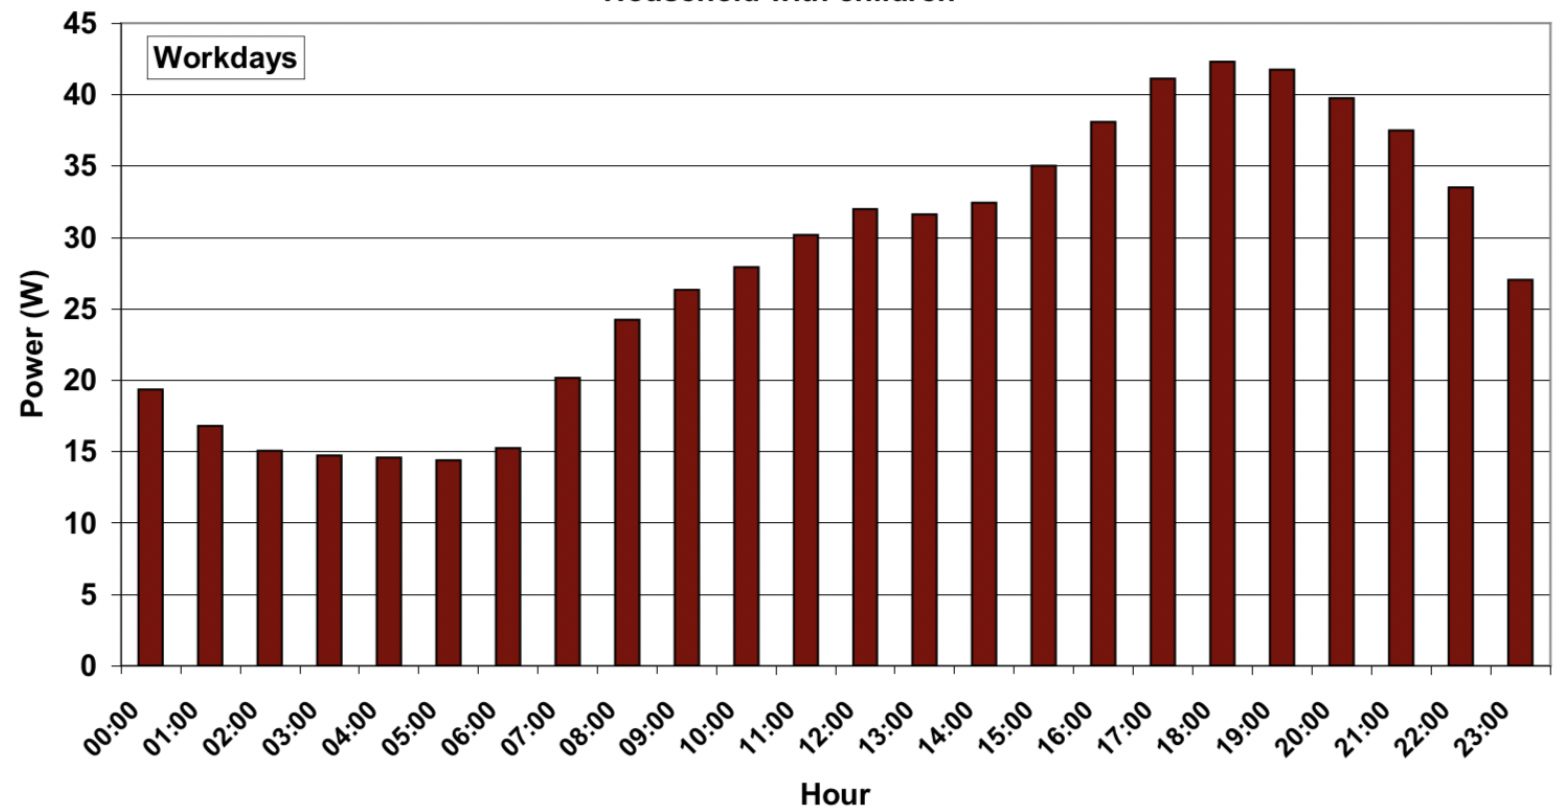
\includegraphics[scale=1]{computer}}
        \caption{Daily average curve of computer}
        \label{fig_computer}
    \end{figure}
    \begin{figure}[ht]
        \centerline{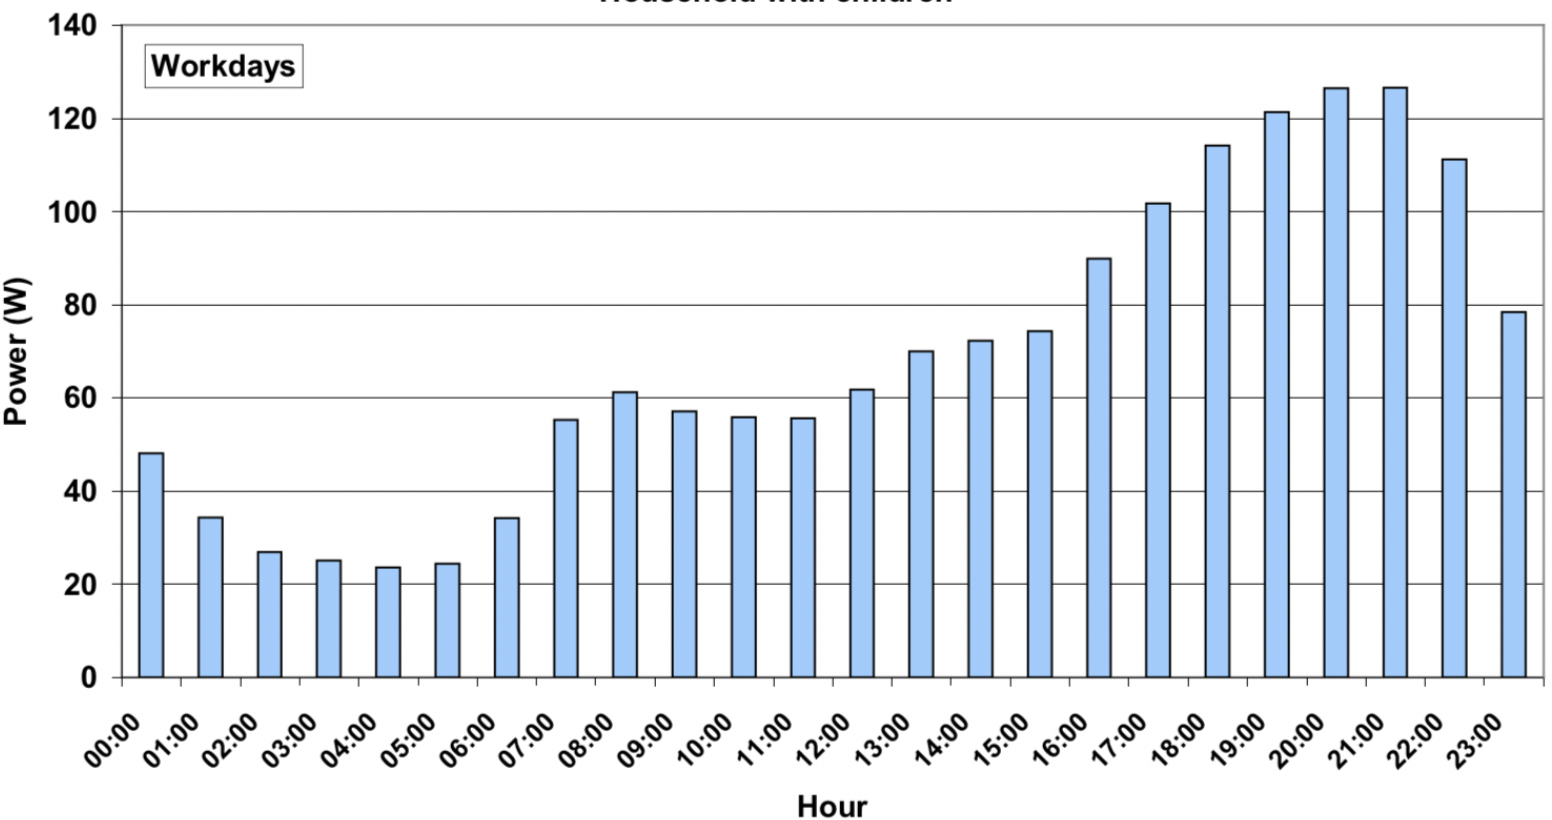
\includegraphics[scale=1]{audiovisual}}
        \caption{Daily average curve of audiovisual}
        \label{fig_audiovisual}
    \end{figure}
    \begin{figure}[ht]
        \centerline{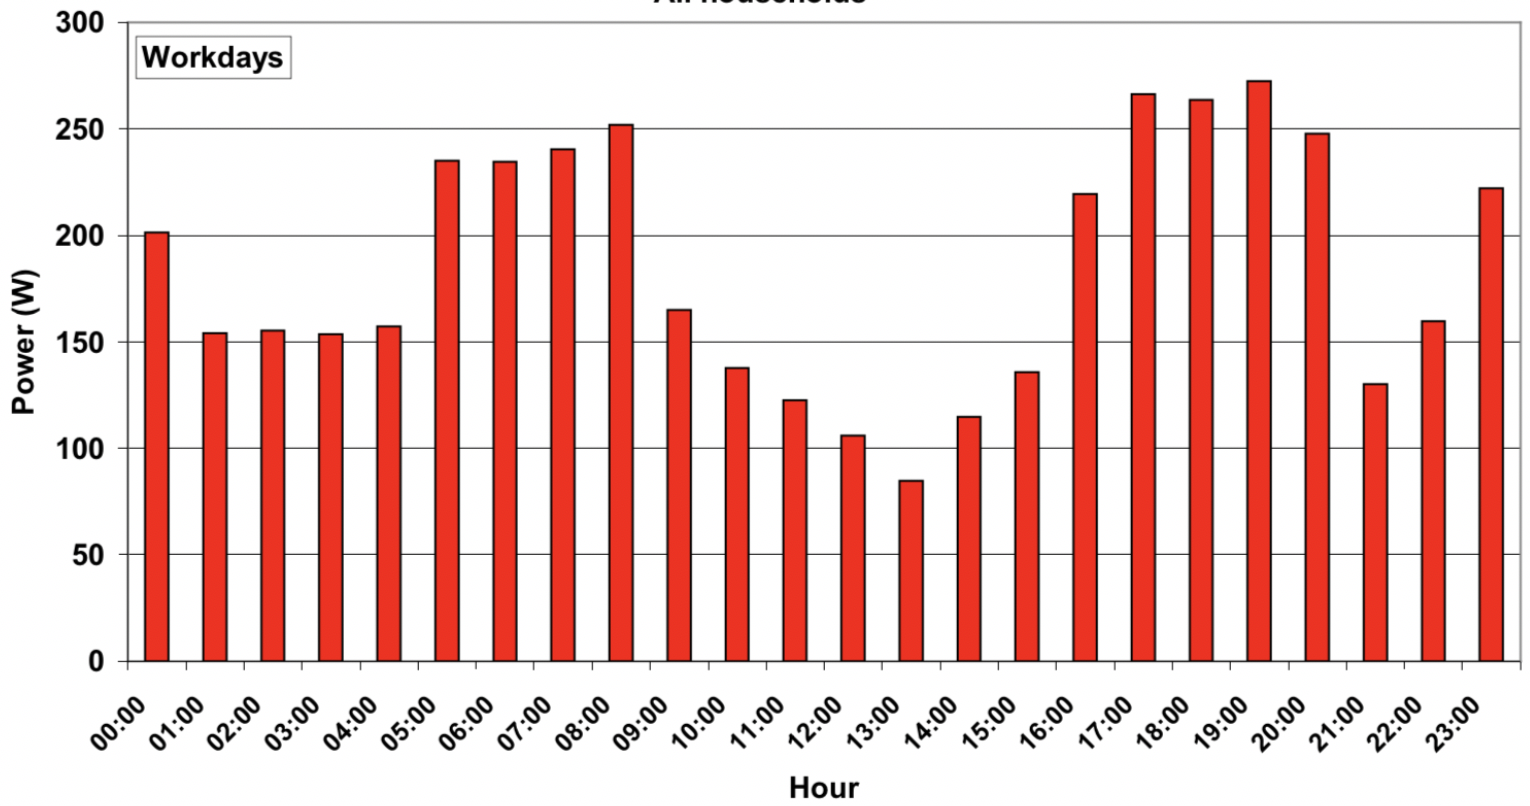
\includegraphics[scale=1]{heating}}
        \caption{Daily average curve of heating}
        \label{fig_heating}
    \end{figure}
    \begin{figure}[ht]
        \centerline{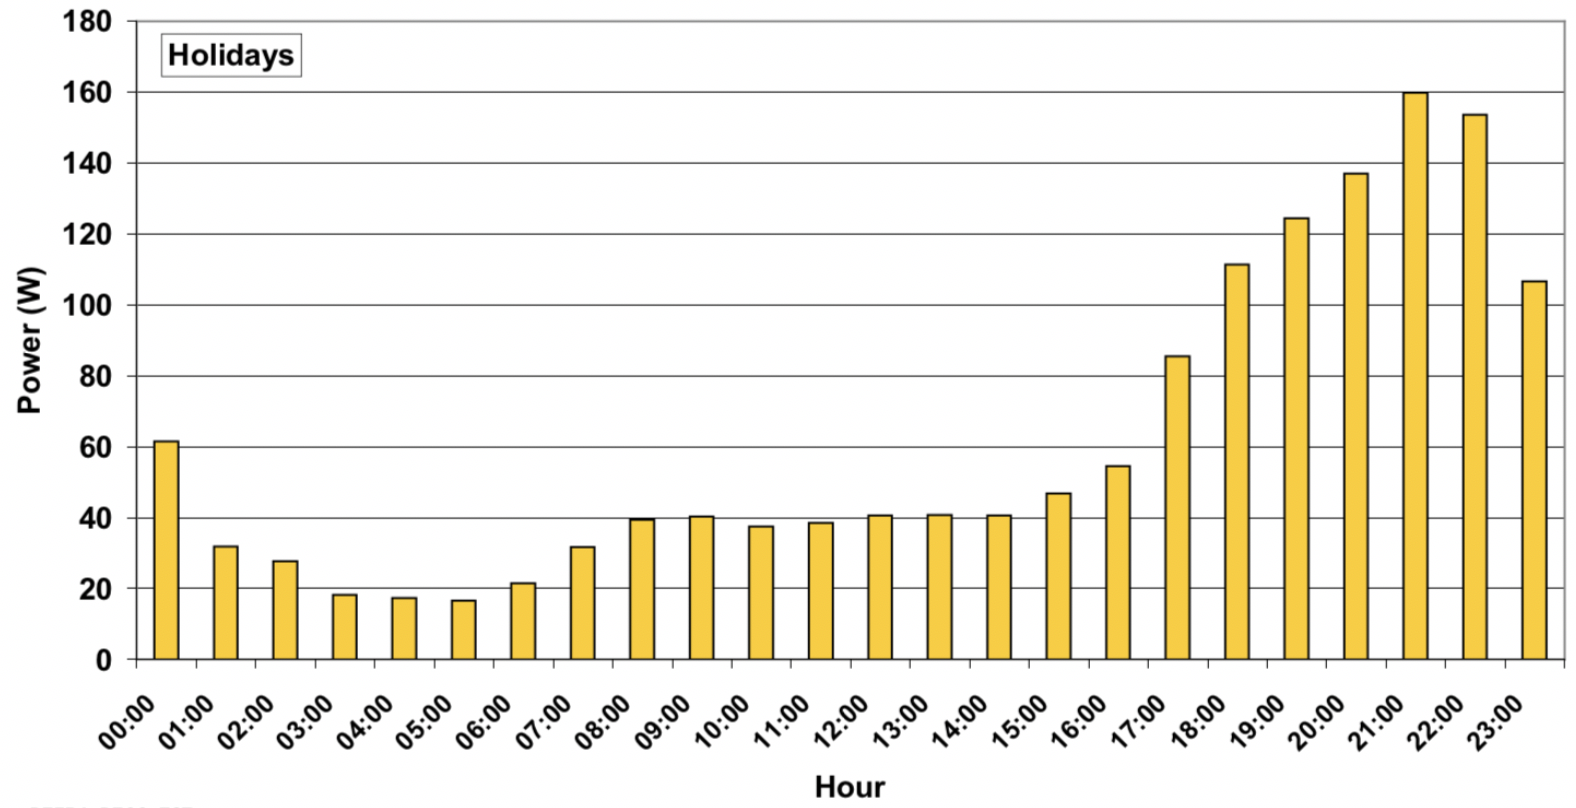
\includegraphics[scale=1]{lighting}}
        \caption{Daily average curve of lighting}
        \label{fig_lighting}
    \end{figure}

    \begin{figure}[ht]
        \centerline{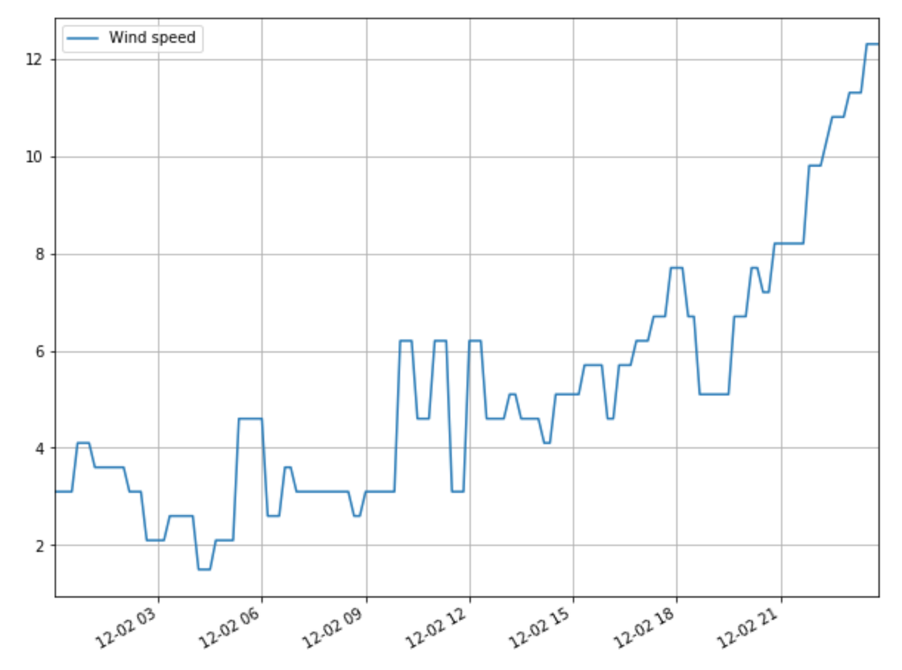
\includegraphics[scale=1]{1202}}
        \caption{The wind speed with a typical increasing tendency}
        \label{fig_1202}
    \end{figure}

    \begin{figure}[ht]
        \centerline{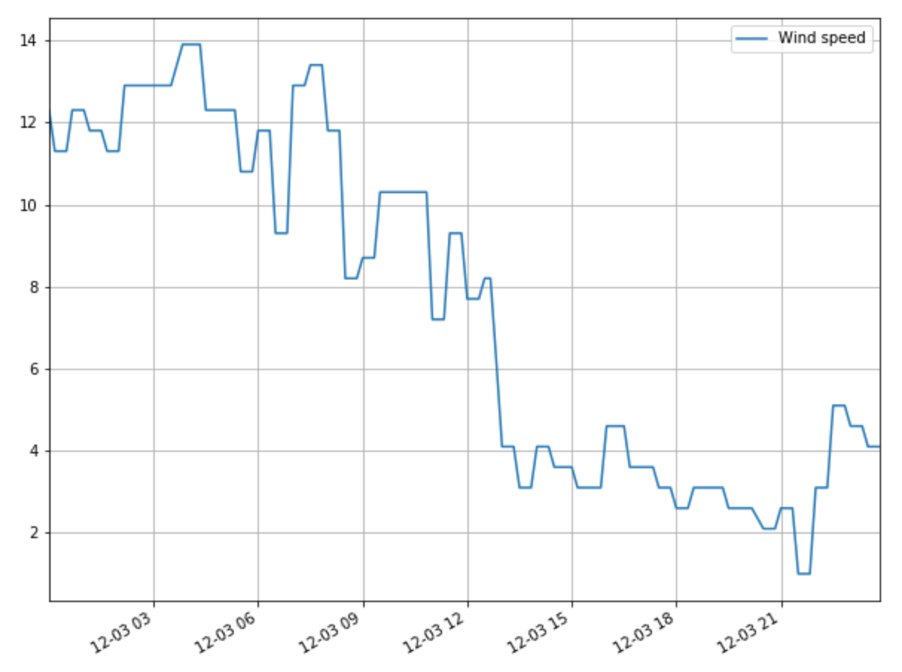
\includegraphics[scale=1]{1203}}
        \caption{The wind speed with a typical decreasing tendency}
        \label{fig_1203}
    \end{figure}

    \begin{figure}[ht]
        \centerline{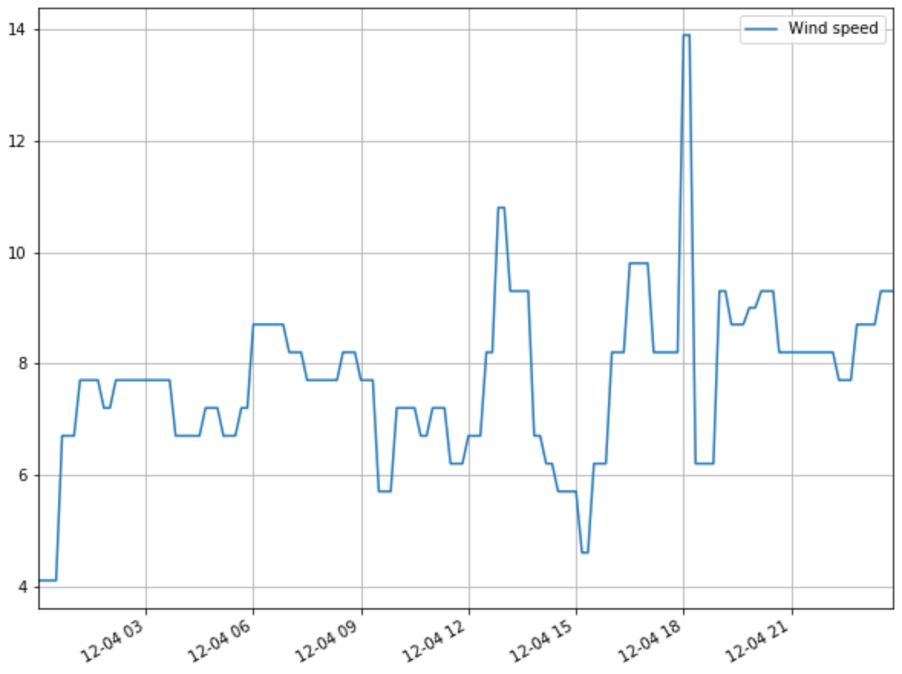
\includegraphics[scale=1]{1204}}
        \caption{The wind speed with a high level}
        \label{fig_1204}
    \end{figure}

    \begin{figure}[ht]
        \centerline{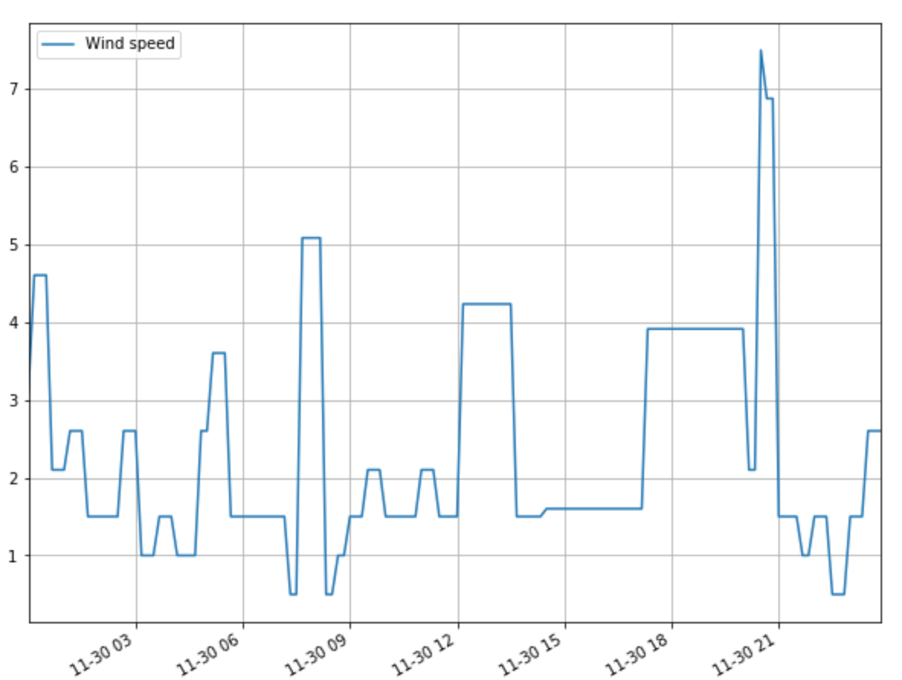
\includegraphics[scale=1]{1130}}
        \caption{The wind speed with a low level}
        \label{fig_1130}
    \end{figure}

    \begin{figure}[ht]
        \centerline{\includegraphics[scale=1]{1107}}
        \caption{The wind speed with a level near the global mean}
        \label{fig_1107}
    \end{figure}

    \begin{figure}[ht]
        \centerline{\includegraphics[scale=1.95]{extreme_case}}
        \caption{An illustration of an extreme case on November 30th. The upper chart is the condition of curtailment, where no curtailment was happened on this day. The bottom chart the subtraction of power generation and demand.}
        \label{fig_extreme_case}
    \end{figure}


    \cleardoublepage  
    \phantomsection  
    \addcontentsline{toc}{chapter}{Bibliography}
    \begin{thebibliography}{99}
        % \bibitem{latexcompanion} 
        % Michel Goossens, Frank Mittelbach, and Alexander Samarin. 
        % \textit{The \LaTeX\ Companion}. 
        % Addison-Wesley, Reading, Massachusetts, 1993.
        
        % \bibitem{knuthwebsite} 
        % Knuth: Computers and Typesetting,
        % \\\texttt{http://www-cs-faculty.stanford.edu/\~{}uno/abcde.html}

        \bibitem{structureandinterpretationofcomputingprograms} 
        Abelson, Harold and Sussman, Gerald Jay. and Sussman, Julie. 
        \textit{Structure and interpretation of computer programs}. 
        MIT Press, London, 1996.

        \bibitem{handsonmachinelearning} 
        Géron, Aurélien and Demarest, Rebecca. 
        \textit{Hands-on machine learning with Scikit-Learn and TensorFlow: concepts, tools, and techniques to build intelligent systems}. 
        OReilly, Sebastopol, 2019.

        \bibitem{goodfellow} 
        Goodfellow, Ian and Bengio, Yoshua and Courville, Aaron. 
        \textit{Deep learning}. 
        The MIT Press, Cambridge, MA, 2017.

        \bibitem{probability} 
        DeGroot, Morris H. and Schervish, Mark J. 
        \textit{Probability and statistics}. 
        Pearson Education, Inc., Hoboken, NJ, 2019.

        \bibitem{c++primer} 
        Lippman, Stanley B. and Lajoie, Josee and Moo, Barbara E. 
        \textit{C++ Primer}. 
        Addison-Wesley, Inc., Boston, 2013.

        \bibitem{gilbert} 
        Strang, Gilbert. 
        \textit{Introduction to linear algebra}. 
        Wellesley - Cambridge Press, Wellesley MA, 2016.



    \end{thebibliography}
    \renewcommand{\bibname}{References}

    \cleardoublepage  
    \phantomsection  
    \addcontentsline{toc}{chapter}{References}
    \bibliographystyle{IEEEtran}
    \bibliography{dissertation}
\end{document}